\documentclass[12pt,a4paper,twoside,openany]{book}
\usepackage{amsmath, amssymb, amsfonts, amsthm, mathtools, bm, derivative}
\usepackage[utf8]{inputenc}
\usepackage[paperheight=10.75in,paperwidth=8.25in,margin=1in,heightrounded]{geometry}
\usepackage[english,greek]{babel}
\author{Θεμιστοκλής Δημητριάδης\\Τμήμα Μαθηματικών ΑΠΘ}
\title{Αρχές χρηματοοικονομικών μαθηματικών και εφαρμογή μοντέλων στην αποτίμηση δικαιωμάτων}
\date{}
\usepackage{enumitem}
\usepackage[T1]{fontenc}
\usepackage{txfonts}
%\usepackage{mathptmx}
%\usepackage{lmodern}
%\usepackage{newtxtext}
%\usepackage{newtxmath} % If you also want the math font to be Times Roman
\usepackage{graphicx}
\usepackage{fancyhdr}
\usepackage{dsfont}
\usepackage{hyperref}
\usepackage{setspace}
\usepackage{amsthm}
\usepackage{physics}
\usepackage{tcolorbox}
%\usepackage{minted}

\newtheorem{theorem}{\textit{Θεώρημα}}[section]
\newtheorem{definition}{\textit{Ορισμός}}[section]
\newtheorem{lemma}[theorem]{\textit{Λήμμα}}
\newtheorem{statement}{\textit{Πρόταση}}[section]

\hypersetup{colorlinks=true, urlcolor= cornellred, linkcolor= black, citecolor= darkmagenta} %linkcolor= carmine
%\pagestyle{fancy}

\newcommand{\probP}{\selectlanguage{english}\text{I\kern-0.15em P}} 

% Για να περάσω python κώδικα
\usepackage{pythonhighlight}

\usepackage{listings}
\usepackage{color}

\definecolor{codegray}{rgb}{0.5,0.5,0.5}
\definecolor{backcolour}{rgb}{0.95,0.95,0.94}

\definecolor{darkmagenta}{rgb}{0.55, 0.0, 0.55}
\definecolor{cornellred}{rgb}{0.7, 0.11, 0.11}
\definecolor{darkbyzantium}{rgb}{0.36, 0.22, 0.33}
\definecolor{carmine}{rgb}{0.59, 0.0, 0.09}
\definecolor{ecru}{rgb}{0.76, 0.7, 0.5}
\definecolor{egyptianblue}{rgb}{0.06, 0.2, 0.65}
\definecolor{lava}{rgb}{0.81, 0.06, 0.13}
\definecolor{patriarch}{rgb}{0.5, 0.0, 0.5}
\definecolor{darkcyan}{rgb}{0.0, 0.55, 0.55}


\lstdefinestyle{mystyle}{
	language=Python,
	backgroundcolor=\color{backcolour},   
	commentstyle=\color{darkcyan},
	keywordstyle=\color{lava},
	numberstyle=\tiny\color{codegray},
	stringstyle=\color{patriarch},
	basicstyle=\footnotesize\ttfamily,,
	breakatwhitespace=false,         
	breaklines=true,                 
	captionpos=b,                    
	keepspaces=true,                 
	numbers=left,                    
	numbersep=5pt,                  
	showspaces=false,                
	showstringspaces=false,
	showtabs=false,                  
	tabsize=4
}
\lstset{style=mystyle}   
                      
%--------------------------------------------------------------------------
% 		HEADER & FOOTER 
%--------------------------------------------------------------------------
\RequirePackage{tikz}
\RequirePackage{tkz-tab}
\usetikzlibrary{positioning}
\usetikzlibrary{shapes.geometric, arrows}
% ----- Header and footer -----
\RequirePackage{fancyhdr}
\pagestyle{fancy}
\fancyhead[RO,LE]{%
	\tikz[baseline=(char.base)]{
		\node[shape=rectangle,fill=black,text=white,inner sep=2pt] (char) {\thepage};
	}
} % Page number in a small black box

\fancyhead[RE,LO]{\nouppercase{\leftmark}} % chapter name and number on the right for even pages and left for odd pages in the header
\renewcommand{\headrulewidth}{3pt} % sets thickness of header line
\renewcommand{\chaptermark}[1]{\markboth{#1}{}}
\fancyfoot{} % removes page number on bottom of page

% ----- Header of the frontpage ----- 
\fancypagestyle{frontpage}{
	\fancyhf{}
	\renewcommand{\headrulewidth}{0pt}
	\renewcommand{\footrulewidth}{0pt}
	\vspace*{1\baselineskip}
	
	\fancyhead[R]{École Nationale de Commerce et de Gestion
		\linebreak       Casablanca, 2020\vspace*{.5\baselineskip}}
	% change to nhhlogo1.png for golden NHH logo
}

% %--------------------------------------------------------------------------
% % 		Chapters and sections 
% %--------------------------------------------------------------------------
\renewcommand\thesubsubsection{\arabic{subsection}.\roman{subsubsection}}
\renewcommand\thesubsection{\thesection.\arabic{subsection}}
\renewcommand\thesection{\arabic{section}}

\makeatletter
\@addtoreset{chapter}{part} % for numberring
\makeatother  

\RequirePackage[titles]{tocloft}

\RequirePackage{titletoc}
% Define a new command to create per-chapter mini-TOCs
\newcommand{\chaptertoc}{%
	\startcontents[chapters]
	\printcontents[chapters]{}{1}{\setcounter{tocdepth}{1}}
	\vspace{0.5cm}
}

\newcommand{\intro}[1]{
	\noindent
	\begin{minipage}[t]{0.48\textwidth}
		\chaptertoc
	\end{minipage}%
	\hfill
	\begin{minipage}[t]{0.48\textwidth}
		#1
	\end{minipage}
	\newpage
}


\RequirePackage[explicit]{titlesec}
\RequirePackage{titlesec}

\titleformat{\chapter}[display]
{\centering\normalfont\Huge}
{\titlerule[5pt]\vspace{3pt}\titlerule[2pt]\vspace{3pt}\textbf{\MakeUppercase{\chaptername} \thechapter}}
{0pt}
{\titlerule[2pt]\vspace{1pc}\Huge\MakeUppercase{#1}}

\titleformat{name=\chapter,numberless}[display]
{  \centering\normalfont\Huge}
{\titlerule[2pt]\vspace{-20pt}}
{0pt}
{\Huge\MakeUppercase{#1} \addcontentsline{toc}{chapter}{#1} }


% %--------------------------------------------------------------------------
% %         Begin Document
% %--------------------------------------------------------------------------
\begin{document}
\setstretch{1.2}
% Customize title page appearance
\begin{titlepage}
	\centering
	% Custom color and font settings
	\vspace*{2cm}  % Adjust vertical spacing
	{\Huge\textbf{\textcolor{black}{Εισαγωγή στα Χρηματοοικονομικά Μαθηματικά. Εφαρμογή με μοντελοποίηση στην αποτίμηση δικαιωμάτων με χρήση του στοχαστικού μοντέλου \selectlanguage{english}Heston\selectlanguage{greek}}}} \\[1cm]
	{\Huge\textit{ΕΙΔΙΚΟ ΘΕΜΑ}} \\[0.5cm]
	\rule{16cm}{1mm} \\[0.4cm]  % Decorative line
	{\LARGE Θεμιστοκλής Δημητριάδης \\ Τμήμα Μαθηματικών Α.Π.Θ} \\[1.5cm]
	
	% Decorative box (Optional)
	\begin{tcolorbox}[colback=gray!20, colframe=gray!80, width=0.6\textwidth, center title, title=\selectlanguage{english}Keywords]
		Κίνηση \selectlanguage{english}Brown\selectlanguage{greek}, Χρόνος Πρώτης Άφιξης, Αρχή Αντανάκλασης, Γεωμετρική Κίνηση \selectlanguage{english}Brown\selectlanguage{greek}, Στοχαστικός Λογισμός, Λημμα \selectlanguage{english}Itô\selectlanguage{greek}, Δικαιώματα Προαίρεσης Απλά και \selectlanguage{english}Barrier\selectlanguage{greek}, Μοντέλο \selectlanguage{english}Black-Scholes\selectlanguage{greek}, Μέθοδος \selectlanguage{english}LSM\selectlanguage{greek}, Μοντέλο \selectlanguage{english}Heston\selectlanguage{greek}, \selectlanguage{english}Trust Region Reflective\selectlanguage{greek}, \selectlanguage{english}Simulated Annealing\selectlanguage{greek}, Προσομοιώσεις \selectlanguage{english}Monte-Carlo\selectlanguage{greek}, \selectlanguage{english}S\&P 500\selectlanguage{greek}
	\end{tcolorbox}
	
	\vfill
	% Footer text (optional)
	{\Large \textit{Επιβλέπων: Γεώργιος Τσακλίδης\\Καθηγητής Α.Π.Θ}} \\[1cm]
	% Date (Optional)
	{\large \textit{Ημερομηνία: Οκτώβριος 2024}} %\\[0.5cm]
\end{titlepage}

\tableofcontents % Prints the main table of contents

%\listoffigures % Prints the list of figures

\chapter{Κίνηση \selectlanguage{english}Brown}	
		Ο βοτανολόγος \selectlanguage{english}Robert Brown \selectlanguage{greek}το 1827, μελετώντας γυρεόκοκκους που αιωρούνταν στο νερό, παρατήρησε μικροσκοπικά σωματίδια, που εκτοξεύονταν από αυτούς, να κινούνται με έναν ακανόνιστο τυχαίο τρόπο. Το 1900 ο μαθηματικός \selectlanguage{english}Louis Bachelier \selectlanguage{greek}στην διδακτορική του διάτριβη \selectlanguage{english}"The theory of speculation"\selectlanguage{greek} χρησιμοποίησε την κίνηση \selectlanguage{english}Brown \selectlanguage{greek}για να περιγράψει τις διακυμάνσεις της αγοράς που επηρεάζουν την τιμή ενος περιουσιακού στοιχείου. Ο \selectlanguage{english}Albert Einstein \selectlanguage{greek}το 1905 θεώρησε την κίνηση \selectlanguage{english}Brown \selectlanguage{greek}ως ενα στοχαστικό μοντέλο για την περιγραφή της κίνησης ενος σωματιδίου μέσα σε υγρό που οφείλεται στην σύγκρουσή του με τα μόρια του υγρού. Ο αυστηρός μαθηματικός ορισμός της, είναι επίτευγμα του \selectlanguage{english}Norbert Wiener \selectlanguage{greek}το 1923, και για αυτό σε πολλά συγγράμματα ονομάζεται και διαδικασία \selectlanguage{english}Wiener\selectlanguage{greek}. Σήμερα η κίνηση \selectlanguage{english}Brown \selectlanguage{greek} βρίσκει εφαρμογές και σε πολλές άλλες επιστήμες όπως τα οικονομικά, την βιολογία και την σεισμολογία.
	\vspace{2.5mm}\\
		Σε αυτό το κεφάλαιο θα ασχοληθούμε με την κατασκευή της κίνησης \selectlanguage{english}Brown, \selectlanguage{greek} θα δώσουμε τον ορισμό της και θα αναφερθούμε στις πιο σημαντικές της ιδιότητες.
		%Μια στοχαστική διαδικασία, όπως είναι η κίνηση \selectlanguage{english}Brown\selectlanguage{greek}, περιγράφει ένα φαινόμενο που εξελίσσεται στον χρόνο, παρουσιάζοντας ένα βαθμό τυχαιότητας. Μπορεί επομένως να θεωρηθεί ως μια συνάρτηση του χρόνου και ενός τυχαίου παράγοντα. 
	\section{Ορισμοί}
	\vspace{2.5mm}
		Πριν ξεκινήσουμε θα ορίσουμε μερικές βασικές έννοιες από την θεωρία Μέτρου και την θεωρία Πιθανοτήτων, σχετικές με αυτά που ακολουθούν.
		
		\begin{definition}[$\sigma$-άλγεβρα]
			Μια $\sigma$-άλγεβρα $\mathcal{F}$ στον $\Omega$ είναι μια συλλογή υποσυνόλων του $\Omega$ για την οποία ισχύουν
			\begin{itemize}
				\item $\emptyset,\Omega\in\mathcal{F}$
				\item Αν $A\in\mathcal{F}$ τότε $A^\mathsf{c}\in\mathcal{F}$
				\item Αν $\{A_i\}_{i\in I}$ είναι μια οικογένεια συνόλων της $\mathcal{F}$, τότε η αριθμήσιμη ένωση\\ $\bigcup\limits_{i\in I}^{} A_i \in\mathcal{F}$
			\end{itemize}
		\end{definition}
		
		\begin{definition}[Φιλτράρισμα]
			Έστω $\Omega$ ένας πεπερασμένος δειγματοχώρος. Ονομάζουμε φιλτράρισμα, μια ακολουθία από $\sigma$-άλγεβρες του $\Omega$, $\mathcal{F}_0, \mathcal{F}_1, \mathcal{F}_2,\dots, \mathcal{F}_n$ τέτοιες ώστε \\$\mathcal{F}_0\subset \mathcal{F}_1\subset \mathcal{F}_2\subset\dots\subset \mathcal{F}_n$.
		\end{definition}
	
		\begin{definition}[Χώρος Πιθανοτήτων]
			Η τριπλέτα $(\Omega,\mathcal{F},\probP)$ καλείται χώρος πιθανοτήτων αν το $\Omega$ είναι μη κενό σύνολο που περιέχει ολα τα δυνατά αποτελέσμάτα ενός πειράματος τύχης (Δειγματοχώρος), $\mathcal{F}$ είναι μια $\sigma$-άλγεβρα υποσυνόλων του $\Omega$ και $\probP$ είναι ένα μέτρο πιθανότητας ορισμένο πάνω στην $\mathcal{F}$.
		\end{definition}
		\begin{definition}[Στοχαστική Διαδικασία]
			Μια στοχαστική διαδικασία είναι μια ακολουθία τυχαίων μεταβλητών $\{X_t\}_{t\geq0}$, ορισμένων σε έναν χώρο πιθανοτήτων, που αντιπροσωπεύουν την εξέλιξη κάποιου συστήματος με τυχαίες τιμές κατα τη πάροδο του χρόνου.
		\end{definition}
		\begin{definition}[\selectlanguage{english}Borel\selectlanguage{greek} $\sigma$-άλγεβρα]
			Συμβολίζουμε ως $\mathcal{B}(\mathbb{R})$ την μικρότερη $\sigma$-άλγεβρα η οποία περιέχει όλα τα ανοιχτά διαστήματα του $\mathbb{R}$.
		\end{definition}
		\begin{definition}[$\mathcal{F}$-μετρήσιμη]
			Έστω $(\Omega,\mathcal{F},\probP)$ χώρος πιθανοτήτων και έστω απεικόνιση $X:\Omega\rightarrow\mathbb{R}$ ορισμένη στο $\Omega$. Η αντίστροφη απεικόνιση της $X$ είναι\\ \centerline{$X^{-1}(A)= \{\omega\in\Omega: X(\omega)\in A\}$, όπου $A\in\mathcal{B}(\mathbb{R})$.} Aν $X^{-1}(A)\in\mathcal{F}$για κάθε $A\in\mathcal{B}(\mathbb{R})$ τότε λέμε ότι η $X$ είναι $\mathcal{F}$-μετρήσιμη.
		\end{definition}
		
			\noindent Παρατηρούμε ότι η αντίστροφη συνάρτηση της $X$ στον παραπάνω ορισμό είναι ακριβώς το ενδεχόμενο $\{X\in A\}$. Θέλουμε να μετρήσουμε την πιθανότητα του $X$ να ανήκει σε ένα υποσύνολο του $\mathbb{R}$, δηλαδή την $\probP[\{X\in A\}]$. Για να γίνει όμως αυτό πρέπει $\{X\in A\}\in\mathcal{F}$ για κάθε $A\in\mathcal{B}(\mathbb{R})$ αφου το μέτρο πιθανότητας $\probP$ ορίζεται μόνο στην $\sigma$-άλγεβρα $\mathcal{F}$.\\ Ο ορισμός της τυχαίας μεταβλητής είναι ισοδύναμος με τον ορισμό της $\mathcal{F}$-μετρήσιμης απεικόνισης.
		
		\begin{definition}
			Θα λέμε ότι μια ακολουθία τυχαίων μεταβλητών $\{X_t\}_{t\geq0}$ είναι προσαρμοσμένη στο φιλτράρισμα $\{\mathcal{F}_t\}_{t\geq0}$ αν για κάθε $t$ ισχύει ότι η $X_t$ είναι $\mathcal{F}_t$-μετρήσιμη
		\end{definition}
	
		\begin{definition}[\selectlanguage{english}Martingale]
			Έστω $(\Omega,\mathcal{F},\probP)$ χώρος πιθανοτήτων και έστω μια στοχαστική διαδικασία $\{X(t)\}_{t\in T}$ σε χρόνο συνεχή όπου $T$ ένα οποιοδήποτε διάστημα της ευθείας των πραγματικών αριθμών. Για κάθε $s,t\in T$ με $s<t$ υποθέτουμε ότι $\mathcal{F}(s)$ και $\mathcal{F}(t)$ είναι $\sigma$-άλγεβρες στον $\Omega$ τέτοιες ώστε $\mathcal{F}(s)\subset\mathcal{F}(t)$\\
			Η  $\{X(t)\}_{t\in T}$ θα είναι ένα \selectlanguage{english}Martingale\selectlanguage{greek} σε σχέση με την οικογένεια των $\sigma$-αλγεβρών $\{\mathcal{F}(t)\}_{t\in T}$ αν για όλα τα $t\in T$ ισχύουν οι συνθήκες
			\begin{itemize}
				\item Η $\{X(t)\}_{t\in T}$ είναι προσαρμοσμένη στο φιλτράρισμα $\{\mathcal{F}(t)\}_{t\in T}$.
				\item $\mathbb{E}[|X(t)|]<\infty$ για κάθε $t\in T$.
				\item $\mathbb{E}[X(t)\mid\mathcal{F}(s)]= X(s)$ για κάθε $0\leq s<t\leq T$.
			\end{itemize}
		Ο ορισμός σε διακριτό χρόνο είναι παρόμοιος.
		\end{definition}
	
	
	\section{Συμμετρικός τυχαίος περίπατος}
	\vspace{2.5mm}
		Για την κατασκευή της κίνησης \selectlanguage{english}Brown\selectlanguage{greek} ξεκινάμε με έναν συμμετρικό τυχαίο περίπατο. Ας θεωρήσουμε ένα σωματίδιο που κινείται ανα μονάδα χρόνου όπως δηλώνει η τυχαία μεταβλητή 
		\[ 
		X_i = 
		\begin{cases} 
			+1 \text{, με πιθανότητα 1/2}\\
			-1 \text{, με πιθανότητα 1/2}
		\end{cases}
		\]\\
		Ορίζουμε για λόγους ευκολίας $M_0=0$, δηλαδή το σωματίδιο ξεκίνα την πορεία του απο την αρχή των αξόνων. Η τυχαία μεταβλητή που δηλώνει την θέση του σωματιδίου την χρονική στιγμή \selectlanguage{english}k\selectlanguage{greek} είναι 
		\[M_k= \sum_{i=1}^{k} X_i, \quad k =1,2,... \]\\
		Η στοχαστική διαδικασία $M_k, k=0,1,2,...$ καλείται συμμετρικός τυχαίος περίπατος και είναι μια στοχαστική διαδικασία σε διακριτό χρόνο και χώρο καταστάσεων.\\Ονομάζεται συμμετρικός επειδή $\probP[X_i=1]=\probP[X_i=-1]$.\\
		
		\begin{figure}[h]
			\centering
			\includegraphics[width=1\textwidth]{Figure_RW.png}
			\caption{Οκτώ βήματα ενος τυχαίου περιπάτου.}
			\label{fig:SymmRndWalk}
			\vspace{4mm}
		\end{figure}
		
		\noindent Αν υποθέσουµε τώρα ότι το σωµατίδιο έχει ως αρχική θέση  $X_0 = 0$,  τότε η θέση του  $Xn$  µετά από  άρτιο αριθµό βηµάτων  $n = 2k$  $(k = 1, 2, ...)$  θα είναι άρτια και συγκεκριµένα θα είναι µια από τις $\{-2k, -2k-2,..., 0, ..., 2k-2, 2k\}$,  ενώ µετά από περιττό αριθµό βηµάτων  $n = 2k+1$  θα είναι περιττή και συγκεκριµένα θα είναι µια από τις  $\{-2k-1, -2k-3,...,-1, 1, ..., 2k-1, 2k+1\}$.
		\vspace{2.5mm}\\
		Η πιθανότητα με την οποία βρίσκεται το σωματίδιο σε μία από τις παραπάνω θέσεις υπολογίζεται με τον εξής τρόπο. Θεωρούμε τις τυχαίες μεταβλητές
		\[Y_i=\frac{1}{2}(X_i+1)\]
		και επομένως
		\[ 
		Y_i = 
		\begin{cases} 
			1 \text{, με πιθανότητα 1/2}\\
			0 \text{, με πιθανότητα 1/2}
		\end{cases}
		\]\\
		Δηλαδή, $Y_i\sim\operatorname{Bernoulli} (\frac{1}{2})$ και ως εκ τούτου το άθροισμα τους $S_n=\sum_{i=1}^{n} Y_i \sim \operatorname {Binomial}(n,\frac{1}{2})$.\\ Τέλος, επειδή $S_n= \frac{1}{2}(M_n+n)$ έχουμε ότι 
		\[\probP[M_n=m] = \probP[S_n=\frac{1}{2}(m+n)] = \binom{n}{\frac{1}{2}(m+n)} p^{\frac{1}{2}(m+n)} (1 - p)^{\frac{1}{2}(n-m)}\]\\όπου επειδή $p=\frac{1}{2}$ καταλήγουμε στην σχέση \[\probP[M_n=m] = \binom{n}{\frac{1}{2}(m+n)} \left(\frac{1}{2}\right)^{n} \]\\
	\vspace{2.5mm}
		Μερικές βασικές ιδιότητες του συμμετρικού τυχαίου περιπάτου είναι:
		\begin{itemize}
			\item $\mathbb{E}[M_k] = \sum_{i=1}^{k}\mathbb{E}[X_i] = 0$, λόγω γραμμικότητας μέσης τιμής.
			\item $\operatorname{Var}(M_k) = \sum_{i=1}^{k}\operatorname{Var}(X_i) = \sum_{i=1}^{k}\mathbb{E}[(X_i-\mathbb{E}[X_i]) ^ 2] = \sum_{i=1}^{k}\mathbb{E}[X_i^2] = k $, αφού οι $X_i$ είναι ανεξάρτητες και ισόνομες τυχαίες μεταβλητές.
			\item Έχει ανεξάρτητες προσαυξήσεις, δηλαδή για μη αρνητικούς ακεραίους τέτοιους ώστε $0=t_0<t_1<...<t_n$, τότε οι τυχαίες μεταβλητές \[M_{t_1}=M_{t_1}-M_{t_0}, M_{t_2}-M_{t_1},..., M_{t_n}-M_{t_{n-1}} \] είναι ανεξάρτητες και ισχύει \[\mathbb{E}[M_{t_{j+1}} - M_{t_{j}}] =  \sum_{i=t_j + 1}^{t_{j+1}}\mathbb{E}[X_i]=0\] 
			\[\operatorname{Var}(M_{t_{j+1}} - M_{t_{j}}) = \operatorname{Var}\left(\sum_{i=t_j + 1}^{t_{j+1}}X_i\right)= 
			\sum_{i=t_j + 1}^{t_{j+1}}\operatorname{Var}(X_i) + \sum_{i,l=t_j+1:i\neq l}^{t_{j+1}} \operatorname{Cov}(X_i,X_l) = 
			\sum_{i=t_j + 1}^{t_{j+1}}1 = t_{j+1}-t_j\]
			
			\item Είναι \selectlanguage{english}Martingale\selectlanguage{greek}, πράγματι για μη αρνητικούς ακεραίους $k<l$ ισχύει
			\begin{align*}
				\mathbb{E}[M_l|\mathcal{F}_k] &= \mathbb{E}[(M_l-M_k)+M_k|\mathcal{F}_k] \\
				&= \mathbb{E}[M_l-M_k|\mathcal{F}_k] + \mathbb{E}[M_k|\mathcal{F}_k] \\
				&= \mathbb{E}[M_l-M_k|\mathcal{F}_k] + M_k \\
				&= \mathbb{E}[M_l-M_k] + M_k \\
				&= M_k
			\end{align*}
			Η δεύτερη ισότητα ισχύει λόγω της γραμμικότητας της δεσμευμένης μέσης τιμής, η τρίτη επειδή η $M_k$ εξαρτάται μόνο από τα πρώτα $k$ βήματα και η τέταρτη λόγω της ανεξαρτησίας των $X_i$.
		\end{itemize}
		
		
	\section{Βαθμωτός τυχαίος περίπατος}
	\vspace{2.5mm}
		Για να προσεγγίσουμε την κίνηση \selectlanguage{english}Brown\selectlanguage{greek} διαλέγουμε $n$ μη αρνητικό ακέραιο και προσαρμόζουμε το βήμα και το χρονικό διάστημα του συμμετρικού τυχαίου περιπάτου
		\[W^{(n)}(t) = \frac{1}{\sqrt{n}}M_{nt}\]
		δεδομένου ότι $nt\in \mathbb{Z}$. Αν $nt\notin \mathbb{Z}$ τότε ορίζουμε $W^{(n)}(t)$ με την μέθοδο της γραμμικής παρεμβολής μεταξύ των τιμών των πιο κοντινών σημείων $s$ και $u$ δεξιά και αριστερά του $t$ για τα οποία ισχύει ότι $ns$ και $nu$ είναι ακέραιοι.
	\vspace{2.5mm}
		\begin{figure}[h]
			\centering
			\includegraphics[width=1\textwidth]{Figure_ScaledRW.png}
			\caption{Ένα μονοπάτι του $W^{(100)}$.}
			\label{fig:ScaledRndWalk}
			\vspace{4mm}
		\end{figure}
	
		\noindent Η διαδικασία $W^{(n)}(t)$ έχει χρονικό βήμα $1/\sqrt{n}$ και είναι γραμμική μεταξύ των χρονικών βημάτων.\\
		Ο βαθμωτός τυχαίος περίπατος διατηρεί τις ιδιότητες του τυχαίου περιπάτου,
		\begin{itemize}
			\item $\mathbb{E}[W^{(n)}(t)] = \frac{1}{\sqrt{n}}\mathbb{E}[M_{nt}] = 0$
			\item $\operatorname{Var}(W^{(n)}(t)) = \frac{1}{n}\operatorname{Var}(M_{nt}) = t$
			\item Αν $0=t_0<t_1<...<t_n$ τέτοια ώστε κάθε $nt_j\in \mathbb{Z}$, τότε οι προσαυξήσεις \[W^{(n)}(t_1)-W^{(n)}(t_0), W^{(n)}(t_2)-W^{(n)}(t_1),...,W^{(n)}(t_n)-W^{(n)}(t_{n-1})\] είναι ανεξάρτητες και ισχύει
		\end{itemize}
		\begin{singlespace}
			\[
				\mathbb{E}[W^{(n)}(t_{j+1})-W^{(n)}(t_j)] = \mathbb{E}\left[\frac{1}{\sqrt{n}}M_{nt_{j+1}}-\frac{1}{\sqrt{n}}M_{nt_j}\right] 
				= \frac{1}{\sqrt{n}}\sum_{i=nt_j + 1}^{nt_{j+1}}\mathbb{E}[X_i]
				= 0
			\]
		 	\begin{align*}
		 		\operatorname{Var}(W^{(n)}(t_{j+1})-W^{(n)}(t_j)) &= \operatorname{Var}\left(\frac{1}{\sqrt{n}}\sum_{i=nt_j + 1}^{nt_{j+1}}X_i\right) 
		 		= \frac{1}{n}\operatorname{Var}\left(\sum_{i=nt_j + 1}^{nt_{j+1}}X_i\right) 
		 		= \frac{1}{n}\sum_{i=nt_j + 1}^{nt_{j+1}}\operatorname{Var}(X_i) \\
		 		&= \frac{1}{n}(nt_{j+1}-nt_j) 
		 		= t_{j+1}-t_j
		 	\end{align*}
	 	\end{singlespace}
	 	\begin{itemize}
			\item Με παρόμοια απόδειξη, συμπεραίνουμε ότι είναι \selectlanguage{english}Martingale\selectlanguage{greek} δηλαδή για μη αρνητικούς ακεραίους $k<l$ ισχύει \[\mathbb{E}[W^{(n)}(l)|\mathcal{F}_k] = W^{(n)}(k)\]
		\end{itemize}
	\vspace{2.5mm}
		Στη συνέχεια, παραθέτουμε ένα θεώρημα, το οποίο βασίζεται στο γνωστό κεντρικό οριακό θεώρημα από τη θεωρία πιθανοτήτων και θα μας βοηθήσει να συνδέσουμε την κίνηση \selectlanguage{english}Brown\selectlanguage{greek} με τα παραπάνω .
		\begin{theorem}
			Έστω $t\geq0$. Για $n \to \infty$ η κατανομή του βαθμωτού τυχαίου περιπάτου $W^{n}(t)$ συγκλίνει στην κανονική κατανομή με μέση τιμή $0$ και διασπορά $t$.\\Συμβολίζουμε, $W^{(n)}(t) \xrightarrow[n \to \infty]{d} \mathcal{N}(0, t)$
		\end{theorem}
		
		\begin{figure}[h]
			\centering
			\includegraphics[width=0.8\textwidth]{Figure_BinToNormal.png}
			\caption{Η τυπική κανονική καμπύλη $y=\frac{1}{\sqrt{2\pi}}e^{-\frac{x^2}{2}}$ και η κατανομή του $W^{(100)}(1)$}
			\label{fig:Binomial}
		\end{figure}
		
		\begin{proof}
			Θα δείξουμε ότι η ροπογεννήτρια συνάρτηση της κατανομής της $W^{(n)}(t)$ συγκλίνει στην ροπογεννήτρια συνάρτηση της $\mathcal{N}(0, t)$ για $n\rightarrow\infty$.\\ Η πυκνότητα πιθανότητας για την τυχαία μεταβλητή $\mathcal{N}(0, t)$ είναι
			\[f(x)= \frac{1}{\sqrt{2\pi t}}e^{-\frac{x^2}{2t}} \]
			οπότε η ροπογεννήτριά της είναι
			\begin{align*}
				\phi(u) &= \int_{-\infty}^{\infty}e^{ux}f(x) \, dx \\
						&= \int_{-\infty}^{\infty} \frac{1}{\sqrt{2\pi t}} \exp\left\{ux-\frac{x^2}{2t} \right\} \, dx \\
						&= e^{\frac{1}{2}u^2t} \int_{-\infty}^{\infty} \frac{1}{\sqrt{2\pi t}} \exp\left\{-\frac{(x-ut)^2}{2t} \right\} \, dx \\
						&=  e^{\frac{1}{2}u^2t}
			\end{align*}
			καθώς $\frac{1}{\sqrt{2\pi t}} \exp\left\{-\frac{(x-ut)^2}{2t}\right\}$ είναι η συνάρτηση πυκνότητας της τυχαίας μεταβλητής $\mathcal{N}(ut, t)$.
			\vspace{2.5mm}\\
			Η ροπογεννήτρια της $W^{(n)}(t)$, όταν $nt\in\mathbb{Z}$, είναι
			\begin{align*}
				\phi_n(u) &= \mathbb{E}\left[e^{uW^{(n)}(t)} \right] = \mathbb{E}\left[\exp\left\{\frac{u}{\sqrt{n}}M_{nt}\right\}\right] \\
						  &= \mathbb{E}\left[\exp\left\{\frac{u}{\sqrt{n}} \sum_{i=1}^{nt}X_i \right\}\right] 
						  = \mathbb{E}\left[\prod_{i=1}^{nt}\exp\left\{\frac{u}{\sqrt{n}} X_i \right\}\right] \\
						  &\stackrel{\mathrm{i.i.d}}{= }  \prod_{i=1}^{nt}\mathbb{E}\left[\exp\left\{\frac{u}{\sqrt{n}} X_i\right\} \right]= \prod_{i=1}^{nt}\left(\frac{1}{2}e^{\frac{u}{\sqrt{n}}} + \frac{1}{2}e^{-\frac{u}{\sqrt{n}}}\right) \\
						  &= \left(\frac{1}{2}e^{\frac{u}{\sqrt{n}}} + \frac{1}{2}e^{-\frac{u}{\sqrt{n}}}\right)^{nt}
			\end{align*}
			Αρκεί να δείξουμε ότι 
			\[\lim_{n\rightarrow\infty}\phi_n(u)= \phi(u) \iff \lim_{n\rightarrow\infty}\ln\phi_n(u) = \ln\phi(u) = \frac{1}{2}u^2t \]
			Κάνοντας την αντικατάσταση $x=1/\sqrt{n}$, έχουμε
			\[ \lim_{n\rightarrow\infty}\ln\phi_n(u) = t\lim_{x\rightarrow0^+}\frac{\ln\left(\frac{1}{2}e^{ux} + \frac{1}{2}e^{-ux}\right)}{x^2} \]
			Εφαρμόζοντας τον κανόνα \selectlanguage{english}L'Hopital\selectlanguage{greek}, παίρνουμε
			\[\lim_{n\rightarrow\infty}\ln\phi_n(u) = t\lim_{x\rightarrow0^+} \frac{\frac{u}{2}e^{ux} + \frac{u}{2}e^{-ux}}{2x\left(\frac{1}{2}e^{ux} + \frac{1}{2}e^{-ux}\right)} = 
			\frac{t}{2}\lim_{x\rightarrow0^+} \frac{\frac{u}{2}e^{ux} + \frac{u}{2}e^{-ux}}{x} \]
			αφού $\lim_{x\rightarrow0^+}\left(\frac{1}{2}e^{ux} + \frac{1}{2}e^{-ux}\right)= 1$.\\
			Εφαρμόζοντας πάλι τον κανόνα \selectlanguage{english}L'Hopital\selectlanguage{greek}, καταλήγουμε στο ζητούμενο
			\[\lim_{n\rightarrow\infty}\ln\phi_n(u) = \frac{t}{2}\lim_{x\rightarrow0^+}\left(\frac{u^2}{2}e^{ux} + \frac{u^2}{2}e^{-ux} \right) =  \frac{1}{2}u^2t \]
			
		\end{proof}
	
	
	\section{Κίνηση \selectlanguage{english}Brown}
	\vspace{2.5mm}
		Η κίνηση \selectlanguage{english}Brown\selectlanguage{greek}, που από εδώ και πέρα θα συμβολίζουμε ως $W(t)$, προκύπτει αν πάρουμε το όριο καθώς $n\to\infty$ του βαθμωτού τυχαίου περιπάτου $W^{(n)}(t)$. Όπως είναι λογικό η $W(t)$ κληρονομεί τις ιδιότητες του βαθμωτού τυχαίου περιπάτου. Οδηγούμαστε στον παρακάτω ορισμό.
		\vspace{2.5mm}
	
		\begin{definition}\label{BMDef}
			Έστω $(\Omega, \mathcal{F},\probP)$ ένας χώρος πιθανοτήτων και έστω ${\lbrace W(t):t\in\mathbb{R}^{+}\rbrace}$ μια στοχαστική διαδικασία με πραγματικές τιμές. Η $W(t)$ είναι κίνηση \selectlanguage{english}Brown\selectlanguage{greek} αν ισχύουν τα εξής:
			\begin{itemize}
				\item $W(0)=0$
				\item Η απεικόνιση $W(t)$ είναι συνεχής συνάρτηση του $t\in\mathbb{R}^{+}$ 
				\item Η $W(t)$ έχει ανεξάρτητες προσαυξήσεις που ακολουθούν την κανονική κατανομή.\\Αυτό σημαίνει ότι αν έχουμε μια διαμέριση του διαστήματος $[0,T]$ \[0=t_0<t_1<...<t_n=T\] τότε για τις τυχαίες μεταβλητές \[W(t_1)-W(t_0), W(t_2)-W(t_1),..., W(t_n)-W(t_{n-1})\] θα ισχύει
				\begin{itemize}
					\item[α)] Είναι ανεξάρτητες τυχαίες μεταβλητές
					\item[β)] $\mathbb{E}[W(t_{j+1})-W(t_j)] = 0 \quad\forall j=0,1,...,n-1$
					\item[γ)] $\operatorname{Var}(W(t_{j+1})-W(t_j)) = t_{j+1} - t_j$
				\end{itemize} 
			\end{itemize}
		\end{definition}
		
		\begin{figure}[h]
			\centering
			\includegraphics[width=1\textwidth]{Figure_ΒrownianMotion.png}
			\caption{Μια προσέγγιση κίνησης \selectlanguage{english}Brown\selectlanguage{greek}. Κατασκευάστηκε προσομοιώνοντας έναν τυχαίο περίπατο με \selectlanguage{english}i.i.d\selectlanguage{greek} βήματα με κατανομή $\sqrt{\Delta t} \mathcal{N}(0,1) \sim \mathcal{N}(0, \Delta t)$ σε χρόνους $\Delta t=0.01$.}
			\label{fig:Brown}
			\vspace{4mm}
		\end{figure}
		
		\noindent Συμπληρώνοντας το παραπάνω ορισμό, θα χρειαστούμε έναν ακόμα που αφορά την διαθέσιμη πληροφορία που μπορούμε να έχουμε για μια κίνηση \selectlanguage{english}Brown\selectlanguage{greek} κάθε χρονική στιγμή. Αυτό θα επιτευχθεί με την βοήθεια του φιλτραρίσματος.
		\vspace{2.5mm}
		
		\begin{definition}
			Έστω $(\Omega, \mathcal{F},\probP)$ ένας χώρος πιθανοτήτων όπου ορίστηκε μια κίνηση \selectlanguage{english}Brown\selectlanguage{greek} $W(t), t\geq0$. Ονομάζουμε φιλτράρισμα για αυτήν την κίνηση μια συλλογή απο $\mathcal{F}(t), t\geq0$ $\sigma$-άλγεβρες που ικανοποιούν της εξής ιδιότητες:
			\begin{itemize}
				\item Συγκέντρωση Πληροφορίας: Για $0\leq s<t$ τότε κάθε σύνολο που ανήκει στην $\mathcal{F}(s)$, ανήκει και στην $\mathcal{F}(t)$. Δηλαδή, υπάρχει τουλάχιστον η ίδια πληροφορία στην $\sigma$-άλγεβρα $\mathcal{F}(t)$ την μεταγενέστερη χρονική στιγμή $t$ σε σχέση με αυτήν που υπάρχει στην $\sigma$-άλγεβρα $\mathcal{F}(s)$ την προγενέστερη χρονική στιγμή $s$.
				\item Προσαρμοστικότητα: Για κάθε $t\geq0$ η $W(t)$ είναι $\mathcal{F}(s)$-μετρήσιμη. Δηλαδή, η διαθέσιμη πληροφορία την χρονική στιγμή $t$ είναι αρκετή για να υπολογίσουμε την κίνηση \selectlanguage{english}Brown\selectlanguage{greek} την χρονική στιγμή $t$.
				\item Ανεξαρτησία Μελλοντικών Προσαυξήσεων: Για $0\leq t<u$ η προσαύξηση \\$W(u)-W(t)$ είναι ανεξάρτητη της $\sigma$-άλγεβρας $\mathcal{F}(t).$ Δηλαδή, κάθε προσαύξηση της κίνησης \selectlanguage{english}Brown\selectlanguage{greek} μετά την χρονική στιγμή $t$ είναι ανεξάρτητη από την διαθέσιμη πληροφορία μέχρι την χρονική στιγμή $t$.
			\end{itemize}
		\end{definition}
	\vspace{2.5mm}
		\noindent Οι πρώτες δύο ιδιότητες του παραπάνω ορισμού εξασφαλίζουν στην ουσία ότι η διαθέσιμη πληροφορία κάθε χρονική στιγμή $t$ είναι τουλάχιστον τόση, όση κάποιος θα μπορούσε να αποκτήσει παρατηρώντας την κίνηση \selectlanguage{english}Brown\selectlanguage{greek} μέχρι τη χρονική στιγμή $t$ . Η τρίτη ιδιότητα μας δηλώνει ότι αυτή η πληροφορία είναι άχρηστη στην περίπτωση που θελήσουμε να προβλέψουμε μελλοντικές κινήσεις της διαδικασίας της κίνησης \selectlanguage{english}Brown\selectlanguage{greek}.  
	\vspace{2.5mm}\\
		Θα αποδείξουμε μερικές βασικές ιδιότητες παρακάτω.
		\begin{theorem}
			Η κίνηση \selectlanguage{english}Brown\selectlanguage{greek} είναι \selectlanguage{english}martingale\selectlanguage{greek}.
		\end{theorem}
		\begin{proof}
			Έστω $0\leq s \leq t$ τότε
			\begin{align*}
				\mathbb{E}[W(t)|\mathcal{F}(s)] &= \mathbb{E}[(W(t)-W(s))+W(s)|\mathcal{F}(s)] \\
				&= \mathbb{E}[W(t)-W(s)|\mathcal{F}(s)] + \mathbb{E}[W(s)|\mathcal{F}(s)] \\
				&= \mathbb{E}[W(t)-W(s)] + W(s) \\
				&= W(s)
			\end{align*}
		Η δεύτερη ισότητα ισχύει από την γραμμικότητα της μέσης τιμής και η προτελευταία ισότητα ισχύει από την δεύτερη και τρίτη ιδιότητα του Ορισμού 1.3.1.
		\end{proof}
	\vspace{2.5mm}
	\noindent Με το επόμενο Λήμμα περιγράφουμε μια σημαντική ιδιότητα που είναι ξεχωριστή στα \selectlanguage{english}martingales\selectlanguage{greek}.
	\begin{lemma}\label{MartingaleLemma}
		Αν $\left\{X(t)\right\}_{t\geq0}$ \selectlanguage{english}martingale\selectlanguage{greek} σε σχέση με το φιλτράρισμα $\left\{\mathcal{F}(t)\right\}_{t\geq0}$ τότε ισχύει
		\[\mathbb{E}[X(t)]= \mathbb{E}[X(0)]\]
	\end{lemma}
	\begin{proof}
		Έστω $0\leq s \leq t$, ισχύει \[X(s)= \mathbb{E}[X(t)|\mathcal{F}(s)] \] 
		Παίρνοντας μέση τιμή στην παραπάνω σχέση, έχουμε
		\[\mathbb{E}[X(s)]= \mathbb{E}\left[\mathbb{E}[X(t)|\mathcal{F}(s)]\right]=\mathbb{E}[X(t)] \]
		Επειδή $s,t$ τυχαία, έπεται το ζητούμενο.
	\end{proof}
		\begin{theorem}
			Ισχύουν οι εξής ιδιότητες
			\begin{enumerate}[label=(\roman*)]
					\item $\{-W(t)\}_{t\geq0}$ είναι κίνηση \selectlanguage{english}Brown\selectlanguage{greek} (συμμετρικότητα).
					\item $\left\{W(t+s)-W(s)\right\}_{t\geq0}$ για σταθεροποιημένο $s$, είναι κίνηση \selectlanguage{english}Brown\selectlanguage{greek} (Μαρκοβιανή ιδιότητα).
					\item $\left\{\frac{1}{\sqrt{c}} W(ct)\right\}_{t\geq0}$ με $c>0$ μια σταθερά, είναι κίνηση \selectlanguage{english}Brown\selectlanguage{greek} (αλλαγή κλίμακας).
					%\item $\left\{tW\left(\frac{1}{t}\right)\right\}_{t\geq0}$ είναι κίνηση %\selectlanguage{english}Brown\selectlanguage{greek} (αντιστροφή του χρόνου).
			\end{enumerate}
		\end{theorem}
		\noindent Η ιδιότητα $(iii)$ μας δείχνει ότι από όποια κλίμακα και αν μελετήσουμε την κίνηση \selectlanguage{english}Brown\selectlanguage{greek}, δεδομένου ότι ο χρόνος και ο χώρος αλλάζουν με τον κατάλληλο τρόπο, θα φαίνεται ίδια. Δηλαδή έχει μια φρακταλική δομή, η οποία είναι λογική αν θυμηθούμε ότι ορίσαμε την κίνηση \selectlanguage{english}Brown\selectlanguage{greek} και ως το όριο του βαθμωτού τυχαίου περιπάτου.
		\begin{proof}
			Έστω $\{W(t)\}_{t\geq0}$ μια κίνηση \selectlanguage{english}Brown\selectlanguage{greek}. Αρκεί να δείξω ότι η στοχαστική διαδικασία $\{B(t)\}_{t\geq0}$ με $B(t)=-W(t)$ $\forall t\geq0$ είναι επίσης κίνηση \selectlanguage{english}Brown\selectlanguage{greek}. Έχουμε
			\begin{itemize}
				\item $B(0)=-W(0)=0$
				\item $B(t_{j+1})-B(t_j)= -(W(t_{j+1})-W(t_j)) \sim -\mathcal{N}(0,t_{j+1}-t_j)\sim \mathcal{N}(0,t_{j+1}-t_j)$\\ 
				αφού, $X \sim \mathcal{N}(\mu, \sigma^2)\iff -X \sim \mathcal{N}(-\mu, \sigma^2)$.\\
				Άρα $B(t)$ έχει ανεξάρτητες προσαυξήσεις που ακολουθούν την κανονική κατανομή
				\item $t\mapsto B(t)=-W(t)$ συνεχής καθώς $t\mapsto W(t)$ συνεχής
			\end{itemize}
			Σύμφωνα με τον Ορισμό 1.3.1, η στοχαστική διαδικασία $\{B(t)\}_{t\geq0}$ είναι κίνηση \selectlanguage{english}Brown\selectlanguage{greek}.\\\\
			Οι ιδιότητες $(ii)$ και $(iii)$ αποδεικνύονται με τον ίδιο τρόπο, απλά στην $(iii)$ πρέπει να θυμιθούμε ότι αν για μια τυχαία μεταβλητή ισχύει $X \sim \mathcal{N}(a, b)$ τότε $cX \sim \mathcal{N}(ca, c^2b)$.
		\end{proof}
	\vspace{2.5mm}
	
		\begin{theorem}
			Η κίνηση \selectlanguage{english}Brown\selectlanguage{greek} είναι σχεδόν παντού μη παραγωγίσιμη.
		\end{theorem}
		\begin{proof}[Ιδέα της απόδειξης]
			Θεωρούμε μια προσαύξηση $W(t+\Delta t)-W(t)$ με $\Delta t$ οσοδήποτε μικρό θέλουμε. Γνωρίζουμε από τον ορισμό ότι η προσαύξηση ακολουθεί την κανονική κατανομή με μέση τιμή $0$ και διασπορά $\Delta t$. Τότε, παίρνοντας την παράγωγο
			\begin{align*}
				\frac{d}{dx}W(t) = \lim_{\Delta t\to 0} \frac{W(t+\Delta t)-W(t)}{\Delta t}
			\end{align*}
			όμως,
			\begin{align*}
				\frac{W(t+\Delta t)-W(t)}{\Delta t}\sim \mathcal{N}\left(0,\frac{1}{\Delta t}\right)
			\end{align*}
			Η παραπάνω τυχαία μεταβλητή δεν συγκλίνει με κανέναν τρόπο όσο $\Delta t\rightarrow0$ 
		\end{proof}
	
	\vspace{2.5mm}
		\noindent Η αναλυτική απόδειξη (\cite{Durrett} σελ. 366) κατασκευάζει ένα πολύ πιο ισχυρό επιχείρημα, το οποίο είναι ότι η παράγωγος δεν υπάρχει πουθενά με πιθανότητα 1. Δηλαδή για οποιοδήποτε μονοπάτι μιας κίνησης \selectlanguage{english}Brown\selectlanguage{greek}, δεν υπάρχει κανένα σημείο στο οποίο είναι παραγωγίσιμη.	
		
		\begin{statement}\label{ZeroMeasure}
			Έστω $Z=\{t\geq0:W(t)=0\}$. Τότε με πιθανότητα 1, το $Z$ έχει μηδενικό μέτρο \selectlanguage{english}Lebesgue\selectlanguage{greek}.
		\end{statement}
		\begin{proof}
			Έστω $|Z|$ το μέτρο \selectlanguage{english}Lebesgue\selectlanguage{greek} του $Z$. Πρόκειται για μία μη αρνητική τυχαία μεταβλητή. Ισχύει
			\[\mathbb{E}[|Z|]=\mathbb{E}\left[\int_{0}^{\infty} \mathds{1}_{\{W(t)=0\}} \, dt \right] = \int_{0}^{\infty} \bigg(1\cdot\probP[W(t)=0]+0\cdot\probP[W(t)\neq0] \bigg) \, dt = 0 \]
			%και
			%\[\mathbb{E}[Ζ]= \int_{0}^{\infty} t \, \probP[Z=t] \, dt = 0 \]
			Αρκεί να δείξουμε ότι μία μη αρνητική τυχαία μεταβλητή $X$ με μέση τιμή $0$, είναι σχεδόν παντού $0$. Σταθεροποιούμε $\alpha>0$ και από την ανισότητα \selectlanguage{english}Markov\selectlanguage{greek}, παίρνουμε
			\[0=\mathbb{E}[X]= \int_{\Omega}X \, d\probP \geq \int_{\{X\geq\alpha\}}X \, d\probP \geq \alpha\, \probP[X\geq\alpha]\geq 0 \]
			Τότε
			\[\probP[X\geq\alpha]=0\]
			και για $\alpha\rightarrow0^+$, έχουμε
			\[\probP[X>0]=0 \implies \probP[X=0]=1\]
			Αποδεικνύοντας το ζητούμενο.
		\end{proof}
		
		
	
	\section{Χρόνος πρώτης άφιξης}
	\vspace{2.5mm}
		Σε αυτήν την ενότητα θα παρουσιάσουμε την πρώτη προσέγγιση για την εύρεση της κατανομής του χρόνου πρώτης άφιξης. Η εύρεση της χρονικής στιγμής όπου μια στοχαστική διαδικασία, όπως είναι η κίνηση \selectlanguage{english}Brown\selectlanguage{greek}, φτάνει σε μια συγκεκριμένη κατάσταση ή επίπεδο είναι ουσιώδης για την μοντελοποίηση και την ανάλυση φαινομένων στον πραγματικό κόσμο, όπως στον χώρο των οικονομικών, της φυσικής, της βιολογίας και πολλών άλλων. Θα χρειαστούμε τον παρακάτω ορισμό.
		\begin{definition}
			Μία τυχαία μεταβλητή $\tau\in[0,\infty]$, ορισμένη στον χώρο πιθανοτήτων $(\Omega,\mathcal{F},\probP)$ ονομάζεται χρόνος διακοπής \selectlanguage{english}(stopping time)\selectlanguage{greek} σε σχέση με την οικογένεια των $\sigma$-αλγεβρών $\{\mathcal{F}(t)\}_{t\geq0}$ αν το ενδεχόμενο $\{\tau\leq s\} \in\mathcal{F}(s)$ για κάθε $s>0$.
		\end{definition}
	
		%Με βάση την ευρετική μας κατανόηση του F_t ως των πληροφοριών έως το χρόνο t, ένας τυχαίος χρόνος είναι ένας χρόνος %διακοπής εάν μπορούμε να καθορίσουμε εάν έχει συμβεί πριν από το s βασιζόμενοι μόνο στις πληροφορίες που γνωρίζουμε %μέχρι το s.
		
	\vspace{2.5mm}
		\noindent Έστω $m\in\mathbb{R}$, ορίζουμε τον χρόνο πρώτης άφιξης στο επίπεδο $m$ ως: \[\tau_m=min\{t\geq0:W(t)=m\}\]	
		Είναι η πρώτη χρονική στιγμή όπου η κίνηση \selectlanguage{english}Brown\selectlanguage{greek} φτάνει στο επίπεδο $m$ δηλαδή, $W(t)=m$. Αν η κίνηση \selectlanguage{english}Brown\selectlanguage{greek} δεν φτάνει ποτέ στο επίπεδο $m$ τότε ορίζουμε $\tau_m=\infty$.
	\vspace{2.5mm}\\
		Προφανώς, η τυχαία μεταβλητή $\tau_m$ είναι χρόνος διακοπής για την στοχαστική διαδικασία $\{W(t)\}_{t\geq0}$, καθώς μπορούμε να καθορίσουμε αν $s=\tau_m$ παρατηρώντας αν $W(s)=m$ και αν $W(r)=m$ για οποιοδήποτε $0\leq r<s$, τα οποία και τα δύο θεωρούνται γνωστά την χρονική στιγμή $s$. Να σημειώσουμε εδώ, ότι ο δεύτερος, τρίτος ή $n$-οστός χρόνος άφιξης είναι επίσης χρόνοι διακοπής αλλά η τελευταία χρονική στιγμή όπου η κίνηση \selectlanguage{english}Brown\selectlanguage{greek} φτάνει το επίπεδο $m$ δεν είναι χρόνος διακοπής, αφού θα χρειαζόμασταν να δούμε απεριόριστα μακριά στο μέλλον για να ξέρουμε ότι η διαδικασία δεν επιστρέφει ξανά στο $m$.
	\vspace{2.5mm}\\
		Θα ξεκινήσουμε την πρώτη προσέγγιση ορίζοντας ένα \selectlanguage{english}martingale\selectlanguage{greek} το οποίο περιέχει την κίνηση \selectlanguage{english}Brown\selectlanguage{greek} στην εκθετική συνάρτηση. Σταθεροποιούμε $\sigma$ και ορίζουμε: \[Z(t)= \exp\left\{\sigma W(t)-\frac{1}{2}\sigma^2t\right\}\]
		\begin{lemma}
			Αν $\{M_ t\}_{t\geq0}$ είναι \selectlanguage{english}martingale\selectlanguage{greek} και $\phi$ μια κυρτή συνάρτηση τότε $\{\phi(M_ t)\}_{t\geq0}$ είναι \selectlanguage{english}submartingale\selectlanguage{greek}, δηλαδή η διαδικασία έχει την τάση να αυξάνει ως προς τον χρόνο.
		\end{lemma}
		\begin{proof}
			Έστω $0\leq s\leq t$, αρκεί να δείξω ότι $\mathbb{E}[\phi(M_t)|\mathcal{F}_s]\geq\phi(M_s)$ \\Από την ανισότητα \selectlanguage{english}Jensen\selectlanguage{greek} και το δεδομένο, προκύπτει\\
			\[\mathbb{E}[\phi(M_t)|\mathcal{F}_s]\geq\phi(\mathbb{E}[M_t|\mathcal{F}_s])=\phi(M_s)\]
		\end{proof}
		\noindent Το παραπάνω Λήμμα μας δείχνει ότι το μέρος $e^{\sigma W(t)}$ της $Z(t)$ έχει τάση αύξησης (δηλαδή είναι \selectlanguage{english}submartingale\selectlanguage{greek}) καθώς η εκθετική συνάρτηση είναι κυρτή και η κίνηση \selectlanguage{english}Brown\selectlanguage{greek} είναι \selectlanguage{english}martingale\selectlanguage{greek}. Επομένως για να αποκτήσουμε πάλι ένα \selectlanguage{english}martingale\selectlanguage{greek}, εικάζουμε ότι, αρκεί να πολλαπλασιάσουμε με τον όρο $e^{-\frac{1}{2}\sigma^2t}$ που είναι αυστηρά μικρότερος του 1 εκτός αν $t=0$ ή $\sigma=0$. Το παρακάτω θεώρημα αποδεικνύει αυτό τον ισχυρισμό.
	\vspace{2.5mm}
		\begin{theorem}
			Έστω $\{W(t)\}_{t\geq0}$ κίνηση \selectlanguage{english}Brown\selectlanguage{greek} με φιλτράρισμα $\{\mathcal{F}(t)\}_{t\geq0}$ και $\sigma>0$. Τότε η διαδικασία $\{Ζ(t)\}_{t\geq0}$ είναι \selectlanguage{english}martingale\selectlanguage{greek}.
		\end{theorem}
		\begin{proof}{
			\allowdisplaybreaks
			Έστω $0\leq s\leq t$ τότε,
			\begin{align*}
				\mathbb{E}[Z(t)|\mathcal{F}(s)] &= \mathbb{E}\left[\exp\left\{\sigma W(t)-\frac{1}{2}\sigma^2t\right\} \mid\mathcal{F}(s)\right] \\
				&= \mathbb{E}\left[\exp\{\sigma \left(W(t)-W(s)\right)\} \cdot \exp\left\{\sigma W(s)-\frac{1}{2}\sigma^2t\right\} \mid\mathcal{F}(s) \right] \\
				&= \exp\left\{\sigma W(s)-\frac{1}{2}\sigma^2t\right\} \mathbb{E}\left[\exp\{\sigma \left(W(t)-W(s)\right)\} \mid\mathcal{F}(s) \right] \\
				&= \exp\left\{\sigma W(s)-\frac{1}{2}\sigma^2t\right\} \mathbb{E}\left[\exp\{\sigma \left(W(t)-W(s)\right)\}\right]  
			\end{align*}
			όπου στην τελευταία ισότητα χρησιμοποιήσαμε την ιδιότητα της ανεξαρτησίας των μελλοντικών προσαυξήσεων σε μια κίνηση \selectlanguage{english}Brown\selectlanguage{greek}.\\ Εξ΄ ορισμού έχουμε ότι οι προσαυξήσεις $W(t)-W(s)$ ακολουθούν κανονική κατανομή $\mathcal{N}(0,t-s)$ και επομένως η συνάρτηση πυκνότητας πιθανότητας θα είναι: \[f_{W(t)-W(s)}(x)=\frac{1}{\sqrt{2\pi(t-s)}}\exp\left\{-\frac{x^2}{2(t-s)}\right\}\] 
			Αρκεί να βρούμε την ροπογεννήτρια συνάρτηση της $W(t)-W(s)$.
			\begin{align*}
				\mathbb{E}\left[\exp\{\sigma \left(W(t)-W(s)\right)\}\right] &= \int_{-\infty}^{\infty}e^{\sigma x}f_{W(t)-W(s)}(x)\,dx \\
				&= \int_{-\infty}^{\infty} \frac{1}{\sqrt{2\pi(t-s)}} \exp\left\{\sigma x-\frac{x^2}{2(t-s)}\right\}\,dx \\ 
				&= \int_{-\infty}^{\infty} \frac{1}{\sqrt{2\pi(t-s)}} \exp\left\{\frac{2(t-s)\sigma x-x^2}{2(t-s)}\right\}\,dx \\ 
				&= \int_{-\infty}^{\infty} \frac{1}{\sqrt{2\pi(t-s)}} \exp\left\{\frac{2(t-s)\sigma x-x^2 \pm [(t-s)\sigma]^2}{2(t-s)}\right\}\,dx \\
				&= \exp\left\{\frac{1}{2}(t-s)\sigma^2\right\} \int_{-\infty}^{\infty} \frac{1}{\sqrt{2\pi(t-s)}} \exp\left\{ -\frac{[x-(t-s)\sigma]^2}{2(t-s)} \right\}\,dx \\ 
				&= \exp\left\{\frac{1}{2}(t-s)\sigma^2\right\}
			\end{align*}
			αφού $\frac{1}{\sqrt{2\pi(t-s)}} \exp\left\{ -\frac{[x-(t-s)\sigma]^2}{2(t-s)} \right\}$ είναι η συνάρτηση πυκνότητας πιθανότητας μιας τυχαίας μεταβλητής που ακολουθεί $\mathcal{N}((t-s)\sigma,t-s)$.\\
			Αντικαθιστώντας στην παραπάνω σχέση καταλήγουμε στο ζητούμενο
			\[\mathbb{E}[Z(t)|\mathcal{F}(s)] =\exp\left\{\sigma W(s)-\frac{1}{2}\sigma^2s\right\} = Z(s)  \]
		}
		\end{proof}
	
		\noindent Χρησιμοποιώντας το παραπάνω \selectlanguage{english}martingale\selectlanguage{greek} και τα θεωρήματα \selectlanguage{english}Optional Sampling Theorem\selectlanguage{greek}, Θεώρημα Κυριαρχούμενης Σύγκλισης θα καταλήξουμε στον μετασχηματισμό \selectlanguage{english}Laplace\selectlanguage{greek} της κατανομής του χρόνου πρώτης άφιξης. Παραθέτουμε αυτά τα δύο σημαντικά θεωρήματα παρακάτω χωρίς απόδειξη.
		
		\begin{theorem}[\selectlanguage{english}Optional Stopping Theorem\selectlanguage{greek}]
			Έστω $\{Μ(t)\}_{t\geq0}$ είναι \selectlanguage{english}martingale\selectlanguage{greek} σε συνεχή χρόνο και $\tau$ φραγμένος χρόνος διακοπής (δηλαδή $\tau<\infty$) τότε ισχύει \[\mathbb{E}[M(\tau)]=\mathbb{E}[M(0)]\]
		\end{theorem}
	\vspace{2.5mm}
		\noindent Το παραπάνω θεώρημα είναι μια εκδοχή του \selectlanguage{english}Optional Sampling Theorem\selectlanguage{greek} σε συνεχή χρόνο και αναφέρουμε μόνο το κομμάτι που θα χρησιμοποιήσουμε στην παρούσα ενότητα.
	
		\begin{theorem}[Θεώρημα Κυριαρχούμενης Σύγκλισης]
			Έστω $X_1,X_2,\dots$ μια ακολουθία τυχαίων μεταβλητών τέτοιες ώστε να συγκλίνουν σχεδόν βέβαια σε μια τυχαία μεταβλητή $X$, δηλαδή να ισχύει $\probP[\lim_{n\to\infty}X_n=X]=1$. Αν επίσης υπάρχει τυχαία μεταβλητή $Y$ τέτοια ώστε $\mathbb{E}[Y]<\infty$ και $|X_n|\leq Y$ σχεδόν παντού για κάθε $n$ τότε ισχύει \[\lim_{n\to\infty}\mathbb{E}[X_n]=\mathbb{E}[X]\]
		\end{theorem}
	

		\begin{theorem}
			Έστω $\{W(t)\}_{t\geq0}$ κίνηση \selectlanguage{english}Brown\selectlanguage{greek} και $\tau_m=min\{t\geq0:W(t)=m\}$ ο χρόνος πρώτης άφιξης με $m\in\mathbb{R}$. Ισχύει ότι $\probP[\tau_m<\infty]=1$.
		\end{theorem}
		\begin{proof}
			Αρχικά, όπως ήδη αναφέραμε, ο χρόνος πρώτης άφιξης είναι και χρόνος διακοπής για την διαδικασία $\{W(t)\}_{t\geq0}$. Έστω τώρα $t\geq0$ σταθεροποιημένο. Παρατηρούμε ότι η τυχαία μεταβλητή $\tau_m\wedge t=min\{\tau_m,t\}$ είναι χρόνος διακοπής για την ακολουθία $\{W(t)\}_{t\geq0}$. Επιπλέον ισχύει ότι $\tau_m\wedge t\leq t$ και άρα είναι φραγμένος χρόνος διακοπής. \\Το \selectlanguage{english}Optional Sampling Theorem\selectlanguage{greek} για το \selectlanguage{english}martingale\selectlanguage{greek} $Z(t)$ συνεπάγεται ότι 
			\[1=Z(0)=\mathbb{E}[Z(\tau_m\wedge t)] =\mathbb{E}\left[\exp\left\{\sigma W(\tau_m\wedge t) -\frac{1}{2}\sigma^2(\tau_m\wedge t)\right\} \right]  \label{i}\tag{\selectlanguage{english}i}\]
			Τώρα θεωρούμε $\sigma>0$ και $m>0$. Iσχύει ότι η κίνηση \selectlanguage{english}Brown\selectlanguage{greek} είναι πάντα στο ή κατω από το επίπεδο $m$ για $t\leq\tau_m$ δηλαδή $W(\tau_m\wedge t) \leq m$. Έτσι παίρνουμε το εξής φράγμα 
			\[0\leq \exp\{\sigma W(\tau_m\wedge t)\}\leq \exp\{\sigma m\} \label{ii}\tag{\selectlanguage{english}ii}\]
			Αν $\tau_m<\infty$, τότε για αρκετά μεγάλα $t$ έχουμε 
			\[\exp\left\{-\frac{1}{2}\sigma^2(\tau_m\wedge t)\right\}= \exp\left\{-\frac{1}{2}\sigma^2\tau_m\right\} \]
			και 
			\[\exp\{\sigma W(\tau_m\wedge t)\}= \exp\{\sigma W(\tau_m)\}= \exp\{\sigma m\} \]
			\\
			Αν $\tau_m=\infty$, τότε 
			\[\exp\left\{-\frac{1}{2}\sigma^2(\tau_m\wedge t)\right\}= \exp\left\{-\frac{1}{2}\sigma^2t\right\}  \] 
			και παίρνοντας το όριο, για αυτή την περίπτωση, έχουμε 
			\[\lim_{t\to\infty}\exp\left\{\sigma W(\tau_m\wedge t)-\frac{1}{2}\sigma^2(\tau_m\wedge t)\right\} \stackrel{\eqref{ii}}{\leq} \exp\{\sigma m\} \cdot \lim_{t\to\infty}\exp\left\{-\frac{1}{2}\sigma^2t\right\} =0 \]
			Συνδυάζοντας τα παραπάνω έχουμε 
			\[\lim_{t\to\infty}\exp\left\{\sigma W(\tau_m\wedge t)-\frac{1}{2}\sigma^2(\tau_m\wedge t)\right\}= \mathds{1}_{\{\tau_m<\infty\}} \exp\left\{\sigma m-\frac{1}{2}\sigma^2\tau_m\right\} \label{iii}\tag{\selectlanguage{english}iii} \]
			όπου $\mathds{1}_{\{\tau_m<\infty\}}$ είναι μια δείκρια τυχαία μεταβλητή, δηλαδή παίρνει την τιμή 1 αν $\tau_m<\infty$ και την τιμή 0 αν $\tau_m=\infty$.
			\vspace{2.5mm}\\
			Επιπλέον θα ισχύει \[\exp\left\{\sigma W(\tau_m\wedge t)-\frac{1}{2}\sigma^2(\tau_m\wedge t)\right\} \stackrel{\eqref{ii}}{\leq} \exp\{\sigma m\} \cdot \exp\left\{-\frac{1}{2}\sigma^2(\tau_m\wedge t)\right\} \leq \exp\{\sigma m\} \label{iv}\tag{\selectlanguage{english}iv}\]
			με $\mathbb{E}[\exp\{\sigma m\}]=\exp\{\sigma m\}<\infty$ αφου $\sigma$, $m$ σταθερές.
			\vspace{2.5mm}\\
			Από τις σχέσεις \eqref{iii}, \eqref{iv} ισχύει το Θεώρημα Κυριαρχούμενης Σύγκλισης.
			\vspace{2.5mm}\\
			Παίρνοντας το όριο στην σχέση \eqref{i} και εφαρμόζοντας ΘΚΣ, \[ 1= \lim_{t\to\infty}\mathbb{E}\left[\exp\left\{\sigma W(\tau_m\wedge t) -\frac{1}{2}\sigma^2(\tau_m\wedge t)\right\} \right] = \mathbb{E}\left[\mathds{1}_{\{\tau_m<\infty\}} \exp\left\{\sigma m-\frac{1}{2}\sigma^2\tau_m\right\}\right] \]
			ισοδύναμα, \[\mathbb{E}\left[\mathds{1}_{\{\tau_m<\infty\}} \exp\left\{-\frac{1}{2}\sigma^2\tau_m\right\}\right] = \exp\{-\sigma m\} \label{v}\tag{\selectlanguage{english}v} \] 
			Η εξίσωση \eqref{v} ισχύει για $\sigma>0$, $m>0$. Ορίζουμε $\sigma=\frac{1}{\alpha}$ για λόγους ευκολίας και παίρνουμε όριο για $\alpha\rightarrow\infty$, δηλαδή $\sigma\rightarrow0^+$. Έχουμε, 
			\[\lim_{\alpha\to\infty}\mathbb{E}\left[\mathds{1}_{\{\tau_m<\infty\}} \exp\left\{-\frac{1}{2\alpha^2}\tau_m\right\}\right] = \lim_{\alpha\to\infty} \exp\left\{-\frac{m}{\alpha}\right\} = 1 \label{vi}\tag{\selectlanguage{english}vi}\]
			Θα εφαρμόσουμε για μια ακόμη φορά το Θεώρημα Κυριαρχούμενης Σύγκλισης. Ισχύει 
			\[\lim_{\alpha\to\infty}\mathds{1}_{\{\tau_m<\infty\}} \exp\left\{-\frac{1}{2\alpha^2}\tau_m\right\} = \mathds{1}_{\{\tau_m<\infty\}}\]
			και προφανώς, \[\mathds{1}_{\{\tau_m<\infty\}} \exp\left\{-\frac{1}{2\alpha^2}\tau_m\right\} \leq 1 \]
			Επομένως από την σχέση \eqref{vi} παίρνουμε 
			\[\mathbb{E}\left[\mathds{1}_{\{\tau_m<\infty\}} \right] = 1\]
			που αποδεικνύει το ζητούμενο \[ \probP[\tau_m<\infty]=1 \]	
		\end{proof}
	
		\noindent Το προηγούμενο αποτέλεσμα μας δείχνει ότι ο χρόνος πρώτης άφιξης είναι πεπερασμένος με πιθανότητα 1 ή σχεδόν παντού πεπερασμένος. Είμαστε έτοιμοι να αποδείξουμε το κύριο αποτέλεσμα αυτής της ενότητας.
		\begin{theorem}
			Έστω χρόνος πρώτης άφιξης $\tau_m=min\{t\geq0:W(t)=m\}$ με $m\in\mathbb{R}$, τότε ο μετασχηματισμός \selectlanguage{english}Laplace\selectlanguage{greek} της κατανομής του δίνεται από τον τύπο \[\mathbb{E}[e^{-\alpha\tau_m}]= e^{-|m|\sqrt{2\alpha}}\hspace{3mm} \forall\alpha>0 \label{eq:theorem1.4.6} \tag{1.5.1}\]
		\end{theorem}
		\begin{proof}
			Σύμφωνα με το προηγούμενο θεώρημα, η σχέση \eqref{v} γίνεται 
			\[\mathbb{E}\left[ \exp\left\{-\frac{1}{2}\sigma^2\tau_m\right\}\right] = \exp\{-\sigma m\} \]
			Θέτουμε $\sigma=\sqrt{2\alpha}$ στην παραπάνω ισότητα και παίρνουμε $\mathbb{E}[e^{-\alpha\tau_m}]= e^{-m\sqrt{2\alpha}}$\\ Επειδή η κίνηση \selectlanguage{english}Brown\selectlanguage{greek} είναι συμμετρική, για $m<0$ θα είχαμε την ίδια κατανομή για τον χρόνο πρώτης εμφάνισης.
		\end{proof}
	\vspace{2.5mm}
		\noindent Αξίζει να παρατηρήσουμε ένα ακόμη ενδιαφέρον αποτέλεσμα πριν περάσουμε στην επόμενη ενότητα. Για την απόδειξή του θα χρειαστούμε το επόμενο θεώρημα.
		\begin{theorem}[Ταυτότητα \selectlanguage{english}Wald\selectlanguage{greek}]
			Έστω $\{X_n\}_{n\geq1}$ μια ακολουθία ανεξάρτητων και ισόνομων διακριτών τυχαίων μεταβλητών και $\tau$ χρόνος διακοπής σε διακριτό χρόνο για την ακολουθία $\{X_n\}_{n\geq1}$. Αν επιπλέον ισχύουν $\mathbb{E}[\tau]<\infty$ και $\mathbb{E}[|X_1|]<\infty$ τότε \[\mathbb{E}\left[\sum_{i=1}^{\tau}X_i\right]= \mathbb{E}[\tau]\cdot \mathbb{E}[X_1] \]
		\end{theorem}
	\vspace{2.5mm}
		
		\begin{statement}
			Έστω $\{W(t)\}_{t\geq0}$ κίνηση \selectlanguage{english}Brown\selectlanguage{greek} και $\tau_m=min\{t\geq0:W(t)=m\}$ ο χρόνος πρώτης άφιξης με $m\in\mathbb{R}$. Ισχύει ότι $\mathbb{E}[\tau_m]=\infty$
		\end{statement}
		\begin{proof}
			Γνωρίζουμε ότι η κίνηση \selectlanguage{english}Brown\selectlanguage{greek} προκύπτει αν πάρουμε το όριο καθώς $n\to\infty$ του βαθμωτού τυχαίου περιπάτου $W^{(n)}(t) = \frac{1}{\sqrt{n}}M_{nt}$.
			\vspace{2.5mm}\\
			Επίσης, ο τυχαίος περίπατος γράφεται ως \[M_k= \sum_{i=1}^{k} X_i, \quad k =1,2,...\quad\text{όπου}\quad   X_i = 
			\begin{cases} 
				+1 \text{, με πιθανότητα 1/2}\\
				-1 \text{, με πιθανότητα 1/2}
			\end{cases}\]
			Έτσι, \[W^{(n)}(t) = \frac{1}{\sqrt{n}}\sum_{i=1}^{nt} X_i\Rightarrow W^{(n)}(t) = \sum_{i=1}^{nt} Y_i\quad\text{όπου}\quad   Y_i = 
			\begin{cases} 
				+\frac{1}{\sqrt{n}} \text{, με πιθανότητα 1/2}\\
				-\frac{1}{\sqrt{n}} \text{, με πιθανότητα 1/2}
			\end{cases}\]
			Έστω τώρα $\tau_m'=min\{t\geq0:W^{(n)}(t)=m\}$ ο χρόνος πρώτης διέλευσης για τον βαθμωτό τυχαίο περίπατο. Υποθέτουμε ότι $\mathbb{E}[\tau_m']<\infty$. Ισχύει ότι $\{Y_n\}_{n\geq1}$ είναι μια ακολουθία ανεξάρτητων και ισόνομων τυχαίων μεταβλητών και $\mathbb{E}[|Y_1|]=\frac{2}{\sqrt{n}}<\infty$.
			\vspace{2.5mm}\\
			Από την ταυτότητα \selectlanguage{english}Wald\selectlanguage{greek} έχουμε \[m=\mathbb{E}\left[\sum_{i=1}^{\tau_m'}Y_i\right]= \mathbb{E}[\tau_m']\cdot \mathbb{E}[Y_1]=0 \quad\text{Άτοπο}\]
			Άρα, $\mathbb{E}[\tau_m']=\infty$ που ισχύει για όσο μεγάλα $n$ θέλουμε. Επομένως το ίδιο ισχύει και για την κίνηση \selectlanguage{english}Brown\selectlanguage{greek} δηλαδή, $\mathbb{E}[\tau_m]=\infty$.\\
		\end{proof}
		
			\noindent Παρατηρήστε ότι ο χρόνος πρώτης άφιξης είναι σχεδόν παντού πεπερασμένος (δηλαδή $\probP[\tau_m<\infty]=1$) αλλά έχει άπειρη μέση τιμή. Επομένως, για την κίνηση \selectlanguage{english}Brown\selectlanguage{greek} γνωρίζουμε ότι θα φτάσει σίγουρα στο επίπεδο $m\in\mathbb{R}$ όμως ο αναμενόμενος χρόνος που θα περάσει μέχρι να το καταφέρει, θα είναι άπειρος!
			\vspace{2.5mm}\\
			Ένας άλλος τρόπος για να δείξουμε το ίδιο αποτέλεσμα είναι να παραγωγίσουμε την σχέση \eqref{eq:theorem1.4.6}, ως προς $\alpha$ \[\mathbb{E}[\tau_me^{-\alpha\tau_m}]= \frac{|m|}{\sqrt{2\alpha}}e^{-|m|\sqrt{2\alpha}} \hspace{3mm} \forall\alpha>0 \]
			παίρνοντας όριο για $\alpha\rightarrow0^+$ και εφαρμόζοντας το Θεώρημα Κυριαρχούμενης Σύγκλισης, έχουμε
			\[\mathbb{E}[\tau_m]=\infty\]
		
		
	\section{Αρχή της αντανάκλασης}
	\vspace{2.5mm}
		Σε αυτήν την υποενότητα θα παρουσιάσουμε έναν δεύτερο τρόπο για την εύρεση της κατανομής του χρόνου πρώτης διέλευσης που στηρίζεται στην αρχή της αντανάκλασης (\selectlanguage{english}reflection principle\selectlanguage{greek}) του \selectlanguage{english}André Désiré\selectlanguage{greek}. Η διαφορά είναι ότι χρησιμοποιώντας αυτή την αρχή θα καταλήξουμε σε μια κλειστή μορφη για την συνάρτηση πυκνότητας πιθανότητας της τυχαίας μεταβλητής $\tau_m=min\{t\geq0:W(t)=m\}$.  
		\vspace{2.5mm}\\
		Ωστόσο, αξίζει να σημειωθεί ότι για να έχει αυστηρή μαθηματική θεμελίωση, το ευρετικό επιχείρημα του \selectlanguage{english}André Désiré\selectlanguage{greek} απαιτεί την χρήση της ισχυρής Μαρκοβιανής ιδιότητας της κίνησης \selectlanguage{english}Brown\selectlanguage{greek}, στην οποία δεν θα αναφερθούμε αναλυτικά.
		\vspace{2.5mm}\\
		Έστω ${\lbrace W(s):s\in\mathbb{R}^{+}\rbrace}$ μια μονοδιάστατη κίνηση \selectlanguage{english}Brown\selectlanguage{greek} ορισμένη στον χώρο πιθανοτήτων $(\Omega, \mathcal{F},\probP)$. Σταθεροποιούμε $m>0$ και $t>0$. Από το Θεώρημα Ολικής Πιθανότητας έχουμε 
		\[\probP[\tau_m<t]= \probP[\tau_m<t, W(t)<m] + \probP[\tau_m<t, W(t)>m] \label{ReflPrin1}\tag{1.6.1}\]
		όπου 
		\[\probP[\tau_m<t, W(t)>m]=\probP[W(t)>m] \]
		αφού αν $W(t)>m$ τότε σίγουρα $\tau_m<t$, δηλαδή $\{\tau_m<t\}\subset \{W(t)>m\}$.
		
		\begin{figure}[h]
			\centering
			\includegraphics[width=1\textwidth]{Figure_ReflectedBM.png}
			\caption{Ένα μονοπάτι της κίνησης \selectlanguage{english}Brown\selectlanguage{greek} και η αντανάκλασή του}
			\label{fig:ReflectedBM}
			\vspace{4mm}
		\end{figure}
		
		\noindent Τώρα, αν $\tau_m<t$ και $W(t)<m$, τότε αυτό σημαίνει ότι κάποια χρονική στιγμή πριν την $t$, η κίνηση \selectlanguage{english}Brown\selectlanguage{greek} έφτασε στο επίπεδο $m$ για πρώτη φορά και στο χρονικό διάστημα $[\tau_m,t]$ κατέληξε στο επίπεδο $n$, κάτω από το $m$. Το σκεπτικό είναι ότι για κάθε τέτοια κίνηση \selectlanguage{english}Brown\selectlanguage{greek} υπάρχει η αντανάκλασή της, $B(s)={\lbrace -(W(s+\tau_m)-W(\tau_m)):s\in\mathbb{R}^{+} \rbrace}$ η οποία ξεκινά από το σημείο $(\tau_m,m)$ του γραφήματος και βρίσκεται στο επίπεδο $2m-n$ τον χρόνο $t$ (βλ. Σχήμα \ref{fig:ReflectedBM}). Οι δύο αυτές κινήσεις έχουν την ίδια πιθανότητα να συμβούν. Καταλήγουμε στην \[\probP[\tau_m<t, W(t)<m]= \probP[\tau_m<t, W(t)>m]= \probP[W(t)>m] \]
		και έτσι η \eqref{ReflPrin1} γίνεται \[\probP[\tau_m<t]=2 \probP[W(t)>m] \label{ReflPrin2}\tag{1.6.2}\] 
		\vspace{2.5mm}\\			
		Δεν αρκεί μόνο η συμμετρική ιδιότητα της κίνησης \selectlanguage{english}Brown\selectlanguage{greek} για να ισχυριστούμε ότι η $B(s)$ πληροί τις προϋποθέσεις του Ορισμού \eqref{BMDef}. Σε αυτό το σημείο, κάνουμε χρήση μιας συνέπειας της ισχυρής Μαρκοβιανής ιδιότητας, που μας επιτρέπει να θεωρήσουμε ότι μια κίνηση \selectlanguage{english}Brown\selectlanguage{greek} <<ξεκινά εκ νέου>> στον χρόνο διακοπής $\tau_m$, δηλαδή η διαδικασία ${\lbrace W(s+\tau_m)-W(\tau_m):s\in\mathbb{R}^{+}\rbrace}$ είναι κίνηση \selectlanguage{english}Brown\selectlanguage{greek}, ανεξάρτητη από το φιλτράρισμα $\mathcal{F}(\tau_m)$. Έτσι, χάρη στην συμμετρική ιδιότητα, η διαδικασία $B(s)$ είναι κίνηση \selectlanguage{english}Brown\selectlanguage{greek}.\\
		Αν αντί για  $\tau_m$ είχαμε έναν αυθαίρετο τυχαίο χρόνο (δηλαδή χρόνους που ορίζονται από κάποιο τυχαίο γεγονός), τότε ο παραπάνω ισχυρισμός θα ήταν λάθος.
		\vspace{2.5mm}\\
		Πράγματι, έστω $s$ ο χρόνος όπου η $W(t)$ φτάνει σε ένα τοπικό μέγιστο. Προφανώς, αυτός ο τυχαίος χρόνος δεν είναι χρόνος διακοπής. Ορίζουμε, $B(t)=W(t+s)-W(s)$. Τότε, $\exists\delta>0$ τέτοιο ώστε $\forall r\in(s-\delta,s+\delta)$, $W(r)<W(s)$. Θα ελέγχξουμε την κατανομή της προσαύξησης $B(\frac{\delta}{2})-B(0)$. Έχουμε \[\probP[B(\delta/2)-B(0)<0]= \probP[W(\delta/2+s)-W(s)<0]=1 \]
		άρα δεν ακολουθεί κανονική κατανομή και έτσι η $B(t)$ δεν είναι κίνηση \selectlanguage{english}Brown\selectlanguage{greek}.
		\vspace{2.5mm}
		
        \begin{theorem}\label{PDEof tau_m}
         	Για κάθε $m\neq0$ η τυχαία μεταβλητή $\tau_m=min\{t\geq0:W(t)=m\}$ έχει αθροιστική συνάρτηση κατανομής 
         	\[\probP[\tau_m<t]= \sqrt{\frac{2}{\pi}} \int_{\frac{m}{\sqrt{t}}}^{\infty} e^{-\frac{y^2}{2}}\,dy= 2\, \Phi\left(\frac{-m}{\sqrt{t}} \right)   \,\,,\quad t\geq0 \]
         	και πυκνότητα \[f_{\tau_m}(t)= \frac{d}{dt}\probP[\tau_m<t]=\frac{|m|}{t\sqrt{2\pi t}}e^{-\frac{m^2}{2t}} \]
        \end{theorem}
    	\begin{proof}
    		Γνωρίζουμε ότι $W(t)\sim \mathcal{N}(0,t)$ άρα από την \eqref{ReflPrin2} παίρνουμε 
    		\[\probP[\tau_m<t]= \frac{2}{\sqrt{2\pi t}} \int_{m}^{\infty} e^{-\frac{x^2}{2t}}\, dx \] 
    		Κάνοντας την αλλαγή μεταβλητής $y=\frac{x}{\sqrt{t}}$ αποδεικνύουμε το ζητούμενο.\\ 
    		Για την συνάρτηση πυκνότητας πιθανότητας, παραγωγίζουμε την αθροιστική συνάρτηση κατανομής ως προς $t$ \[\frac{d}{dt}\probP[\tau_m<t]=\sqrt{\frac{2}{\pi}} \frac{d}{dx}\left[ \int_{\frac{m}{\sqrt{t}}}^{\infty} e^{-\frac{y^2}{2}}\,dy\right] \]
    		Θεωρώ \[F(x)= \int_{x}^{\infty} e^{-\frac{y^2}{2}}\,dy\]
    		Θέτοντας  $x=m/\sqrt{t}$ και εφαρμόζοντας τον κανόνα αλυσίδας, έχουμε 
    		\[\frac{d}{dx} F\left(\frac{m}{\sqrt{t}}\right) = -\frac{m}{2t^{3/2}} \cdot \frac{d}{dx}F(x)\]
			Σύμφωνα με το Θεμελιώδες Θεώρημα Λογισμού,
			\[\frac{d}{dx}F(x) = -e^{-\frac{x^2}{2}} \]
			 από όπου προκύπτει η ζητούμενη πυκνότητα.\\ Αν $m<0$ τότε $\tau_m$ και $\tau_{|m|}$ έχουν την ίδια κατανομή αφού η κίνηση \selectlanguage{english}Brown\selectlanguage{greek} είναι συμμετρική.
    	\end{proof}   
 		
 		\noindent Παρατηρούμε μετά από πράξεις, ότι ο μετασχηματισμός \selectlanguage{english}Laplace\selectlanguage{greek} για αυτή την πυκνότητα είναι ο ίδιος που βρήκαμε και στο Θεώρημα \eqref{eq:theorem1.4.6}. Επομένως χρησιμοποιώντας την αρχή της αντανάκλασης φαίνεται να καταλήγουμε στον σωστό τύπο.
 		\vspace{2.5mm}\\
 		\noindent Με την αρχή της αντανάκλασης μπορούμε να δείξουμε και την επόμενη ενδιαφέρον ιδιότητα για την κίνηση \selectlanguage{english}Brown\selectlanguage{greek} η οποία συνδυάζεται με την πρόταση \eqref{ZeroMeasure}.
 		
 		\begin{statement}
 			Η κίνηση \selectlanguage{english}Brown\selectlanguage{greek}, $W(t)$, έχει σχεδόν σίγουρα, άπειρα μηδενικά σε κάθε χρονικό διάστημα $(0,\epsilon)$ με $\epsilon>0$.
 		\end{statement}
 		\begin{proof}
 			Πρώτα θα δείξουμε ότι υπάρχει τουλάχιστον ένα σημείο στο $\xi\in(0,\epsilon)$ όπου $W(\xi)=0$. Έστω $M^+(t)=\max_{0\leq s\leq t}W(s)$ και $M^-(t)=\min_{0\leq s\leq t}W(s)$ η μέγιστη και ελάχιστη στοχαστική διαδικασία αντίστοιχα για $t\in(0,\epsilon)$. Τότε από την αρχή αντανάκλασης \eqref{ReflPrin2} και την παρατήρηση ότι τα ενδεχόμενα $\{\tau_m<t\}$ και $\{M^+(t)>m\}$ συμπίπτουν, έχουμε
 			\[\probP[M^+(t)>m]= 2\probP[W(t)>m] \]
 			και για $m\rightarrow0^+$, παίρνουμε 
 			\[\probP[M^+(t)>0]= 2\probP[W(t)>0]= 2\cdot\frac{1}{2}=1 \]
 			αφού $W(t)\sim\mathcal{N}(0,t)$ που είναι συμμετρική κατανομή.\\ Λόγω συμμετρίας, $\probP[M^-(t)<0]=1$ (η $M^-(t)$ είναι η $M^+(t)$ της $-W(t)$, η οποία είναι κίνηση \selectlanguage{english}Brown\selectlanguage{greek}).\\ Η $W(t)$ είναι συνεχής, άρα από θεώρημα \selectlanguage{english}Bolzano\selectlanguage{greek}, $\exists\xi\in(0,\epsilon):W(\xi)=0$.
 			\vspace{2.5mm}\\
 			Τώρα, ορίζουμε $Ζ_{(0,\epsilon)}=\{t\in(0,\epsilon):W(t)=0\}$ το σύνολο των μηδενικών στο $(0,\epsilon)$.\\
 			Έστω ότι το $Ζ_{(0,\epsilon)}$ είναι πεπερασμένο. Θεωρώ τυχαία μεταβλητή $T=\min\{t:t\in Ζ_{(0,\epsilon)}\}$. Επειδή το $\epsilon$ είναι τυχόν, έχουμε ότι $\exists\xi\in(0,T):W(\xi)=0$. Άτοπο αφου $T$ είναι η πρώτη χρονική στιγμή όπου μηδενίζεται η κίνηση \selectlanguage{english}Brown\selectlanguage{greek}.\\ Έτσι το $Ζ_{(0,\epsilon)}$ είναι άπειρο σχεδόν σίγουρα.  
 		\end{proof}
 		
 		
 	\section{Μέγιστο κίνησης \selectlanguage{english}Brown}
 	\vspace{2.5mm}
 		Ορίζουμε το μέγιστο μιας κίνησης \selectlanguage{english}Brown\selectlanguage{greek} να είναι η στοχαστική διαδικασία,
 		\[M(t)= \max_{0\leq s\leq t}W(s) \]
 		
 		\begin{figure}[h]
 			\centering
 			\includegraphics[width=1\textwidth, height=0.455\textheight]{Figure_BMandMax.png}
 			\caption{Ένα μονοπάτι της κίνησης \selectlanguage{english}Brown\selectlanguage{greek} και το τρέχον μέγιστο}
 			\label{fig:BMandMax}
 			%\vspace{4mm}
 		\end{figure}
 		
 		\noindent Χρησιμοποιείται στην αποτίμηση δικαιωμάτων \selectlanguage{english}barrier\selectlanguage{greek}. Πρόκειται για ένα είδος εξωτικού δικαιώματος προαίρεσης, του οποίου η πληρωμή εξαρτάται από το εάν ή όχι η τιμή του υποκείμενου περιουσιακού στοιχείου \selectlanguage{english}(underlying asset)\selectlanguage{greek} έφθασε ή ξεπέρασε μία προκαθορισμένη τιμή \selectlanguage{english}(barrier price)\selectlanguage{greek}. Θα δούμε περισσότερα για την λειτουργία τους και την μέθοδο αποτίμησης τους στο τρίτο κεφάλαιο.
 	\vspace{2.5mm}\\
 		Θα εφαρμόσουμε την αρχή της αντανάκλασης για να βρούμε την κατανομή του μεγίστου.\\ Αρχικά, παρατηρούμε ότι για $m>0$, τα ενδεχόμενα $\{\tau_m<t\}$ και $\{M(t)>m\}$ συμπίπτουν, έχουν δηλαδή την ίδια πιθανότητα. Επομένως, η σχέση \eqref{ReflPrin2} γίνεται \[\probP[M(t)>m]=2 \probP[W(t)>m]\]
 		Η παραπάνω παρατήρηση μας δίνει την κατανομή της $M(t)$ σύμφωνα με το Θεώρημα (\ref{PDEof tau_m}).
 	\vspace{2.5mm}\\
 		Συνήθως, oταν χρησιμοποιούμε την κίνηση \selectlanguage{english}Brown\selectlanguage{greek} για την αποτίμηση εξωτικών δικαιωμάτων προαίρεσης, πρώτα προσωμοιώνουμε την $W(t)$ σε κάποια χρονική στιγμή $s>0$ και έπειτα προσωμοιώνουμε το μέγιστο της $W(t)$, στις χρονικές στιγμές 0 έως $t$. Αυτό, απαιτεί να ξέρουμε την κατανομή $M(t)| W(t)$.
 	\vspace{2.5mm}\\
 		Από την αρχή αντανάκλασης, για κάθε μονοπάτι της κίνησης \selectlanguage{english}Brown\selectlanguage{greek} που φτάνει στο επίπεδο $m$ πριν την χρονική στιγμή $t$, αλλά βρίσκεται κάτω από το επίπεδο $n<m$ την χρονική στιγμή $t$, υπάρχει η αντανάκλασή του, η οποία βρίσκεται πάνω από το επίπεδο $2m-n$ την χρονική στιγμή $t$ (βλ. Σχήμα \ref{fig:ReflectedBM}). Ισχύει δηλαδή \[\probP[\tau_m<t, W(t)<n]= \probP[\tau_m<t, W(t)>2m-n]= \probP[W(t)>2m-n] \]
 		και από την παραπάνω παρατήρηση, παίρνουμε 
 		\[\probP[M(t)>m, W(t)<n]= \probP[W(t)>2m-n]  \label{RefPrin3}\tag{1.7.1}\]
 		Με αυτή την αναδιατύπωση της αρχής αντανάκλασης (που ουσιαστικά είναι ίδια με αυτή που ήδη είδαμε) μπορούμε να βρούμε την κατανομή $M(t)| W(t)$.
 		
 		\begin{theorem}
 			Για $t>0$, η συνάρτηση πυκνότητας πιθανότητας της τυχαίας μεταβλητής $(M(t),W(t))$ είναι 
 			\[f_{M(t),W(t)}(m,n)= \frac{2(2m-n)}{t\sqrt{2\pi t}} e^{-\frac{(2m-n)^2}{2t}} \,,\quad n\leq m, m>0 \]
 		\end{theorem}
 		\begin{proof}
 			Ισχύει $W(0)=0$ άρα $M(t)\geq0$ και προφανώς $W(t)\leq M(t)$. Επομένως το στήριγμα του ζεύγους των τυχαίων μεταβλητών $(M(t),W(t))$, είναι το σύνολο, \\$\{(m,n) :  m>0 \, n\leq m\}$.\\
 			Η κοινή πυκνότητα πιθανότητας για το ζευγάρι $(M(t),W(t))$ δίνεται από την σχέση 
 			\[\probP[M(t)>m, W(t)<n]= \int_{m}^{\infty}\int_{-\infty}^{n} f_{(M(t),W(t)}(x,y)\, dy \, dx \]
 			και αφου $W(t)\sim \mathcal{N}(0,t)$ έχουμε 
 			\[\probP[W(t)>2m-n]= \frac{1}{\sqrt{2\pi t}} \int_{2m-n}^{\infty} e^{-\frac{z^2}{2t}}\, dz\]
 			Έτσι από την \eqref{RefPrin3} παίρνουμε
 			\[\int_{m}^{\infty}\int_{-\infty}^{n} f_{(M(t),W(t)}(x,y)\, dy \, dx = 
 			\frac{1}{\sqrt{2\pi t}} \int_{2m-n}^{\infty} e^{-\frac{z^2}{2t}}\, dz\]
 			παραγωγίζοντας ως προς $m$,
 			\[-\int_{-\infty}^{n} f_{(M(t),W(t)}(m,y)\, dy =
 			 -\frac{2}{\sqrt{2\pi t}} e^{-\frac{(2m-n)^2}{2t}} \]
 			παραγωγίζοντας ως προς $n$ καταλήγουμε στην,
 			\[-f_{(M(t),W(t)}(m,n)= -\frac{2(2m-n)}{t\sqrt{2\pi t}} e^{-\frac{(2m-n)^2}{2t}} \]
 		\end{proof}
 		
 		\begin{theorem}
 			Η δεσμευμένη κατανομή της $M(t)$ δεδομένου ότι $W(t)=n$ είναι 
 			\[f_{M(t)|W(t)}(m,n)= \frac{2(2m-n)}{t} e^{-\frac{2m(m-n)}{t}} \,,\quad n\leq m, m>0\]
 		\end{theorem}
 		\begin{proof}
 			Γνωρίζουμε ότι 	
 			\begin{align*}
 				f_{M(t)|W(t)}(m,n) &= \frac{f_{M(t),W(t)}(m,n)}{f_{W(t)}(n)} \\
 				&= \frac{2(2m-n)}{t\sqrt{2\pi t}} \cdot\sqrt{2\pi t}\cdot e^{-\frac{(2m-n)^2}{2t} + \frac{n^2}{2t}} \\
 				&= \frac{2(2m-n)}{t} e^{-\frac{2m(m-n)}{t}}
 			\end{align*}					
 		\end{proof}	







 				
\chapter{Στοχαστικός Λογισμός} 

	Στο δεύτερο κεφάλαιο θα δώσουμε μια κατασκευή του στοχαστικού ολοκληρώματος \selectlanguage{english}Itô\selectlanguage{greek}. Έπειτα θα δούμε πως προκύπτει η στοχαστική διαφορική εξίσωση που περιγράφει την εξέλιξη της τιμής ενός περιουσιακού στοιχείου ως προς τον χρόνο. Για να το πετύχουμε όμως αυτό θα χρειαστεί να κάνουμε μια αναφορά στο γνωστό Λήμμα του \selectlanguage{english}Itô\selectlanguage{greek} που μας επιτρέπει να λύνουμε τέτοιες εξισώσεις.
	
\section{Γεωμετρική κίνηση \selectlanguage{english}Brown\selectlanguage{greek}}
	\vspace{2.5mm}
	Μια από τις πρώτες εφαρμογές της κίνησης \selectlanguage{english}Brown\selectlanguage{greek} προτάθηκε από τον \selectlanguage{english}Bachelier\selectlanguage{greek} το 1900. Προσπάθησε να ερμηνεύσει πως οι διακυμάνσεις τις αγοράς επηρεάζουν την τιμή $S(t)$ ενός περιουσιακού στοιχείου, θεωρόντας ότι οι απειροελάχιστες μεταβολές της $S(t)$ είναι ανάλογες με αυτές της κίνησης \selectlanguage{english}Brown\selectlanguage{greek}, δηλαδή 
	\[dS(t)= \sigma dW(t)\]
	όπου $\sigma$ μια θετική σταθερά η οποία δηλώνει την διακύμανση \selectlanguage{english}(volatility)\selectlanguage{greek}. Επόμενως, αν $S(0)$ είναι η αρχική τιμή του περιουσιακού στοιχείου τότε σε χρόνο $t$ θα αξίζει
	\[S(t)=S(0)+\sigma W(t)\]
	Ωστόσο, η $S(t)$ μπορεί να είναι μικρότερη του 0 με θετική πιθανότητα. Οπότε η παραπάνω θεώρηση λειτουργεί μόνο για μικρά $t$, καθώς τότε η πιθανότητα αυτή μπορεί να θεωρηθεί αμελητέα. \\
	Για να αντιμετωπιστεί αυτό το πρόβλημα, προτάθηκε να μελετηθεί το $dS(t)$, δηλαδή το δυνατό κέρδος ή ζημία, αναλογικά με το ποσό $S(t)$ που επενδύθηκε. Επομένως σύμφωνα με τον \selectlanguage{english}Bachelier\selectlanguage{greek} έχουμε
	\[\frac{dS(t)}{S(t)}= \sigma dW(t)\]
	Αν τώρα θεωρήσουμε, σταθερό μέσο ρυθμό αύξησης, $\mu$, και το ενσωματώσουμε στο παραπάνω τύπο, παίρνουμε
	\[\frac{dS(t)}{S(t)}= \mu dt + \sigma dW(t)\]
	και έτσι καταλήγουμε στην εξίσωση που περιγράφει την εξέλιξη της τιμής ενός περιουσιακού στοιχείου ως προς τον χρόνο
	\[dS(t)= \mu S(t)dt + \sigma S(t)dW(t) \label{GBMDiffEq}\tag{2.1.1}\]
	Η παραπάνω εξίσωση είναι μια γραμμική στοχαστική διαφορική εξίσωση, της οποίας η λύση είναι η λεγόμενη Γεωμετρική Κίνηση \selectlanguage{english}Brown\selectlanguage{greek}  (ΓΚΒ), 
	\[S(t)= S(0)\exp\left\{\left(\mu-\frac{\sigma^2}{2}\right)t +\sigma W(t)\right\}\]
	Τυπικά, η εξίσωση \eqref{GBMDiffEq} θυμίζει μια διαφορική εξίσωση, όμως αυτός ο ισχυρισμός οδηγεί σε προβλήματα, καθώς τα μονοπάτια της κίνησης \selectlanguage{english}Brown\selectlanguage{greek} είναι πουθενά παραγωγίσιμα. Ο \selectlanguage{english}Itô\selectlanguage{greek}, γράφοντας την εξίσωση \eqref{GBMDiffEq} στην μορφή εξίσωσης που περιλαμβάνει ένα νέο είδος ολοκληρώματος, κατάφερε να της δώσει αυστηρό μαθηματικό νόημα.
	\vspace{2.5mm}\\
 	Θα δούμε πως μπορούμε να λύσουμε την εξίσωση \eqref{GBMDiffEq} στην ενότητα \ref{Ito Lemma} αυτού του κεφαλαίου. Πριν όμως, αναπτύξουμε την απαραίτητη ολοκληρωτική θεωρία ώστε να δώσουμε νόημα στην εξίσωση \eqref{GBMDiffEq}, αξίζει να δούμε πως συμπεριφέρεται αν την διακριτοποιήσουμε και την περάσουμε στον υπολογιστή. (Μέθοδος \selectlanguage{english}Euler\selectlanguage{greek})
 	\vspace{4.5mm}
 	\selectlanguage{english}
\begin{lstlisting}
 M = 2**10 		# number of steps
 T = 10			# total time
 dt = T / M		# time step
 mu = 0.1
 sigma = 0.2
 		
 for j in range(-20, 21, 10):
 	 y = 1
 	 f = [y]
     for i in range(1, M + 1):	
 		 y += mu * y * dt + sigma * y * np.sqrt(dt) * np.random.randn()
 		 f.append(y)
 	 plt.plot(np.arange(0, T + dt, dt), f, 'k-', linewidth= 0.8)
 	 plt.show()\end{lstlisting}\selectlanguage{greek}
   
	\begin{figure}[h]
		\centering
		\includegraphics[width=1\textwidth]{Figure_SDE.png}
		\caption{Λύση της \eqref{GBMDiffEq} με τη μέθοδο \selectlanguage{english}Euler}
		\label{fig:SDE}
		%\vspace{4mm}
	\end{figure}
   
   
 	
\section{Ολοκλήρωμα \selectlanguage{english}Itô}
	\vspace{2.5mm}
	Σε αυτή την ενότητα θα δούμε πως θα ορίσουμε το ολοκλήρωμα \selectlanguage{english}Itô\selectlanguage{greek}
	\[I(f)= \int_{0}^{\infty}f(t)dW(t)\]
	όπου $W(t)$ είναι η κίνηση \selectlanguage{english}Brown\selectlanguage{greek} και $f$ είναι μια στοχαστική διαδικασία. 
	Μπορούμε να σκεφτόμαστε το $I(f)$ ως το αθροιστικό κέρδος σε ένα καζίνο, για παράδειγμα, όπου ποντάρουμε ποσό $f$ το οποίο εξαρτάται από την τρέχουσα χρονική στιγμή και την τρέχουσα τιμή $W(t)$.
	\vspace{2.5mm}\\
	Η ιδέα είναι να ορίσουμε το ολοκλήρωμα για μια απλή κλάση διαδικασιών $\phi$ και να επεκτείνουμε τον ορισμό σε μια μεγαλύτερη κλάση προσεγγιστικά. Θα προσεγγίσουμε το ολοκλήρωμα \selectlanguage{english}Itô\selectlanguage{greek} με ακολουθίες τυχαίων μεταβλητών που συγκλίνουν στον χώρο $L^2(\Omega,\mathcal{F},\probP)$.
	\vspace{2.5mm}\\
	Να σημειώσουμε εδώ, ότι ο χώρος $L^2(\Omega,\mathcal{F},\probP)$ με εσωτερικό γινόμενο $\left<X,Y\right>=\mathbb{E}[XY]$ (πραγματικό) είναι πλήρης χώρος \selectlanguage{english}Hilbert\selectlanguage{greek}, δηλαδή κάθε \selectlanguage{english}Cauchy\selectlanguage{greek} ακολουθία είναι συγκλίνουσα. Επίσης η $L^2$ σύγκλιση συνεπάγεται σύγκλιση κατα πιθανότητα η οποία με την σειρά της συνεπάγεται ότι υπάρχει μια υπακολουθία στην οποία ισχύει σχεδόν παντού σύγκλιση.\\ 
	Η νόρμα μιας τυχαίας μεταβλητής $X:\Omega\rightarrow\mathbb{R}^n$ σε αυτόν τον χώρο ορίζεται ως
	\[\norm{X}_{L^2}=\left(\int_{\Omega}|X(\omega)|^2\, d\probP(\omega)\right)^{\frac{1}{2}}= \left(\mathbb{E}[|X|^2]\right)^{\frac{1}{2}} \]
	Λέμε, $X\in L^2(\Omega,\mathcal{F},\probP) \iff \norm{X}_{L^2}<\infty$. Ισχύει 
	\[X_{n} \xrightarrow{\overset{}{L^{2}}} X \iff \lim_{n\rightarrow\infty}\mathbb{E}\left[|X_n-X|^2\right]=0 \]
	
	\begin{definition}[Ολοκλήρωμα \selectlanguage{english}Itô\selectlanguage{greek} για απλές διαδικασίες]
		Η διαδικασία $\phi:[0,\infty)\rightarrow\mathbb{R}$, καλείται απλή (ή διαδικασία τυχαίου βήματος) αν 
		\[\phi(t)= \sum_{j=0}^{n-1}Z_{j}\mathds{1}_{[t_j,t_{j+1}]} (t) \]
		όπου $0\leq t_1<t_2<\dots<t_n<\infty$ και $Z_j$ είναι μια $\mathcal{F}_{t_j}$-μετρήσιμη τυχαία μεταβλητή που παίρνει σταθερές τιμές.\\
		Το ολοκλήρωμα \selectlanguage{english}Itô\selectlanguage{greek} για αυτή την διαδικασία ορίζεται ως
		\[I(\phi) := \int_{0}^{\infty}\phi(t)dW(t) = \sum_{j=0}^{n-1}Z_{j}[W(t_{j+1}) - W(t_j))]        \label{Itoforelementary}\tag{2.2.1}\]
	\end{definition}
	\vspace{2.5mm}
	\noindent Παρατηρούμε από τον ορισμό ότι η υπόθεση ότι $Z_j$ είναι μια $\mathcal{F}_{t_j}$-μετρήσιμη τυχαία μεταβλητή εγγυάται ότι η $\phi(t)$ είναι προσαρμοσμένη στο φιλτράρισμα $\mathcal{F}_{t}$.\\
	Αν $\phi$ μια απλή διαδικασία και $[S,T]\subset[0,\infty)$, τότε ορίζουμε το στοχαστικό ολοκλήρωμα στο διάστημα $[S,T]$ ως \[I(\phi)_{S}^{T}= I(\mathds{1}_{[S,T]} \phi) \quad \text{και γράφουμε} \quad I(\phi)_{S}^{T}=\int_{S}^{T}\phi(t)\, dW(t).\]
	\noindent Τώρα που ορίσαμε το ολοκλήρωμα για απλές διαδικασίες, μπορούμε να επεκτείνουμε τον ορισμό σε μια μεγαλύτερη κλάση διαδικασιών.
	\begin{definition}
		Θα λέμε ότι μια διαδικασία $f:[0,\infty)\rightarrow\mathbb{R}$ ανήκει στην κλάση $M^2$, αν είναι τετραγωνικά ολοκληρώσιμη, δηλαδή
		\[\mathbb{E}\left[\int_{0}^{\infty}|f(t)|^2\, dt \right] < \infty\]
		και υπάρχει ακολουθία $\phi_1,\phi_2,\dots$ απλών διαδικασιών τέτοιες ώστες να προσεγγίζουν την $f$ στο $ M^2$, δηλαδή
		\[\lim_{n\rightarrow\infty} \mathbb{E}\left[\int_{0}^{\infty}|f(t)-\phi_n(t)|^2\, dt \right]=0 \label{Convergence}\tag{2.2.2}\]
		Η νόρμα του $M^2$ χώρου είναι \[\norm{f}_{M^2}= \left(\mathbb{E}\left[\int_{0}^{\infty}|f(t)|^2 \, dt\right]\right)^{\frac{1}{2}} \]
	\end{definition}
	
	\noindent Παραθέτουμε, χωρίς απόδειξη, μια σημαντική ιδιότητα του ολοκληρώματος \selectlanguage{english}Itô\selectlanguage{greek} για απλές διαδικασίες, γνωστή ως ισομετρία \selectlanguage{english}Itô\selectlanguage{greek} που μπορεί να βρεθεί στο \cite{Oksendal}
	\[\mathbb{E}\left[\left\vert\int_{0}^{\infty}\phi(t)dW(t)\right\vert^2 \right] =  \mathbb{E}\left[\int_{0}^{\infty}|\phi(t)|^2\, dt \right] \label{ItoIsometry}\tag{2.2.3}\]
	δηλαδή %$I(\phi)\in L^2(\Omega,\mathcal{F},\probP)$.
	\[\norm{I(\phi)}_{L^2}=\norm{\phi}_{M^2}\]
	%\vspace{2.5mm}\\
	Χρησιμοποιώντας τις σχέσεις \eqref{Convergence} και \eqref{ItoIsometry}, θα δείξουμε ότι η ακολουθία
	\[\left\{\int_{0}^{\infty}\phi_n(t)dW(t) \right\}_{n\in\mathbb{N}}\]
	είναι \selectlanguage{english}Cauchy\selectlanguage{greek} στον $L^2(\Omega,\mathcal{F},\probP)$.\\
	Πράγματι, έστω $ m,n\in\mathbb{N}$ με $m\geq n$ τότε
	\begin{align*}
		\norm{I(\phi_m)-I(\phi_n)}^2_{L^2(\Omega)} 
		&=\norm{\int_{0}^{\infty}(\phi_m(t)-\phi_n(t))\, dW(t)}^2_{L^2(\Omega)} \\
		&= \mathbb{E}\left[\left\vert\int_{0}^{\infty}\left(\phi_m(t)-\phi_n(t)\right)\, dW(t)\right\vert^2\right] \\
		&= \mathbb{E}\left[\int_{0}^{\infty}|\phi_m(t)-\phi_n(t)|^2\, dt\right] \\
		&= \mathbb{E}\left[\int_{0}^{\infty}|\phi_m(t) - f(t) + f(t) - \phi_n(t)|^2\, dt\right] \\ 
		&\leq \mathbb{E}\left[2\int_{0}^{\infty}\left(|\phi_m(t) - f(t)|^2 + |f(t) - \phi_n(t)|^2\right)\, dt\right] \\
		&= \mathbb{E}\left[2\int_{0}^{\infty}|\phi_m(t) - f(t)|^2\, dt + 2\int_{0}^{\infty}|f(t) - \phi_n(t)|^2\, dt\right] \\ 
		&= 2\mathbb{E}\left[\int_{0}^{\infty}|\phi_m(t) - f(t)|^2\, dt\right] + 2\mathbb{E}\left[\int_{0}^{\infty}|f(t)-\phi_n(t)|^2\, dt\right] \xrightarrow{\overset{}{n\rightarrow\infty}}0
	\end{align*}
	Σχόλιο: για την ανισότητα χρησιμοποιήσαμε $|\alpha+\beta|^p\leq2^{p-1}\left(|\alpha|^p+|\beta|^p\right)\,\forall\alpha,\beta\in\mathbb{C},\forall p\in\mathbb{N}$.\\
	Για $p=2$: $|\alpha+\beta|\leq|\alpha|+|\beta|\iff|\alpha+\beta|^2\leq\left(|\alpha|+|\beta|\right)^2=|\alpha|^2+|\beta|^2+2|\alpha||\beta|\leq2\left(|\alpha|^2+|\beta|^2\right)$.
	\vspace{2.5mm}\\
	\noindent Επειδή, ο χώρος $L^2(\Omega,\mathcal{F},\probP)$ είναι πλήρης, υπάρχει τυχαία μεταβλητή $I(f)\in L^2(\Omega,\mathcal{F},\probP)$, τέτοια ώστε
	\[\lim_{n\rightarrow\infty} \mathbb{E}\left[\left\vert I(f)- \int_{0}^{\infty}\phi_n(t)dW(t)\right\vert^2 \right] = 0 \]
	Τώρα μπορούμε να ορίσουμε το ολοκλήρωμα \selectlanguage{english}Itô\selectlanguage{greek} μιας $f\in M^2$ διαδικασίας ως
	\[I(f):= \int_{0}^{\infty}f(t)dW(t) \stackrel{L^2(\Omega)}{=} \lim_{n\rightarrow\infty}\int_{0}^{\infty}\phi_n(t)\,dW(t) \quad\quad (\text{όριο στον}\, L^2(\Omega,\mathcal{F},\probP)) \] \\
	Αν διαδικασία $f\in M^2$ και $[S,T]\subset[0,\infty)$, τότε ορίζουμε το στοχαστικό ολοκλήρωμα στο διάστημα $[S,T]$ ως 
	\[I(f)_{S}^{T}= I(\mathds{1}_{[S,T]} f) \quad \text{και γράφουμε} \quad I(f)_{S}^{T}=\int_{S}^{T}f(t)\, dW(t).\]
	Είναι σημαντικό να αναφέρουμε ότι ο παραπάνω ορισμός δεν εξαρτάται από την επιλογή των απλών διαδικασιών που προσεγγίζουν την $f$ στο $ M^2$. Έστω $I(\phi_n)$ και $I(\psi_n)$ συγκλίνουν στον $L^2(\Omega,\mathcal{F},\probP)$ στις $I_1(f)$ και $I_2(f)$ αντίστοιχα. Δηλαδή ισχύουν
	\[\lim_{n\rightarrow\infty}\norm{I_1(f)-I(\phi_n)}_{L^2(\Omega)}=0  \quad\text{και}\quad \lim_{n\rightarrow\infty}\norm{I_2(f)-I(\psi_n)}_{L^2(\Omega)}=0 \]
	Έχουμε, από ανισότητα \selectlanguage{english}Minkowski\selectlanguage{greek}
	\begin{align*}
		\norm{I_1(f)-I_2(f) }_{L^2(\Omega)} &= \norm{\left(I_1(f)-I(\phi_n)\right) + \left(I(\phi_n)-I_2(f)\right) }_{L^2(\Omega)}\\
		&\leq \norm{I_1(f)-I(\phi_n) }_{L^2(\Omega)} + \norm{I_2(f)-I(\phi_n) }_{L^2(\Omega)}\\
		&\leq \norm{I_1(f)-I(\phi_n) }_{L^2(\Omega)} + \norm{I_2(f)-I(\psi_n) }_{L^2(\Omega)} + \norm{I(\psi_n)-I(\phi_n) }_{L^2(\Omega)} \xrightarrow{\overset{}{n\rightarrow\infty}}0
	\end{align*}
 	καθώς
 	\[\norm{I(\psi_n)-I(\phi_n) }_{L^2(\Omega)}\leq \norm{I(\psi_n)-I(\phi_n) }^2_{L^2(\Omega)} = \norm{\int_{0}^{\infty}(\psi_n(t)-\phi_n(t))\, dW(t)}^2_{L^2(\Omega)} \xrightarrow{\overset{}{n\rightarrow\infty}}0 \]
 	ακολουθόντας την ίδια διαδικασία απόδειξης της \selectlanguage{english}Cauchy\selectlanguage{greek} ιδιότητας για την ακολουθία $\left\{I(\phi_n) \right\}_{n\in\mathbb{N}}$.\\
 	Επομένως, ισχύει ότι $\norm{I_1(f)-I_2(f) }^2_{L^2(\Omega)}\rightarrow0\,$ δηλαδή $\, I_1(f) \xrightarrow{\overset{}{L^{2}}} I_2(f)$, και όπως είπαμε η $L^2$ σύγκλιση συνεπάγεται σχεδόν παντού σύγκλιση για υπακολουθίες, άρα $I_1(f) \xrightarrow{\overset{}{\text{σ.π}}} I_2(f)$.
 	\vspace{3.5mm}\\
 	
 	\noindent Ως στιγμής, δείξαμε ότι οι διαδικασίες για τις οποίες υπάρχει το στοχαστικό ολοκλήρωμα και είναι μοναδικό πρέπει να είναι τετραγωνικά ολοκληρώσιμες και να προσεγγίζονται απο απλές διαδικασίες. Μπορεί να δειχθεί ότι μπορούμε πάντα να διαλέξουμε μια ακολουθία από απλές διαδικασίες που να συγκλίνουν σε μια τετραγωνικά ολοκληρώσιμη διαδικασία (με σχεδόν πάντα συνεχή μονοπάτια), δηλαδή να ικανοποιείται η σχέση \eqref{Convergence}. Οπότε, αποδεικνύεται ότι, μπορούμε να επεκτείνουμε το στοχαστικό ολοκλήρωμα σε μια ακόμη μεγαλύτερη κλάση διαδικασιών, που είναι μόνο τετραγωνικά ολοκληρώσιμες \cite{Oksendal}. Αυτό το αποτέλεσμα είναι παρόμοιο με ένα θεώρημα του Λογισμού που μας λεει ότι το \selectlanguage{english}Riemann\selectlanguage{greek} ολοκλήρωμα υπάρχει για κάθε συνεχή συνάρτηση.
 	\vspace{2.5mm}\\
 	Πριν πάμε στην επόμενη ενότητα θα δώσουμε παρακάτω, μερικές ιδιότητες του στοχαστικού ολοκληρώματος \selectlanguage{english}Itô\selectlanguage{greek}, που ισχύουν $\forall f,g\in M^2$
 	\begin{itemize}
		\item Γραμμικότητα \[I(\alpha f+\beta g)=\alpha I(f)+\beta I(g)\]
		\item Ισομετρία \[\mathbb{E}[|I(f)|^2] =\mathbb{E}\left[\int_{0}^{\infty}|f(t)|^2\, dt \right]\]
		\item \selectlanguage{english}Martingale\selectlanguage{greek} ιδιότητα 
		\[\mathbb{E}\left[\int_{0}^{t}f(u)\, dW(u)|\mathcal{F}(s)\right]= \int_{0}^{s}f(u)\, dW(u)\quad\forall 0\leq s<t\]
		\item Μηδενική μέση τιμή \[\mathbb{E}[I(f)]=0\]
		
 	\end{itemize}
 	Οι παραπάνω ιδιότητες πρέπει να αποδειχθούν πρώτα για απλές συναρτήσεις, οπότε παίρνοντας όριο στον χώρο $L^2(\Omega,\mathcal{F},\probP)$ για $n\rightarrow\infty$, δείχνουμε ισχύει το ίδιο και για $M^2$ διαδικασίες.
 	
 	
 	
\section{Λήμμα \selectlanguage{english}Itô} \label{Ito Lemma}
\vspace{2.5mm}		
	Όπως συμβαίνει με το ολοκλήρωμα \selectlanguage{english}Riemann\selectlanguage{greek}, έτσι και με το στοχαστικό ολοκλήρωμα \selectlanguage{english}Itô\selectlanguage{greek}, η χρήση του βασικού ορισμού για τον υπολογισμό ολοκληρωμάτων είναι δύσκολη και χρονοβόρα. Το Λήμμα του \selectlanguage{english}Itô\selectlanguage{greek} διευκολύνει σημαντικά αυτή την διαδικασία. Θα παρουσιάσουμε το Λήμμα χωρίς αυστηρή απόδειξη, καθώς μπορεί να βρεθεί στο \cite{Shreve} ή στο \cite{Oksendal}.
	\begin{definition}[Διαδικασία \selectlanguage{english}Itô\selectlanguage{greek}]
		Έστω $W(t),\, t\geq0$ μια κίνηση \selectlanguage{english}Brown\selectlanguage{greek} και $\mathcal{F}(t),\, t\geq0$ φιλτράρισμα για την κίνηση. Μια στοχαστική διαδικασία $X:[0,\infty)\rightarrow\mathbb{R}$ λέγεται διαδικασία \selectlanguage{english}Itô\selectlanguage{greek} αν γράφεται στην μορφή 
		\[X(T)= X(0)+\int_{0}^{T}a(t)\, dt + \int_{0}^{T}b(t)\, dW(t) \label{ItoProcess}\tag{2.3.1}\]
		όπου $b(t)$ τετραγωνικά ολοκληρώσιμη διαδικασία όπως ορίστηκε παραπάνω, $a(t)$ ολοκληρώσιμη συνάρτηση \footnote{$\int_{0}^{T}|a(t)|\, dt<\infty$ σ.π, δηλαδή $a\in L^1([0,T])$} και προσαρμοσμένες στο φιλτράρισμα $\mathcal{F}(t)$. Ένας αποτελεσματικός τρόπος να συμβολίζουμε την \eqref{ItoProcess} είναι με την διαφορική της μορφή \[dX(t)= a(t)dt + b(t)dW(t) \]
	\end{definition}
	\vspace{2.5mm}
	\noindent Για παράδειγμα, η κίνηση \selectlanguage{english}Brown\selectlanguage{greek} είναι διαδικασία \selectlanguage{english}Itô\selectlanguage{greek} καθώς ικανοποιεί την εξίσωση \eqref{ItoProcess} για $a(t)=0$ και $b(t)=1$. Δηλαδή ισχύει 
	\[W(T)= \int_{0}^{T}dW(t) \]\vspace{2.5mm}
	
	\noindent Μια άτυπη διαδικασία ώστε να θυμόμαστε το Λήμμα του \selectlanguage{english}Itô\selectlanguage{greek} είναι κάνοντας χρήση του αναπτύγματος \selectlanguage{english}Taylor\selectlanguage{greek}.\\
	\noindent Θεωρούμε τώρα την συνάρτηση $F:[0,\infty)\times\mathbb{R}\rightarrow\mathbb{R}$ για την οποία οι μερικές παράγωγοι πρώτης τάξης, ως προς την μεταβλητή του χρόνου $t\in[0,\infty)$ και την μεταβλητή $x\in\mathbb{R}$, καθώς και οι παράγωγοι δεύτερης τάξης, υπάρχουν και είναι συνεχείς. Έτσι, παίρνοντας το ανάπτυγμα \selectlanguage{english}Taylor\selectlanguage{greek} για την $F(t,x)$ γύρω από το σημείο $(t_0,x_0)$, έχουμε
	\begin{align*}
		F(t,x)- F(t_0,x_0) &= \frac{\partial F}{\partial t}(t-t_0) + \frac{\partial F}{\partial x}(x-x_0) +\frac{1}{2!} \frac{\partial^2 F}{\partial^2 t}(t-t_0)^2 \\\\ &+ \frac{1}{2!} \frac{\partial^2 F}{\partial^2 x}(x-x_0)^2 + \frac{\partial^2 F}{\partial x\partial t}(t-t_0)(x-x_0) +\dots
	\end{align*}
	Αν θέσουμε $\Delta F= F(t,x)- F(t_0,x_0)$, $\Delta t=t-t_0$ και $\Delta x=x-x_0$ και πάρουμε "απείρως μικρά" $\Delta F$, το ανάπτυγμα \selectlanguage{english}Taylor\selectlanguage{greek} γίνεται
	\[dF= \frac{\partial F}{\partial t} dt + \frac{\partial F}{\partial x}dx + \frac{1}{2!} \frac{\partial^2 F}{\partial^2 t}(dt)^2 + \frac{1}{2!} \frac{\partial^2 F}{\partial^2 x}(dx)^2 + \frac{\partial^2 F}{\partial x\partial t}dt \, dx +\dots \]
	Αν αντί για την πραγματική συνάρτηση $F(t,x)$ είχαμε την τυχαία μεταβλητή $F(t,X)$ όπου $dX=\mu_t dt +\sigma_t dW(t)$ είναι μια διαδικασία \selectlanguage{english}Itô\selectlanguage{greek} με $a(t):=\mu_t$ και $b(t):=\sigma_t$, θα είχαμε
	\[dF= \frac{\partial F}{\partial t} dt + \frac{\partial F}{\partial X}dX + \frac{1}{2!} \frac{\partial^2 F}{\partial^2 t}(dt)^2 + \frac{1}{2!} \frac{\partial^2 F}{\partial^2 X}(dX)^2 + \frac{\partial^2 F}{\partial X\partial t}dt \, dX +\dots \]
	Ισχύουν: $(dt)^2=0$, $dt \, dW = dW \, dt = 0$ και $(dW)^2=dt$ (γνωστά ως \selectlanguage{english}Itô multiplication table\selectlanguage{greek}). Πράγματι, διαισθητικά, για $dt$ πολύ μικρό τότε η τιμή του $(dt)^2$ είναι πολύ μικρότερη, άρα θεωρείται αμελητέα σε σχέση με την $dt$. Eπίσης, $\mathbb{E}[dt \, dW]= 0$ και $\operatorname{Var}(dt \, dW)= (dt)^2\operatorname{Var}(dW) = (dt)^3\approx0$ οπότε για πολύ μικρά $dt$, μπορούμε να λέμε ότι $dt\, dW$ είναι 0. Θα το αποδείξουμε πιο αναλυτικά παρακάτω.\\
	Έτσι, έχουμε ότι 
	\begin{align*}
		(dX)^2 &= (\mu_t dt +\sigma_t dW(t))^2 \\
			   &= \mu_t^2 (dt)^2+2\mu_t\sigma_t dt dW(t)+ \sigma_t^2(dW(t))^2 \\ 
			   &= \sigma_t^2 dt
	\end{align*}
	και τα διαφορικά της $X$ τάξης $>3$ έχουμε
	\begin{align*}
		(dX)^3 &= dX(dX)^2 = (\mu_t dt +\sigma_t dW(t))\sigma_t^2 dt = \mu_t\sigma_t^2 (dt)^2+ \sigma_t^3dtdW(t)= 0 \\
		(dX)^4 &= (dX)^3dX = 0 \\
		(dX)^5 &= (dX)^4dX = 0 \quad \text{κ.ο.κ}
	\end{align*}
	Έτσι αντικαθιστώντας, καταλήγουμε στην μορφή του Λήμματος \selectlanguage{english}Itô\selectlanguage{greek} για διαδικασίες \selectlanguage{english}Itô\selectlanguage{greek} της μορφής $dX=\mu_t dt +\sigma_t W(t)$ 
	\[dF= \left(\frac{\partial F}{\partial t} +\mu_t\frac{\partial F}{\partial X} + \frac{\sigma_t^2}{2}\frac{\partial^2 F}{\partial^2 X} \right)dt
	 + \sigma_t\frac{\partial F}{\partial X}dW  \label{ItoFormulaDiff}\tag{2.3.2}\]
	Πρέπει να προσέξουμε ότι ο παραπάνω τύπος στην διαφορική μορφή του, δεν έχει αυστηρή μαθηματική θεμελίωση καθώς έχουμε αναπτύξει μόνο ολοκληρωτική θεωρία και όχι διαφορική. Η ολοκληρωτική μορφή, η οποία αποτελεί την πιο μαθηματικά αυστηρή μορφή του Λήμματος \selectlanguage{english}Itô\selectlanguage{greek}, είναι η ακόλουθη
	\begin{align*}
		F(T,X(T))- F(0,X(0)) &= \int_{0}^{T}\left(\frac{\partial F}{\partial t} (t,X(t)) + \mu_t\frac{\partial F}{\partial X} (t,X(t)) + \frac{\sigma_t^2}{2}\frac{\partial^2 F}{\partial^2 X}(t,X(t)) \right)dt 
		\\\\ &+ \int_{0}^{T}\sigma_t\frac{\partial F}{\partial X}(t,X(t))\, dW(t) \label{ItoFormulaInt}\tag{2.3.3}
	\end{align*}
	όπου το πρώτο ολοκλήρωμα είναι ολοκλήρωμα \selectlanguage{english}Lebesgue\selectlanguage{greek}.\\
	Ο τύπος \eqref{ItoFormulaDiff} πρέπει πάντα να ερμηνεύεται στο πλαίσιο της πιο αυστηρής εξίσωσης \eqref{ItoFormulaInt}.
	\vspace{2.5mm}\\
	Tώρα, θα δείξουμε αυστηρά την ιδιότητα που χρησιμοποιήσαμε ώστε να δείξουμε το λήμμα
	\[\int_{0}^{T}(dW(t))^2=T\quad \text{οπότε θα έχουμε} \quad(dW)^2=dt\]
	Έστω $T>0$ σταθεροποιημένο και $f\in M^2$ τέτοια ώστε 
	\[f(t)= \mathds{1}_{[0,T]}\, dW(t) \quad \text{τότε}\quad \int_{0}^{T}(dW(t))^2= \int_{0}^{\infty}f(t)\, dW(t)\]
	Θεωρώ διαμέριση του $[0,T]$: $0=t_{0}^n<t_{1}^n<\dots<t_{n}^n=T$ με $t_{i}^n=\frac{iT}{n}$\\
	Ορίζω ακολουθία απλών διαδικασιών 
	\[f_n(t)= \sum_{j=0}^{n-1}\Delta_{j}^n W\, \mathds{1}_{[t_{j}^n,t_{j+1}^n]} (t) \quad\text{όπου}\quad \Delta_{i}^n W = W(t_{j+1}^n)-W(t_{j}^n)\]
	Επομένως, από τον ορισμό του στοχαστικού ολοκληρώματος για απλές διαδικασίες
	\[I(f_n)= \sum_{j=0}^{n-1}(\Delta_{j}^n W)^2 \]
	Η ακολουθία $f_1,f_2,\dots$ προσεγγίζει την διαδικασία $f$ στον $M^2$, καθώς
	\begingroup
	\allowdisplaybreaks
	\begin{align*}
		\mathbb{E}\left[\int_{0}^{\infty}|f(t)-f_n(t)|^2\, dt \right] 
		&= \mathbb{E}\left[\sum_{j=0}^{n-1} \int_{t_j^n}^{t_{j+1}^n} |f(t) - f_n(t)|^2 \, dt\right] \\
		&= \sum_{j=0}^{n-1}\int_{t_{j}^n}^{t_{j+1}^n}\mathbb{E}[|dW-\Delta_{j}^nW|^2] \, dt\\
		&= \sum_{j=0}^{n-1}\int_{t_{j}^n}^{t_{j+1}^n}\mathbb{E}\left[(dW)^2-2dW\Delta_{j}^nW + (\Delta_{j}^nW)^2\right]\, dt \\
		&= \sum_{j=0}^{n-1}\int_{t_{j}^n}^{t_{j+1}^n}\left(\mathbb{E}[(dW)^2] -2\mathbb{E}[dW\Delta_{j}^nW]+ \mathbb{E}[(\Delta_{j}^nW)^2]\right)\, dt\\
		&= \sum_{j=0}^{n-1}\int_{t_{j}^n}^{t_{j+1}^n}\left(dt-2\mathbb{E}[dW]\mathbb{E}[\Delta_{j}^nW]+(t_{j+1}^n-t_{j}^n)\right)\, dt \\
		&= \sum_{j=0}^{n-1}\int_{t_{j}^n}^{t_{j+1}^n}\left(dt+(t_{j+1}^n-t_{j}^n)\right)\, dt \\
		&= \sum_{j=0}^{n-1}\left[\int_{t_{j}^n}^{t_{j+1}^n}(dt)^2 + \int_{t_{j}^n}^{t_{j+1}^n}(t_{j+1}^n-t_{j}^n)\, dt \right] \\
		&= \sum_{j=0}^{n-1}\left(t_{j+1}^n-t_{j}^n\right)^2 \\
		&= \frac{T^2}{n} \xrightarrow{\overset{}{n\rightarrow\infty}}0
	\end{align*}
	Μένει να δείξω ότι 
	\[I(f_n) \xrightarrow{\overset{}{L^{2}(\Omega)}} T\]
	Υπολογίζοντας πρώτα τις αναμενόμενες τιμές
	\[\mathbb{E}[(\Delta_{j}^n W)]=0 ,\quad \mathbb{E}[(\Delta_{j}^n W)^2]= \operatorname{Var}[\Delta_{j}^n W]=t_{j+1}^n-t_{j}^n= \frac{T}{n},\quad \mathbb{E}[(\Delta_{j}^n W)^4]=\frac{3T^2}{n^2}\,\,\, 
	 \footnote{Έστω $X\sim\mathcal{N}(0,\sigma^2)$ τότε η ροπογεννήτριά της είναι $M_X(t)=\mathbb{E}[e^{tX}]$. Γνωρίζουμε ότι $\mathbb{E}[X^n]= \frac{d^n}{dt^n}M_X(t)\vert_{t=0}$ και μετά από πράξεις έχουμε $\mathbb{E}[X^4]=3(\operatorname{Var}[X])^2$. Εδώ, $\Delta_{j}^n W\sim\mathcal{N}(0,T/n)$.
	 }\]
	 
	 %\footnote{Αν $X\sim\mathcal{N}(0,\sigma^2)$ τότε $\mathbb{E}[X^2]=\int_{-\infty}^{\infty}\frac{x^2}{\sigma\sqrt{2\pi}}\exp\left\{-\frac{x^2}{2\sigma^2}\right\}\, dt = \operatorname{Var}[X]+(\mathbb{E}[X])^2= \sigma^2 + \mu^2 $ τότε παραγωγίζοντας αυτή την σχέση ως προς $\mu$ δύο φορές, καταλήγουμε στον τύπο $\mathbb{E}[X^4]=3(\operatorname{Var}[X])^2$. Εδώ, $\Delta_{j}^n W\sim\mathcal{N}(0,T/n)$. }
	 
	\noindent και επειδή, ισχύουν 
	\begin{equation*}
		\left( \sum_i X_i \right)^2 = \sum_i X_i^2 + \sum_{i,j: i \neq j} X_i X_j
	\end{equation*}
	%\begin{equation*}
	%	\mathbb{E}\left[(\Delta_{j}^n W)^2-\frac{T}{n}\right] = 0
	%\end{equation*}
	\begin{equation*}
		\mathbb{E}\left[\left((\Delta_{i}^n W)^2-\frac{T}{n}\right) \left((\Delta_{j}^n W)^2-\frac{T}{n}\right)\right] = \mathbb{E}\left[(\Delta_{i}^n W)^2-\frac{T}{n}\right] \mathbb{E}\left[(\Delta_{j}^n W)^2-\frac{T}{n}\right] = 0 
	\end{equation*}
	\\
	$\forall i\neq j$, λόγω ανεξαρτησίας των προσαυξήσεων της κίνησης \selectlanguage{english}Brown\selectlanguage{greek}.\\
	\noindent Έτσι έχουμε
	\begin{align*}
		\mathbb{E}\left[\left(\sum_{j=0}^{n-1}(\Delta_{j}^n W)^2 - T  \right)^2 \right] 
		&= \mathbb{E}\left[\left(\sum_{j=0}^{n-1}\left((\Delta_{j}^n W)^2 - \frac{T}{n}\right)\right)^2 \right] 
		= \sum_{j=0}^{n-1}\mathbb{E}\left[\left((\Delta_{j}^n W)^2 - \frac{T}{n} \right)^2\right] \\
		&= \sum_{j=0}^{n-1}\mathbb{E}\left[\left((\Delta_{j}^n W)^4 -2\frac{T}{n}(\Delta_{j}^n W)^2 + \frac{T^2}{n^2} \right)\right] \\
		&= \sum_{j=0}^{n-1}\left(\mathbb{E}[(\Delta_{j}^n W)^4] -2\frac{T}{n}\mathbb{E}[(\Delta_{j}^n W)^2] + \frac{T^2}{n^2} \right) \\
		&= \sum_{j=0}^{n-1}\left(\frac{3T^2}{n^2}-\frac{2T^2}{n^2} + \frac{T^2}{n^2} \right) \\
		&= \sum_{j=0}^{n-1}\frac{2T^2}{n^2}\\
		&= \frac{2T^2}{n} \xrightarrow{\overset{}{n\rightarrow\infty}}0
	\end{align*}
	\endgroup
	Με το παραπάνω παράδειγμα γίνεται ξεκάθαρο πόσο δύσχρηστος είναι ο ορισμός του ολοκληρώματος \selectlanguage{english}Itô\selectlanguage{greek} στον υπολογισμό ολοκληρωμάτων. Με παρόμοια μεθοδολογία μπορεί να δειχθεί αυστηρά ότι $dt \, dW= (dW)^2dW= (dW)^3=0$.
	\vspace{4.5mm}\\
	Ας επιστρέψουμε τώρα στην στοχαστική διαφορική εξίσωση \eqref{GBMDiffEq} που αναφέραμε στην αρχή του κεφαλαίου, για να την λύσουμε με την βοήθεια του Λήμματος \selectlanguage{english}Itô\selectlanguage{greek} \eqref{ItoFormulaDiff}.
 	\[dS(t)= \mu S(t)dt + \sigma S(t)dW(t)\]
 	Βλέπουμε ότι η $S(t)$ είναι μια διαδικασία \selectlanguage{english}Itô\selectlanguage{greek} με $a(t)\coloneqq \mu S(t)$ και $b(t)\coloneqq \sigma S(t)$.\\
 	Επίσης, βλεπουμε ότι, διαιρώντας με $S(t)$ την παραπάνω εξίσωση, το αριστερό μέρος θυμίζει την παράγωγο της $\ln(S(t))$. Εφαρμόζοντας το Λήμμα του \selectlanguage{english}Itô\selectlanguage{greek} για την τυχαία μεταβλητή $F(t,S)= \ln(S(t))$, παίρνουμε
 	\[dF= \left(\frac{\partial F}{\partial t} +a\frac{\partial F}{\partial S} + \frac{b^2}{2}\frac{\partial^2 F}{\partial^2 S} \right)dt
 	+ b\frac{\partial F}{\partial S}dW \]
 	\allowdisplaybreaks
 	Αντικαθιστούμε στην παραπάνω σχέση τις παραγώγους και τις συναρτήσεις $a(t),b(t)$. \\Ισχύει
 	\begin{align*}
 		\frac{\partial F}{\partial t} &= \frac{\partial\ln(S) }{\partial t} = 0 \\
 		\frac{\partial F}{\partial S} &= \frac{\partial\ln(S) }{\partial S} = \frac{1}{S} \\
 		\frac{\partial^2 F}{\partial^2 S} &= -\frac{1}{S^2}
 	\end{align*}
 	Έτσι, έχουμε
 	\begin{align*}
 		dF &= \left(0 +\mu S\frac{1}{S} + \frac{\sigma^2 S^2}{2}\left(-\frac{1}{S^2} \right) \right)dt + \sigma S \frac{1}{S}dW \\
 		&= \left(\mu - \frac{1}{2}\sigma^2\right)dt + \sigma dW
 	\end{align*}
  	Καθώς ο παραπάνω τύπος είναι απλά συμβολισμός για την ολοκληρωτική μορφή, μπορεί να γραφτεί σύμφωνα με την \eqref{ItoFormulaInt}, ως
  	\begin{align*}
  		\ln S(T) - \ln S(0) &= \int_{0}^{T}\left(\mu - \frac{1}{2}\sigma^2\right)\, dt + \int_{0}^{T}\sigma\, dW(t) \\
  		\ln(\frac{S(T)}{S(0)}) &= \left(\mu - \frac{1}{2}\sigma^2\right)T + \sigma W(T)
  	\end{align*}
  	\allowdisplaybreaks[0]
  	Τέλος, παίρνοντας την εκθετική συνάρτηση αυτής της εξίσωσης, καταλήγουμε στην
  	\[S(T)= S(0)\exp\left\{ \left(\mu-\frac{\sigma^2}{2}\right)T +\sigma W(T)\right\} \]
  	
  	\begin{figure}[h]
  		\centering
  		\includegraphics[width=1\textwidth]{Figure_GeomBM.png}
  		\caption{Πραγματοποιήσεις της γεωμετρικής κίνησης \selectlanguage{english}Brown\selectlanguage{greek} για 10 μονοπάτια και σε διάρκεια 5 χρόνων, χρησιμοποιώντας την αναλυτική λύση. Η διακριτοποίηση γίνεται με την μέθοδο \selectlanguage{english}Euler\selectlanguage{greek}.}
  		\label{fig:GBM}
  		\vspace{4mm}
  	\end{figure}
  	


\section{Εφαρμογή σε μετοχή}
\vspace{2.5mm}
	Σε αυτή την ενότητα θα δούμε μερικά αιθμητικά αποτελέσματα για να στηρίξουν την θεωρία. Πιο συγκεκριμένα, εφαρμόζουμε την γεωμετρική κίνηση \selectlanguage{english}Brown\selectlanguage{greek} στην μοντελοποίηση της τιμής μιας μετοχής. Έστω ότι η στοχαστική διαδικασία της τιμής μιας μετοχής $S(t)$, ακολουθεί την ΓΚΒ, δηλαδή
	\[\ln S(t)-\ln S(0) = \int_{0}^{t}M \, d\tau + \int_{0}^{t}\Sigma\, dW(\tau)\]
	όπου $t\in [0,T]$ και $M,\, \Sigma$ σταθερές. Άρα, η λύση της παραπάνω εξίσωσης είναι
	\[S(t) = S(0)\exp\{M\, t + \Sigma\, dW(t)\}\] 
	Στην συνέχεια, θα συγκρίνουμε αυτό το μοντέλο με τα ιστορικά δεδομένα της μετοχής \selectlanguage{english}NVDA\selectlanguage{greek} από 10 Απριλίου 2023 μέχρι 10 Απριλίου 2024. Οι παράμετροι $M$ και $\Sigma$ του μοντέλου θα εκτιμηθούν χρησιμοποιώντας τον λογαριθμικό μετασχηματισμό στο σύνολο των δεδομένων (απο 9/4/2002 μέχρι 10/4/2024) τα οποία είναι διαθέσιμα στο \href{https://finance.yahoo.com/quote/NVDA/history}{\selectlanguage{english}yahoo!finance}. Τώρα, παίρνουμε την διαμέριση του διαστήματος από 4 Απριλίου 2002 μέχρι 10 Απριλίου 2024 η οποία αποτελείται από όλες τις μέρες όπου είναι ανοιχτό το χρηματιστήριο, έστω $\mathcal{T}$. Ξεκινώντας από την πρώτη τέτοια μέρα, έχουμε την συλλογή
	\[\mathcal{L} = \{\ln R_{t_i} \}_{t_i\in\mathcal{T}}\]
	όπου
	\[R_{t_i} = \frac{X_i}{X_{i-1}}\]
	με $X_i$ να είναι η τιμή της μετοχής στον χρόνο $t_i\in\mathcal{T}$. Έτσι, μπορούμε να υπολογίσουμε τις παραμέτρους του μοντέλου
	\begin{align*}
		M &= \overline{\mathcal{L}} - \frac{1}{2}\operatorname{Var}(\mathcal{L}) \\
		\Sigma &= \sqrt{\operatorname{Var}(\mathcal{L})}
	\end{align*}
	όπου $\overline{\mathcal{L}}$ είναι η δειγματική μέση τιμή και $\operatorname{Var}(\mathcal{L})$ είναι η δειγματική διασπορά της $\mathcal{L}$. Τα $M$ και $\Sigma$ μπορούν είτε να υπολογιστούν χρησιμοποιόντας όλα τα δεδομένα (απο 9/4/2002 μέχρι 10/4/2024) είτε κομμάτια από αυτά. Για παράδειγμα, στο διάστημα 10/4/2023 μέχρι 10/4/2024 μπορούμε να υπολογίσουμε τα $M$ και $\Sigma$ για κάθε εβδομάδα ή για κάθε μήνα. Με αυτό το τον τροπο, το μοντέλο έχει μεγαλύτερη συσχέτιση με τα αληθινά δεδομένα.
	\vspace{2.5mm}\\
	Για να έχουμε πιο αξιόπιστα αποτελέσματα, χωρίζουμε το διάστημα 10/4/2023 μέχρι 10/4/2024 σε 14 ισομήκη διαστήματα και σε καθένα από αυτά υπολογίζουμε τις παραμέτρους $M$ και $\Sigma$ του μοντέλου. Τέλος, εφαρμόζοντας την διακριτοποίηση \selectlanguage{english}Euler\selectlanguage{greek}, την οποία παρουσιάζουμε αναλυτικά στο κεφάλαιο 4, καταλήγουμε στα παρακάτω δύο γραφήματα \ref{fig:NVDA}. Το πρώτο από αυτά περιέχει τις προσομοιώσεις του μοντέλου συγκριτικά με την τιμή της \selectlanguage{english}NVDA\selectlanguage{greek} και το δεύτερο σκιαγραφίζει μια περιοχή ανάμεσα στις μέγιστες και ελάχιστες τιμές αυτών των προσομοιώσεων, δηλαδή το εύρος τους. Συμπεραίνουμε ότι, τα προσομοιωμένα μονοπάτια της ΓΚΒ προσεγγίζουν σχετικά καλά την τιμή της μετοχής καθώς, φαίνεται ότι έχουν παρόμοιες προσαυξήσεις και το εύρος τους καλύπτει πλήρως τις αληθινές τιμές. Ωστόσο, κατασκευάστηκαν μόνο 10 μονοπάτια της ΓΚΒ με αποτέλεσμα ο παραπάνω ισχυρισμός να είναι καθαρά διαισθητικός.
	\vspace{2.5mm}\\

	\begin{figure}[h]
		\centering
		\includegraphics[width=1\textwidth]{Figure_NVDA1.png}
		\caption{Γράφημα της τιμής της μετοχής \selectlanguage{english}NVDA\selectlanguage{greek} από Απρίλιο 2023 μέχρι Απρίλιο 2024 και 10 διαφορετικές προσομοιώσεις του μοντέλου.}
		\label{fig:NVDA}
		%\vspace{2mm}
	\end{figure}
	
	\noindent Για να μπορέσουμε να αποδείξουμε αυτό που παρατηρήσαμε διαισθητικά, θα υπολογίσουμε την μέση τιμή της συσχέτισης που έχουν όλες οι προσομοιώσεις με τα πραγματικά δεδομένα, στο διάστημα που μελετάμε. Δηλαδή
	\[\mathbb{E}[Cor(S(\tau), Y(\tau))] \]
	όπου $Y(\tau)$ είναι η χρονοσειρά των πραγματικών τιμών της μετοχής \selectlanguage{english}NVDA\selectlanguage{greek} και $S(\tau)$ είναι το σύνολο των προσομοιώσεων. Θεωρούμε ότι συνολικά οι προσομοιώσεις είναι ανεξάρτητες και ισόνομες μεταξύ τους. Αν επιπλέον, είναι $M$ σε πλήθος, τότε θα συμβολίζουμε ως $S^i(\tau)$ το $i$-οστό προσομοιωμένο μονοπάτι του μοντέλου μέχρι τον χρόνο $\tau$. Έτσι, η συσχέτιση της $i$-οστής προσομοίωσης με την τιμή της μετοχής δίνεται από 
	\[Cor(S^i(\tau), Y(\tau))\]
	με αθροιστική μέση τιμή
	\[Cot^M= \frac{1}{M}\sum_{i=1}^{M} Cor(S^i(\tau), Y(\tau))\]
	Από τον ασθενή νόμο των μεγάλων αριθμών, $Cot^M$ συγκλίνει κατά πιθανότητα στην $\mathbb{E}[Cor(S(\tau), Y(\tau))]$. Δηλαδή, για $M\to\infty$, $Cot^M$ πρέπει να τείνει σε μια σταθερή τιμή. 
	\vspace{2.5mm}\\
	Παίρνοντας $M\to\infty$, καταλήγουμε στο επόμενο γράφημα, το οποίο μας δείχνει ότι 
	\[\lim_{M\to\infty}Cot^M \approx 0.82\]	
	\begin{figure}[h]
		\centering
		\includegraphics[width=1\textwidth]{Figure_Cot.png}
		\caption{Γράφημα της μέσης τιμής της συσχέτισης $Cot^M$ για $M=\{1,2,3,\dots,1000\}$.}
		\label{fig:Cot}
		%\vspace{2mm}
	\end{figure}
 	
 	\noindent Να σημειώσουμε ότι, όλα τα παραπάνω αποτελέσματα αφορούν συγκεκριμένη μετοχή, με συγκεκριμένο τρόπο υπολογισμού των παραμέτρων του μοντέλου, οπότε σε καμία περίπτωση τα αποτελέσματα δεν μπορούν να γενικευτούν. Επιπλεόν, το μοντέλο που χρησιμοποιήσαμε αποτελεί ένα από τους πιο απλούς τρόπους προσομοίωσης μιας μετοχής και παρά το γεγονός ότι μπορεί να προσεγγίσει σχετικά καλά τις πραγματικές τιμές (αφού έχει υψηλή συσχέτιση με τα αληθινά δεδομένα), δεν αποτελεί έναν βέλτιστο τρόπο πρόβλεψης τις τιμής της μετοχής.
 
 
 
 
 
 
\chapter{Δικαίωματα} 
	
	Στο τρίτο κεφάλαιο θα δούμε πως εφαρμόζεται η γεωμετρική κίνηση \selectlanguage{english}Brown\selectlanguage{greek}, στην αποτίμηση δικαιωμάτων. Αξίζει να σημειωθεί ότι πρώτος το πέτυχε ο \selectlanguage{english}Robert C. Merton\selectlanguage{greek} το 1973, χρησιμοποιώντας την μέθοδο μερικών διαφορικών εξισώσεων που περιγράφει το μοντέλο των \selectlanguage{english}Black-Scholes\selectlanguage{greek}, για αυτό και το μοντέλο καλείται συχνά και \selectlanguage{english}Black-Scholes-Merton\selectlanguage{greek}. Εδώ θα παρουσιάσουμε μια διαφορετική εκδοχή για να πετύχουμε το ίδιο με τον \selectlanguage{english}Merton\selectlanguage{greek}, κάνοντας χρήση της μεθόδου \selectlanguage{english}Monte-Carlo\selectlanguage{greek} μέσω της προγραμματιστικής γλώσσας \selectlanguage{english}Python\selectlanguage{greek}.
\vspace{2.5mm}\\
	Πριν όμως πάμε σε αυτό, πρέπει να αναφέρουμε την απαραίτητη θεωρία, ξεκινώντας από τον τρόπο που εκτιμάται η αξία ενός δικαιώματος όταν έχουμε ένα περιβάλλον μηδενικού ρίσκου.
	
\section{Αποτίμηση δικαιωμάτων}
\vspace{2.5mm}
	Σε αυτή την ενότητα θα δούμε πως χρησιμοποιούμε τον στοχαστικό λογισμό που αναπτύξαμε στο δεύτερο κεφάλαιο, για την αποτίμηση της αξίας ενός δικαιώματος σε συνεχή χρόνο, με την μέθοδο \selectlanguage{english}Martingale\selectlanguage{greek}. \\
	Πριν αναπτύξουμε περαιτέρω την θεωρία, πρέπει να κάνουμε μια αναφορά στο παρακάτω σημαντικό θεώρημα στο οποίο στηρίζονται τα υπόλοιπα.
	\begin{theorem}[Θεώρημα αναπαράστασης \selectlanguage{english}martingale\selectlanguage{greek}]
		\label{MartingaleRep}
		Έστω $W(t),\,\,0\leq t\leq T$ μια κίνηση \selectlanguage{english}Brown\selectlanguage{greek} και $\mathcal{F}(t),\,\,0\leq t\leq T$ το φιλτράρισμα που παράγει. Έστω επίσης, $M(t),\,\,0\leq t\leq T$ ένα \selectlanguage{english}martingale\selectlanguage{greek} ως προς το φιλτράρισμα $\mathcal{F}(t)$. Τότε υπάρχει μια στοχαστική διαδικασία $\xi(u),\,\,0\leq u\leq T$ προσαρμοσμένη στο φιλτράρισμα  $\mathcal{F}(t)$, τέτοια ώστε \[M(t)= M(0) + \int_{0}^{t}\xi(u)dW(u) \,,\,\,0\leq t\leq T \]
	\end{theorem}
 	\noindent Το αντίστροφο αποδεικνύεται εύκολα, καθώς αν 
 	\[M(t) - M(s)= \int_{s}^{t}\xi(u)dW(u)\,,\,\,s\leq t\leq T \quad\text{ή ισοδύναμα}\quad dM(t)= \xi(t)dW(t)\]
 	παίρνοντας την δεσμευμένη μέση τιμή ως προς φιλτράρισμα $\mathcal{F}(s)$ όπου $s<t$, έχουμε
 	\[\mathbb{E}[M(t)|\mathcal{F}(s)]= M(s) + \mathbb{E}\left[\int_{s}^{t}\xi(u)dW(u)\right]= M(s) \]
 	από ιδιότητα του στοχαστικού ολοκληρώματος.
 	\vspace{2.5mm}\\
 	Οι παράμετροι που θα χρησιμοποιήσουμε σε αυτό το κεφάλαιο, ορίζονται στον παρακάτω πίνακα.
 	\begin{center}
 		\begin{tabular}{||c | c||} 
 			\hline
 			Ορισμός & Σύμβολο \\ [0.5ex] 
 			\hline\hline
 			Τιμή μετοχής στον χρόνο \selectlanguage{english}t\selectlanguage{greek} & $S(t)$  \\ 
 			\hline
 			Τιμή εξάσκησης όπου το υποκείμενο μπορεί να αγοραστεί ή να πουληθεί & $K$  \\
 			\hline
 			Επίπεδο φράγματος & $B$ \\
 			\hline
 			Ημερομηνία λήξης δικαιώματος& $T$ \\
 			\hline
 			Αξία χαρτοφυλακίου σε χρόνο \selectlanguage{english}t\selectlanguage{greek} & $V(t)$ \\  
 			\hline
 			Επιτόκιο μηδενικού ρίσκου & $r$ \\
 			\hline
 			Πλήθος των μετοχών $S(t)$ σε χρόνο $t$, σε ένα χαρτοφυλάκιο & $a(t)$ \\
 			\hline
 			Απόδοση μηδενικού ρίσκου σε χρόνο $t$ & $b(t)$ \\ [1ex]
 			\hline
 		\end{tabular}
 	\end{center}
 	\vspace{2.5mm}
 	Μια άλλη σημαντική έννοια που συνδέεται με το επιτόκιο μηδενικού ρίσκου, είναι η χρονική αξία του χρήματος. Σύμφωνα με αυτή, σε ένα πολύ μικρό διάστημα $\Delta t$, η $b(t)$ θα αυξηθεί με βάση το επιτόκιο κατά $b(t+\Delta t)- b(t)$. Δεδομένου ότι ισχύει συνεχής ανατοκισμός, αυτή η διαφορά πρέπει ισούται με \[b(t+\Delta t)- b(t)= r\, b(t)\, \Delta t \iff \frac{b(t+\Delta t)- b(t)}{\Delta t} = r\, b(t) \]
 	Παίρνοντας όριο για $\Delta t \rightarrow0$ έχουμε
 	\[\lim_{\Delta t \rightarrow0}  \frac{b(t+\Delta t)- b(t)}{\Delta t}= r\, b(t) \implies \frac{db(t)}{dt}= r\, b(t) \]
 	Η τελευταία ισότητα είναι μια συνήθης διαφορική εξίσωση πρώτης τάξης και λύνοντάς την προκύπτει η εξής σχέση
 	\[b(t)= b(0)e^{rt} \label{MoneyValue} \tag{3.1.0}\]
 	Η παραπάνω σχέση ερμηνεύει το φαινόμενο που ονομάζεται χρονική αξία του χρήματος δηλαδή, συνδέει την σημερινή αξία του κεφαλαίου $b(0)$ με την μελλοντική $b(t)$ μετά από χρόνο $t$. Θα θεωρήσουμε ότι $b(0)=1$.
 	\vspace{4.5mm}\\
 	Ξεκινάμε την μέθοδο \selectlanguage{english}Martingale\selectlanguage{greek} και με την στοχαστική διαφορική εξίσωση που περιγράφει την τιμή μιας μετοχής
 	\[ \frac{dS(t)}{S(t)}= \mu dt + \sigma dW(t) \label{StockValueSDE}\tag{3.1.1} \] 	
 	Θεωρούμε την εκπτωτική τιμή της μετοχής, που είναι ο λόγος της τιμής της μετοχής προς την συνολική επιστροφή μηδενικού ρίσκου.
 	\[S^*(t)\coloneqq \frac{S(t)}{e^{rt}}\]
 	Εφαρμόζοντας το Λήμμα \selectlanguage{english}Itô\selectlanguage{greek} για την τυχαία μεταβλητή $S^*(t,S)$, παίρνουμε
 	\[dS^*= \left(\frac{\partial S^*}{\partial t} +\alpha\frac{\partial S^*}{\partial S} + \frac{\beta^2}{2}\frac{\partial^2 S^*}{\partial^2 S} \right)dt
 	+ \beta\frac{\partial S^*}{\partial S}dW \]
 	και αντικαθιστόντας
 	\begingroup
 	\allowdisplaybreaks
 	\begin{align*}
 		\alpha(t) &= \mu S(t) \\
 		\beta(t) &= \sigma S(t) \\
 		\frac{\partial S^*}{\partial t} &= -rS^*(t) \\
 		\frac{\partial S^*}{\partial S} &= e^{-rt} \\ 
 		\frac{\partial^2 S^*}{\partial^2 S}	&= 0	
 	\end{align*}
 	καταλήγουμε στην
    \[\frac{dS^*(t)}{S^*(t)}= (\mu-r) dt + \sigma dW(t) \label{S*SDE}\tag{3.1.2}\]
    Άρα ο αναμενόμενος ρυθμός αύξησης της $S^*(t)$ είναι $(\mu -r)$ που είναι μικρότερος από τον ρυθμό αύξησης της $S(t)$ κατα $r$, καθώς μετριέται εναντίον της ακίνδυνης αύξησης $r$ του $b(t)$.\\ Αφού η παραπάνω στοχαστική διαδικασία έχει συντελεστή απόκλισης $\mu-r$, δεν θα είναι \selectlanguage{english}martingale\selectlanguage{greek} κάτω από το μέτρο πιθανότητας που ορίζει η κατανομή της κίνησης \selectlanguage{english}Brown\selectlanguage{greek}, $W(t)$.
    \vspace{2.5mm}\\
    Η αξία ενός χαρτοφυλάκιου, σχεδιασμένο να αντιγράφει τα αποτελέσματα ενός συγκεκριμένου περιουσιακού στοιχείου σε χρόνο $t$ (\selectlanguage{english}replicating portfolio\selectlanguage{greek}), περιγράφεται από την εξής σχέση 
    \[V(t)= a(t)S(t)+ b(t)\]
    όπου η θέση $a(t)$ μπορεί να είναι στοχαστική διαδικασία αλλά πρέπει να είναι προσαρμοσμένη στο φιλτράρισμα που ορίζει η κίνηση \selectlanguage{english}Brown\selectlanguage{greek}, $W(t),\, t\geq0$. To $b(t)$ μπορούμε να το θεωρήσουμε ως το υπόλοιπο της αξίας του χαρτοφυλακίου αν επενδύσουμε σε $a(t)$ μετοχές, αξίας $S(t)$, δηλαδή $b(t)= V(t) - a(t)S(t)$. Επενδύοντας το κεφάλαιο $b(t)$ στην χρηματοαγορά θα έχουμε σταθερή απόδοση ίση με το ακίνδυνο επιτόκιο $r$.
    \vspace{2.5mm}\\
    Να σημειωθεί εδώ, ότι την ύπαρξη ενός τέτοιου χαρτοφυλάκιου την εγγυάται το Θεώρημα \ref{MartingaleRep} καθώς διατυπώνει ότι, όταν το φιλτράρισμα είναι αυτό που δημιουργεί η κίνηση \selectlanguage{english}Brown\selectlanguage{greek} (δηλαδή η μόνη πληροφορία που έχουμε διαθέσιμη σε χρόνο $t$ αποκτάται παρατηρώντας την κίνηση $W(t)$), τότε κάθε \selectlanguage{english}martingale\selectlanguage{greek} ως προς αυτό το φιλτράρισμα, θα έχει μοναδικό παράγοντα αβεβαιότητας την $W(t)$. Κατά συνέπεια, πρέπει να εξαληφθεί μόνο ένας παράγοντας αβεβαιότητας.
    \vspace{2.5mm}\\
    Απαιτούμε, αυτό το χαρτοφυλάκιο να είναι αυτοχρηματοδοτούμενο, δηλαδή η αλλαγή στην αξία του να εξαρτάται μόνο από της μεταβλητές που περιέχει. Επομένως θα ισχύει
    \begin{align*}
    	dV(t) &= a(t)dS(t) + db(t) \\
    	\implies dV(t) &= a(t)\left[\mu S(t)dt+ \sigma S(t)dW(t)\right] +rb(t)dt \\
    	\implies dV(t) &= \left[\mu a(t)S(t) +rb(t)\right]dt + \sigma a(t)S(t)dW(t)
    \end{align*}
 	Θεωρούμε την αξία του εκπτωτικού χαρτοφυλακίου με παρόμοια λογική, ως 
 	\[V^*(t)\coloneqq \frac{V(t)}{e^{rt}}\]
 	και εφαρμόζουμε το Λήμμα του \selectlanguage{english}Itô\selectlanguage{greek} για μια ακόμα φορά, για την τυχαία μεταβλητή $V^*(t,V)$, παίρνοντας
 	\[dV^*= \left(\frac{\partial V^*}{\partial t} +\kappa\frac{\partial V^*}{\partial V} + \frac{\lambda^2}{2}\frac{\partial^2 V^*}{\partial^2 V} \right)dt + \lambda\frac{\partial V^*}{\partial V}dW \]
 	και αντικαθιστόντας
 	\begin{align*}
 		\kappa(t) &= \mu a(t)S(t) + rb(t) \\
 		\lambda(t) &= \sigma a(t)S(t) \\
 		\frac{\partial V^*}{\partial t} &= -re^{-rt}V(t) \\
 		\frac{\partial V^*}{\partial V} &= e^{-rt} \\ 
 		\frac{\partial^2 V^*}{\partial^2 V}	&= 0	
 	\end{align*}
 	έχουμε
 	\begin{align*}
 		dV^* &= -re^{-rt}Vdt + (\mu aS+rb)e^{-rt}dt + \sigma aSe^{-rt}dW \\
 			&= -re^{-rt}(aS+b)dt + \mu aSe^{-rt}dt +rbe^{-rt}dt + \sigma aSe^{-rt}dW \\
 			&= aSe^{-rt}\left[(\mu-r)dt+\sigma dW\right]  \\
 			&= aSe^{-rt}\frac{dS^*(t)}{S^*(t)}	
 	\end{align*}
 	οπότε η τελική στοχαστική διαφορική εξίσωση είναι
 	\[dV^*(t) = a(t)dS^*(t) \label{V*SDE}\tag{3.1.3}\]
 	Δηλαδή η μεταβολή της τιμής του χαρτοφυλακίου $V^*(t)$ ευθύνεται αποκλειστικά στην μεταβολή της $S^*(t)$.
 	\vspace{2.5mm}\\
 	Θα θέλαμε η διαδικασία $V^*(t)$ να είναι ένα \selectlanguage{english}martingale\selectlanguage{greek}. Αυτό επιτυγχάνεται μόνο αν η διαδικασία $S^*(t)$ είναι ένα \selectlanguage{english}martingale\selectlanguage{greek}, όμως, όπως είπαμε, κάτι τέτοιο δεν ισχύει. Ωστόσο μπορούμε να βρούμε ένα μέτρο πιθανότητας όπου η $S^*(t)$ είναι \selectlanguage{english}martingale\selectlanguage{greek}.
 	\vspace{2.5mm}\\
 	Θα δούμε πως μπορούμε να εφαρμόσουμε την αλλαγή πιθανότητας στην κίνηση \selectlanguage{english}Brown\selectlanguage{greek}. Η γενική ιδέα είναι να αλλάξουμε την αναμενόμενη τιμή μιας τυχαίας μεταβλητής, διατηρώντας την διασπορά σταθερή, μεταβάλλοντας τις πιθανότητες. Με αυτό τον τρόπο, δημιουργούμε μια νέα τυχαία μεταβλητή η οποία έχει τις ίδιες δυνατές τιμές με την αρχική, αλλά με διαφορετικές πιθανότητες. Ουσιαστικά θα εφαρμόσουμε το γνωστό θεώρημα \selectlanguage{english}Girsanov\selectlanguage{greek}, το οποίο θα παρουσιάσουμε παρακάτω, για να κάνουμε αλλαγή μέτρου πιθανότητας. 
 	\vspace{2.5mm}\\
 	Η πυκνότητα πιθανότητας της $W(t)\sim\mathcal{N}(0,t)$ για $W(t)=x$, μπορεί να γραφτεί ως το γινόμενο
 	\[\frac{1}{\sqrt{2\pi t}}\exp\left\{-\frac{x^2}{2t} \right\} = \frac{1}{\sqrt{2\pi t}}\exp\left\{-\frac{(x+\phi t)^2}{2t} \right\} \exp\left\{\frac{1}{2}\phi^2t+\phi x \right\}\,, \quad\text{όπου $\phi$ σταθερά}\]
 	καθώς 
 	\[\exp\left\{-\frac{(x+\phi t)^2}{2t} \right\} = \exp\left\{-\frac{x^2+2x\phi t + (\phi t)^2}{2t} \right\}= \exp\left\{-\frac{x^2}{2t} \right\} \exp\left\{-\frac{1}{2}\phi^2 t -\phi x \right\} \]
 	Θεωρούμε συνάρτηση $f$ της κίνησης \selectlanguage{english}Brown\selectlanguage{greek} $W(t)$, για $W(t)=x$ και υπολογίζουμε την μέση τιμή της
 	\begin{align*}
		\mathbb{E}[f(W)] &= \int_{-\infty}^{\infty}f(x) \frac{1}{\sqrt{2\pi t}}\exp\left\{-\frac{x^2}{2t} \right\}\, dx \\ 
						 &= \int_{-\infty}^{\infty}f(x) \frac{1}{\sqrt{2\pi t}}\exp\left\{-\frac{(x+\phi t)^2}{2t} \right\} \exp\left\{\frac{1}{2}\phi^2t+\phi x \right\}\, dx 
 	\end{align*}
 	Αντικαθιστώντας, $g(x)= f(x) \exp\left\{\frac{1}{2}\phi^2t+\phi x \right\}$, έχουμε
 	\[\mathbb{E}\left[g(W)\exp\left\{ -\phi W(t)-\frac{1}{2}\phi^2 t \right\}\right]= \int_{-\infty}^{\infty}g(x) \frac{1}{\sqrt{2\pi t}}\exp\left\{-\frac{(x+\phi t)^2}{2t} \right\}\, dx \label{ChangeProbMeanEq}\tag{3.1.4} \] 
 	Ορίζω νέα τυχαία μεταβλητή $\widehat{W}(t):= \phi t +W(t)$ κάτω από την πιθανότητα κατανομής $\probP$ της $W(t)$. Έτσι, η τιμή $W(t)=x$ αντιστοιχεί στην τιμή $\phi t +x$ της $\widehat{W}(t)$. Αν $\widehat{W}(t)=y$ τότε $y=x+\phi t$ και μπορούμε να γράψουμε 
 	\[\frac{1}{\sqrt{2\pi t}}\exp\left\{-\frac{(x+\phi t)^2}{2t} \right\}= \frac{1}{\sqrt{2\pi t}}\exp\left\{-\frac{y^2}{2t} \right\} \] 
 	η οποία είναι η πυκνότητα πιθανότητας μιας τυχαίας μεταβλητής που ακολουθεί $\mathcal{N}(0,t)$ κατανομή, δηλαδή είναι η πυκνότητα μιας κίνησης \selectlanguage{english}Brown\selectlanguage{greek}.
 	\vspace{2.5mm}\\
    Οπότε, το δεξί μέλος της \eqref{ChangeProbMeanEq} δηλώνει την αναμενόμενη τιμή της συνάρτησης $g$, κάτω από την πιθανότητα κατανομής $\widehat{\probP}$ της $\widehat{W}(t)$. Επομένως, οι αναμενόμενες τιμές των μέτρων πιθανοτήτων $\probP$ και $\widehat{\probP}$ συνδέονται με την σχέση
 	\[\mathbb{E}_{\widehat{\probP}}[g(W)] = \mathbb{E}_{\probP}[Zg(W)]\]
 	με $Z$ να είναι η στοχαστική διαδικασία 
 	\[Z(t)\coloneqq \exp\left\{ -\phi W(t)-\frac{1}{2}\phi^2 t \right\} \]
 	που είναι ο λόγος της νέας πυκνότητας πιθανότητας της $\widehat{W}(t)$ προς την παλιά $W(t)$ και λέγεται παράγωγο \selectlanguage{english}Radon-Nikodym\selectlanguage{greek}.
 	\vspace{2.5mm}\\
 	Εφαρμόζοντας το Λήμμα του \selectlanguage{english}Itô\selectlanguage{greek}, για την τυχαία μεταβλητή $Z(t,W)$, έχουμε
 	\[dZ= \left(\frac{\partial Z}{\partial t} + \frac{1}{2}\frac{\partial^2 Z}{\partial^2 W} \right)dt
 	+ \frac{\partial Z}{\partial W}dW \]
 	και αντικαθιστόντας
 	\begin{align*}
 		\frac{\partial Z}{\partial t} &= -\frac{1}{2}\phi^2 Z \\
 		\frac{\partial Z}{\partial W} &= -\phi Z \\ 
 		\frac{\partial^2 Z}{\partial^2 W} &=\phi^2 Z
 	\end{align*}
 	παίρνουμε 
 	\[dZ(t) =-\phi Z(t)dW(t) \]
 	η οποία δεν έχει απόκλιση άρα $Z(t)$ είναι \selectlanguage{english}martingale\selectlanguage{greek}. Επειδή $Z(0)=1$ τότε $\mathbb{E}[Z(t)]=1$ από το Λήμμα \ref{MartingaleLemma}.
 	\vspace{2.5mm}\\
 	Χρησιμοποιώντας την $Z(t)$, όπως δείξαμε πιο πάνω, μπορεί να δημιουργηθεί μια νέα πιθανότητα που θα συμβολίζουμε ως $\widehat{\probP}$ και κάτω από αυτή, η διαδικασία $\widehat{W}(t)= \phi t +W(t)$ θα είναι κίνηση \selectlanguage{english}Brown\selectlanguage{greek}. Θα ισχύουν $\mathbb{E}_{\widehat{\probP}}[\widehat{W}(t)]=0$ και $\operatorname{Var}_{\widehat{\probP}}(\widehat{W}(t))=t$ ενώ, πριν είχαμε $\mathbb{E}_{\probP}[\widehat{W}(t)]=\phi t$ και $\operatorname{Var}_{\probP}[\widehat{W}(t)]=t$. Αυτή η κατασκευή οφείλεται στον \selectlanguage{english}Girsanov\selectlanguage{greek} και η απόδειξη του προηγούμενου ισχυρισμού μπορεί να βρεθεί στο \cite{Shreve} σελ.212 στην γενική του μορφή, κάνοντας χρήση ενός διαφορετικού χαρακτηρισμού της κίνησης \selectlanguage{english}Brown\selectlanguage{greek} από αυτόν που είδαμε εδώ (ορισμός \selectlanguage{english}Lévy\selectlanguage{greek}).
 	
 	\begin{theorem}(\selectlanguage{english}Girsanov\selectlanguage{greek}, γενίκευση μία διάσταση)
 		Έστω $W(t),\, 0\leq t\leq T$ μια κίνηση \selectlanguage{english}Brown\selectlanguage{greek} σε έναν χώρο πιθανοτήτων $(\Omega,\mathcal{F},\probP)$ και $\mathcal{F}(t),\, 0\leq t\leq T$ φιλτράρισμα για αυτή την κίνηση \selectlanguage{english}Brown\selectlanguage{greek}. Έστω στοχαστική διαδικασία $\Theta(t)\, 0\leq t\leq T$ προσαρμοσμένη στο φιλτράρισμα. Ορίζουμε 
 		\begin{align*}
 			Z(t)&= \exp\left\{ -\int_{0}^{t}\Theta(u)\, dW(u)-\frac{1}{2}\int_{0}^{t}\Theta(u)^2\, du \right\} \\
 			\widehat{W}(t)&= \int_{0}^{t}\Theta(u)\, du +W(t)
 		\end{align*}
 		Τότε η διαδικασία $\widehat{W}(t),\, 0\leq t\leq T$ είναι κίνηση \selectlanguage{english}Brown\selectlanguage{greek} κάτω από το μέτρο πιθανότητας $\widehat{\probP}$, το οποίο κατασκευάζεται από την $Z$ και το αρχικό μέτρο πιθανότητας $\probP$.
 	\end{theorem}
 	\noindent Έχοντας αναπτύξει την θεωρία για τον μετασχηματισμό του \selectlanguage{english}Girsanov\selectlanguage{greek}, επιστρέφουμε τώρα στο αρχικό μας πρόβλημα.
 	\vspace{2.5mm}\\
 	Η εξίσωση \eqref{S*SDE}, γράφεται κάτω από την αρχική πιθανότητα $\probP$ ως
 	\[\frac{dS^*(t)}{S^*(t)}= (\mu-r) dt + \sigma dW(t) = \sigma\left[\left(\frac{\mu-r}{\sigma}\right)dt + dW(t) \right] \]
 	Θέλουμε η διαδικασία $S^*$ να είναι \selectlanguage{english}martingale\selectlanguage{greek}. Σύμφωνα με τον μετασχηματισμό του \selectlanguage{english}Girsanov\selectlanguage{greek}, ορίζουμε
 	\[\widehat{W}(t)\coloneqq \left(\frac{\mu-r}{\sigma}\right)t + W(t) \]
 	άρα \[d\widehat{W}(t) =\left(\frac{\mu-r}{\sigma}\right)dt + dW(t)\]
 	Το παράγωγο \selectlanguage{english}Radon-Nikodym\selectlanguage{greek} που δημιουργεί την $\widehat{\probP}$ είναι
 	\[Z(t)= \exp\left\{ -\left(\frac{\mu-r}{\sigma}\right) W(t)-\frac{1}{2}\left(\frac{\mu-r}{\sigma}\right)^2 t \right\} \]
 	Αντικαθιστώντας η \eqref{S*SDE} γίνεται
 	\[\frac{dS^*(t)}{S^*(t)}= \sigma d\widehat{W}(t)\,,\quad\text{κάτω από την πιθανότητα $\widehat{\probP}$} \label{SDE S* under P'}\tag{3.1.5}\]
 	που, όπως εξηγήσαμε ήδη, αυτό συνεπάγεται ότι η διαδικασία $S^*(t)$ είναι \selectlanguage{english}martingale\selectlanguage{greek}.
 	\vspace{2.5mm}\\
 	Αξίζει να παρατηρήσουμε ότι η τιμή της μετοχής $S(t)$ έχει μέση απόδοση ίση με το ακίνδυνο επιτόκιο, κάτω από την πιθανότητα $\widehat{\probP}$. Αυτό μπορούμε να το επαληθεύσουμε αντικαθιστώντας $dW(t) = -\left(\frac{\mu-r}{\sigma}\right)dt + d\widehat{W}(t)$ στην \eqref{StockValueSDE}, οπότε παίρνουμε
 	\[dS(t)= rS(t)dt + \sigma S(t) d\widehat{W}(t) \]
 	Έτσι, από την εξίσωση \eqref{V*SDE}, έχουμε ότι η διαδικασία $V^*(t)$ είναι και αυτή \selectlanguage{english}martingale\selectlanguage{greek} κάτω από την πιθανότητα $\widehat{\probP}$. Άρα ισχύει ότι η αναμενόμενη τιμή της, την μελλοντική χρονική στιγμή $T$ ισούται με την τιμή της την χρονική στιγμή 0 \eqref{MartingaleLemma}, δηλαδή
 	\[\mathbb{E}_{\widehat{\probP}}[V^*(T)|V^*(0)] = V^*(0) = V(0)\]
 	Καταλήξαμε επομένως στην εξίσωση που καθορίζει την αρχική τιμή του χαρτοφυλακίου
 	\[V(0) = \mathbb{E}_{\widehat{\probP}}[V^*(T)|S(0)] = e^{-rT}\mathbb{E}_{\widehat{\probP}}\left[V(T)|S(0)\right] 
 	= e^{-rT}\mathbb{E}_{\probP}\left[ZV(T)|S(0)\right] \label{RiskNeutralMeasure}\tag{3.1.6}\]
 	Στην πιο γενική μορφή της η παραπάνω εξίσωση μπορεί να γραφτεί ως
    \[V^*(t) = \mathbb{E}_{\widehat{\probP}}[V^*(T)|\mathcal{F}(t)]\]
    και αντικαθιστώντας, παίρνουμε την εξίσωση που περιγράφει την αξία του χαρτοφυλακίου στην χρονική στιγμή $0\leq t\leq T$ 
    \[V(t) = e^{-r(T-t)}\mathbb{E}_{\widehat{\probP}}[V(T)|\mathcal{F}(t)]\label{Capital Value}\tag{3.1.7}\]
 	
 	
 	
 	
\section{Απλά δικαιώματα προαίρεσης} 	
\vspace{2.5mm} 	
	Τα δικαιώματα προαίρεσης αποτελούν ένα από τα βασικά είδη των χρηματοοικονομικών παραγώγων. Προσφέρουν στον επενδυτή την δυνατότητα να διαχειριστεί αποτελεσματικά τον κίνδυνο είτε με αντιστάθμιση κινδύνου είτε με αύξηση των αποδόσεων.
 	\begin{definition}
 		Το δικαίωμα προαίρεσης είναι ένα συμβόλαιο μεταξύ δύο μερών (ανάμεσα σε έναν αγοραστή και έναν πωλητή) το οποίο δίνει στον κάτοχό του το δικαίωμα, αλλά όχι την υποχρέωση, να αγοράσει (\selectlanguage{english}call option\selectlanguage{greek}) ή να πουλήσει (\selectlanguage{english}put option\selectlanguage{greek}) έναν υποκείμενο τίτλο για προκαθορισμένη τιμή (τιμή άσκησης $K$), σε ή μέχρι μία συγκεκριμένη μελλοντική στιγμή (ημερομηνία λήξης $T$). Το δικαίωμα δεσμεύει μόνο τον πωλητή να ανταποκριθεί στους όρους τους συμβολαίου. Ο κάτοχος του δικαιώματος έχει την δυνατότητα να μην το εξασκήσει, οπότε απλά χάνει το κεφάλαιο που έδωσε για την αγορά του.
 	\end{definition}
 	
 	\noindent Υπάρχουν πολλές κατηγορίες συμβολαίων δικαιωμάτων προαίρεσης. Ίσως η πιο απλή είναι τα Ευρωπαϊκά δικαιώματα προαίρεσης (\selectlanguage{english}European option\selectlanguage{greek}) τα οποία μπορούν να εξασκηθούν μόνο κατά την λήξη τους, δηλαδή την χρονική στιγμή $T$. Μία άλλη πιο διαδεδομένη κατηγορία είναι τα Αμερικάνικα δικαιώματα (\selectlanguage{english}American option\selectlanguage{greek}) τα οποία μπορούν να εξασκηθούν σε οποιαδήποτε χρονική στιγμή πριν την λήξη τους.
 	\vspace{2.5mm}\\
 	Η αξία ενός Ευρωπαϊκού τύπου δικαιώματος σε χρόνο $t\in[0,T)$ προκύπτει από τον υπολογισμό του κεφαλαίου $V(t)$ που χρειάζεται κανείς ώστε να αντισταθμίσει τη θέση πώλησης \selectlanguage{english}(short position)\selectlanguage{greek} σε αυτό το δικαίωμα. Δηλαδή, να ισχύει $V(T)= G(T)$ σχεδόν σίγουρα, όπου $G(T)$ μια $\mathcal{F}$-μετρήσιμη τυχαία μεταβλητή η οποία δηλώνει την πληρωμή στον χρόνο $T$ του δικαιώματος. Από τον τύπο \eqref{Capital Value} έχουμε
 	\[V(t) = e^{-r(T-t)}\mathbb{E}_{\widehat{\probP}}[G(T)|S(t)]\]
 	Για Αμερικάνικα δικαιώματα, η αξία τους δίνεται από τον τύπο
 	\[V(t) = \sup_{t\leq\tau\leq T}\mathbb{E}_{\widehat{\probP}}[e^{-r(\tau-t)}G(\tau)|S(t)] \]
 	όπου $\tau$ είναι χρόνος εξάσκησης. Ο τύπος προκύπτει από την υπόθεση της μη εξισορροπητικής κερδοσκοπίας \selectlanguage{english}(no arbitrage)\selectlanguage{greek} των αγορών, η οποία επιβάλλει ότι η τιμή ενός δικαιώματος πρέπει να είναι ίση με την μέγιστη αναμενόμενη πληρωμή από αυτό. Οπότε, η αποτίμηση της αξίας ενός τέτοιου δικαιώματος περιλαμβάνει την εύρεση του βέλτιστου χρόνου διακοπής και τον υπολογίσμό της αναμενόμενης τιμής. Για αυτό τον σκοπό υπάρχουν αλγόριθμοι, όπως η μέθοδος \selectlanguage{english}LSM\selectlanguage{greek} των \selectlanguage{english}Longstaff\selectlanguage{greek} και \selectlanguage{english}Schwartz\selectlanguage{greek} \cite{LSM 1},\cite{LSM 2}, που θα δούμε παρακάτω.
 	\vspace{2.5mm}\\
 	Τυπικά, ένα Αμερικάνικο δικαίωμα είναι πιο ακριβό από ένα όμοιο Ευρωπαϊκό δικαίωμα, λόγω της δυνατότητας πρώορης εξάσκησης. Ωστόσο υπάρχουν περιπτώσεις όπου οι αξία τους είναι ίδια. Πιο συγκεκριμένα ένα Αμερικάνικο δικαίωμα αγοράς, έχει την ίδια αξία με ένα Ευρωπαϊκό δικαίωμα αγοράς για μετοχές οι οποίες δεν πληρώνουν μέρισμα. Αυτό συμβαίνει επειδή η πρόωρη εξάσκηση ενός Αμερικάνικου δικαιώματος αγοράς δεν προσφέρει επιπλέον αξία σε σχέση με την αναμονή μέχρι τη λήξη (οι πληρωμές μερισμάτων μπορεί να ενθαρρύνουν την πρόωρη εξάσκηση, καθώς τείνουν να μειώνουν την τιμή της μετοχής πριν από την καταβολή του μερίσματος).
 	
 \subsection{Τύποι \selectlanguage{english}Black-Scholes}
 \vspace{2.5mm}
 	Έστω ότι η τιμή της μετοχής στην ημερομηνία λήξης $T$, είναι $S(T)$ τότε η πληρωμή \selectlanguage{english}(payoff)\selectlanguage{greek} ενός Ευρωπαϊκού δικαιώματος αγοράς (\selectlanguage{english}European call\selectlanguage{greek}), συμβολίζεται ως
 	\[C(T)= \max\{S(T)-K,0\} \]
 	και η πληρωμή ενός Ευρωπαϊκού δικαιώματος πώλησης (\selectlanguage{english}European put\selectlanguage{greek}), ως 
 	\[P(T)= \max\{K-S(T),0\}\]
 	Ακολουθώντας την γενική επιχειρηματολογία, θα αποτιμήσουμε την αξία ενός Ευρωπαϊκού δικαιώματος αγοράς, μιας μετοχής (γενικότερα υποκείμενο αγαθό) της οποίας η τιμή περιγράφεται από την στοχαστική διαφορική εξίσωση \eqref{StockValueSDE}.\\
 	Επιθυμούμε να υπολογίσουμε το αρχικό κεφάλαιο $V(0)$ που χρειάζεται κανείς ώστε να αντισταθμίσει τη θέση πώλησης \selectlanguage{english}(short position)\selectlanguage{greek} στο Ευρωπαϊκό δικαίωμα αγοράς, δηλαδή να ισχύει $V(T)= C(T)= \max\{S(T)-K,0\}$, σχεδόν σίγουρα. Η αξία $V(t)$ του χαρτοφυλακίου είναι το κεφάλαιο που χρειάζεται στον χρόνο $t$ ώστε να ολοκληρωθεί επιτυχώς η αντιστάθμιση στην θέση πώλησης στο παράγωγο προϊόν με πληρωμή $C(T)$. Έτσι, θα καλούμε αυτή την αξία ως την τιμή $C(t)$ ενός Ευρωπαϊκού δικαιώματος αγοράς την χρονική στιγμή $t$. Επομένως, θα ισχύει $V(t)=C(t)\,\, \forall t\geq0$.
 	\vspace{2.5mm}\\
 	Σύμφωνα με την σχέση \eqref{RiskNeutralMeasure}, αρκεί να υπολογίσουμε 
 	\[C(0)= e^{-rT}\mathbb{E}_{\widehat{\probP}}\left[C(T)\right] =e^{-rT}\mathbb{E}_{\widehat{\probP}}\left[\max\{S(T)-K,0\}\right]= \mathbb{E}_{\widehat{\probP}}[\max\{S^*(T)-e^{-rT}K,0\}] \]
 	όπου $S^*(t)= e^{-rT}S(t)$ η εκπτωτική τιμή της μετοχής που περιγράφεται από την στοχαστική διαφορική εξίσωση \eqref{SDE S* under P'}.
 	\vspace{2.5mm}\\
 	Όπως έχουμε δει στο δεύτερο κεφάλαιο, η λύση μιας τέτοιας εξίσωσης, κάτω από την πιθανότητα $\widehat{\probP}$, ειναι
 	\[S^*(t)= S(0)\exp\left\{ -\frac{1}{2}\sigma^2t +\sigma \widehat{W}(t)\right\} \]
 	Έχουμε
 	\begin{align*}
 		 S^*(T)-e^{-rT}K\geq0 &\iff S(0)\exp\left\{ \left(r-\frac{\sigma^2}{2}\right)T +\sigma \widehat{W}(T)\right\}\geq K \\
 		&\iff \left(r-\frac{\sigma^2}{2}\right)T +\sigma \widehat{W}(T) \geq \ln(\frac{K}{S(0)}) \\
 		&\iff \widehat{W}(T) \geq \frac{1}{\sigma}\left[\ln(\frac{K}{S(0)}) - \left(r-\frac{\sigma^2}{2}\right)T \right] \coloneqq\zeta
 	\end{align*}
 	Έτσι, για $\widehat{W}(T)=x$ παίρνουμε
 	\[
 		C(0) = \int_{\zeta}^{\infty} \left(S(0)\exp\left\{ -\frac{1}{2}\sigma^2 T +\sigma x\right\} - e^{-rT}K \right) \frac{1}{\sqrt{2\pi T}} \exp\left\{-\frac{x^2}{2T} \right\} \,dx 
 	\]
 	Θέτοντας, $y=\frac{x}{\sqrt{T}}$, έχουμε
 	\begin{align*}
 		C(0) &= \int_{\frac{\zeta}{\sqrt{T}}}^{\infty} \left(S(0)\exp\left\{ -\frac{1}{2}\sigma^2 T +\sigma\sqrt{T}y \right\} - e^{-rT}K  \right) 			  \frac{1}{\sqrt{2\pi}} \exp\left\{-\frac{y^2}{2} \right\} \,dy 
 			% &=  \int_{\frac{\zeta}{\sqrt{T}}}^{\infty} \left(S(0)\exp\left\{ -\frac{1}{2}\sigma^2 T +\sigma\sqrt{T}y \right\} - e^{-rT}K \right)	\frac{1}{\sqrt{2\pi}} \exp\left\{-\frac{y^2}{2} \right\} \,dx 
 	\end{align*}
 	Ορίζουμε 
 	\begin{align*}
 		I_1 &= \int_{\frac{\zeta}{\sqrt{T}}}^{\infty} S(0)\exp\left\{ -\frac{1}{2}\sigma^2 T + \sigma\sqrt{T}y \right\} \frac{1}{\sqrt{2\pi}} \exp\left\{-\frac{y^2}{2}  \right\} \,dy \\
 		I_2 &= -e^{-rT}K \int_{\frac{\zeta}{\sqrt{T}}}^{\infty} \frac{1}{\sqrt{2\pi}} \exp\left\{-\frac{y^2}{2} \right\} \,dy
 	\end{align*}
 	Το $I_2$, μπορεί να γραφτεί σύμφωνα με την αθροιστική συνάρτηση κατανομής της τυπικής κανονικής κατανομής (θυμίζουμε ότι $\Phi(x)=\int_{-\infty}^{x} \frac{1}{\sqrt{2\pi}} \exp\left\{-\frac{t^2}{2} \right\}\, dt $ και $1-\Phi(x)=\Phi(-x)$)
 	%\footnote{Θυμίζουμε ότι $\Phi(x)=\int_{-\infty}^{x} \frac{1}{\sqrt{2\pi}} \exp\left\{-\frac{t^2}{2} \right\}\, dt $} 
 	ως 
 	\[I_2= -e^{-rT}K \Phi\left(-\frac{\zeta}{\sqrt{T}}\right)= -Ke^{-rT}\Phi\left(\frac{1}{\sigma\sqrt{T}} \left[\ln(\frac{S(0)}{K}) + \left(r-\frac{\sigma^2}{2}\right)T \right] \right)  \]
 	Για το $I_1$, έχουμε
 	\begin{align*}
 		I_1 &= S(0)\int_{\frac{\zeta}{\sqrt{T}}}^{\infty} \frac{1}{\sqrt{2\pi}} \exp\left\{ -\frac{y^2}{2} + \sigma\sqrt{T}y -\frac{1}{2}\sigma^2 T  \right\}  \,dy  \\
 			&= S(0)\int_{\frac{\zeta}{\sqrt{T}}}^{\infty} \frac{1}{\sqrt{2\pi}} \exp\left\{-\frac{1}{2}(y-\sigma\sqrt{T})^2  \right\}  \,dy
 	\end{align*}
 	Θέτοντας $z= y-\sigma\sqrt{T}$, παίρνουμε
 	\begin{align*}
 		I_1 &= S(0)\int_{\frac{\zeta}{\sqrt{T}} - \sigma\sqrt{T}}^{\infty} \frac{1}{\sqrt{2\pi}} \exp\left\{-\frac{z^2}{2}  \right\}  \,dz \\
 			&= S(0) \Phi\left(-\frac{\zeta}{\sqrt{T}} + \sigma\sqrt{T}\right) \\
 			&= S(0) \Phi\left(\frac{1}{\sigma\sqrt{T}} \left[\ln(\frac{S(0)}{K}) + \left(r-\frac{\sigma^2}{2}\right)T \right] + \sigma\sqrt{T} \right) \\
 			&= S(0) \Phi\left(\frac{1}{\sigma\sqrt{T}} \left[\ln(\frac{S(0)}{K}) + \left(r+\frac{\sigma^2}{2}\right)T \right]\right)
 	\end{align*}
 	Βάζοντας τα όλα μαζί, καταλήγουμε στον τύπο
 	\[C(0)= S(0) \Phi\left(d_+(T,S(0))\right) - Ke^{-rT}\Phi\left(d_-(T,S(0))\right) \label{OptionCallFormula}\tag{3.2.1}\]
 	όπου 
 	\[d_{\pm}(T,S(0))= \frac{1}{\sigma\sqrt{T}} \left[\ln(\frac{S(0)}{K}) + \left(r\pm\frac{\sigma^2}{2}\right)T \right] \]
 	Αυτή είναι η γνωστή εξίσωση των \selectlanguage{english}Black-Scholes\selectlanguage{greek} για ένα Ευρωπαϊκό δικαίωμα αγοράς.
 	\vspace{2.5mm}\\
 	Με παρόμοιους υπολογισμούς και με την προϋπόθεση ότι $V(0)$ είναι το απαραίτητο κεφάλαιο για να αντισταθμίσει κανείς την θέση πώλησης \selectlanguage{english}(short position)\selectlanguage{greek} στο Ευρωπαϊκό δικαίωμα πώλησης, μπορούμε να καταλήξουμε στον κλειστό τύπο για ένα Ευρωπαϊκό δικαίωμα πώλησης, ο οποίος είναι ο εξής
 	\[P(0)= -S(0) \Phi\left(k_+(T,S(0))\right) + Ke^{-rT}\Phi\left(k_-(T,S(0))\right) \label{OptionPutFormula}\tag{3.2.2} \]
 	όπου
 	\[k_{\pm}(T,S(0))= \frac{1}{\sigma\sqrt{T}} \left[-\ln(\frac{S(0)}{K}) - \left(r\pm\frac{\sigma^2}{2}\right)T \right] \]
 	\endgroup
 	
 	
 	
\section{Δικαιώματα \selectlanguage{english}barrier } 	
\vspace{2.5mm}
	Τα δικαιώματα φράγματος \selectlanguage{english}(Barrier Options)\selectlanguage{greek} είναι ένας από τους παλαιότερους κλάδους των εξωτικών δικαιωμάτων που συνήθως διαπραγματεύονται σε εξωχρηματιστηριακές αγορές \selectlanguage{english}(over-the-counter)\selectlanguage{greek}, μεταξύ τραπεζών και επιχειρήσεων. Είναι δικαιώματα που εξαρτώνται από το <<μονοπάτι>> της τιμής του υποκείμενου περιουσιακού στοιχείου ή τίτλου ($S$) και η πληρωμή τους καθορίζεται από μια προκαθορισμένη τιμή, το επίπεδο φράγματος ($B$). Ο όρος υποκείμενο περιουσιακό στοιχείο \selectlanguage{english}(underlying asset)\selectlanguage{greek} είναι αρκετά γενικός. Εκτός από τα τυπικά περιουσιακά στοιχεία, όπως μετοχές \selectlanguage{english}(stocks)\selectlanguage{greek}, εμπορεύματα \selectlanguage{english}(commodities)\selectlanguage{greek} ή συνάλλαγμα \selectlanguage{english}(foreign exchange)\selectlanguage{greek}, υπάρχουν δικαιώματα πάνω σε δείκτες μετοχών \selectlanguage{english}(stock indices)\selectlanguage{greek}, επιτόκια \selectlanguage{english}(interest rates)\selectlanguage{greek}	και σε πολλά άλλα αγαθά (όπως ακόμα και οι τουλίπες). 
	\vspace{2.5mm}\\
	Υπάρχουν δύο βασικές κατηγορίες δικαιωμάτων \selectlanguage{english}barrier\selectlanguage{greek}:
	\begin{itemize}
		\item \selectlanguage{english}Knock-In\selectlanguage{greek}: Το δικαίωμα ενεργοποιείται την στιγμή όπου η τιμή του υποκείμενου περιουσιακού στοιχείου φτάσει το επίπεδο $B$. Αν συμβεί αυτό τότε το δικαίωμα γίνεται ισάξιο με ένα απλό Ευρωπαϊκό δικαίωμα και έτσι προσφέρει την ίδια πληρωμή.
		\item \selectlanguage{english}Knock-Out\selectlanguage{greek}: Το δικαίωμα απενεργοποιείται όταν η τιμή του υποκείμενου περιουσιακού στοιχείου φτάσει το επίπεδο $B$. Όσο δεν συμβεί κάτι τέτοιο, το δικαίωμα θεωρείται ισάξιο με ένα απλό Ευρωπαϊκό δικαίωμα, δηλαδή προσφέρει την ίδια πληρωμή.
	\end{itemize}
 	Τα δικαιώματα \selectlanguage{english}Barrier\selectlanguage{greek} είναι πιο φθηνά από τα απλά Ευρωπαϊκά δικαιώματα που είδαμε στην προηγούμενη ενότητα, λόγω του χαρακτηριστικού του φράγματος. Προσφέρουν ευεληξία στην επιλογή του επιπέδου φράγματος $B$ το οποίο επηρεάζει άμεσα το κόστος του συμβολαίου. Όσο πιο κοντά είναι η τιμή του υποκείμενου περιουσιακού στοιχείου στο επίπεδο φράγματος, τόσο πιο φθηνό είναι ένα δικαίωμα τύπου \selectlanguage{english}knock-out\selectlanguage{greek} και τόσο πιο ακριβό ένα \selectlanguage{english}knock-in\selectlanguage{greek}.
 	\vspace{2.5mm}\\
 	Υπάρχουν συνολικά οκτώ διαφορετικά είδη δικαιωμάτων \selectlanguage{english}barrier\selectlanguage{greek}, τα οποία αναγράφονται στον παρακάτω πίνακα. 	
 	\begin{center}
 		\begin{tabular}{||c | c||} 
 			\hline
 			Είδη Δικαιωμάτων \selectlanguage{english}Barrier\selectlanguage{greek} & Πληρωμή/\selectlanguage{english}Payoff\selectlanguage{greek} \\ [0.5ex] 
 			\hline\hline\selectlanguage{english}
 				Up and In Call & $\max\{S(T)-K,0\} \mathds{1}_{\{\max_{t\in[0,T]}S(t)\geq B\}}$  \\ 
 			\hline\selectlanguage{english}
 				Up and In Put & $\max\{K-S(T),0\} \mathds{1}_{\{\max_{t\in[0,T]}S(t)\geq B\}} $  \\
 			\hline\selectlanguage{english}
 				Up and Out Call & $\max\{S(T)-K,0\} \mathds{1}_{\{\max_{t\in[0,T]}S(t)< B\}} $ \\
 			\hline\selectlanguage{english}
 				Up and Out Put & $\max\{K-S(T),0\} \mathds{1}_{\{\max_{t\in[0,T]}S(t)< B\}}$ \\
 			\hline\selectlanguage{english}
 				Down and In Call & $\max\{S(T)-K,0\} \mathds{1}_{\{\min_{t\in[0,T]}S(t)\leq B\}}$ \\  
 			\hline\selectlanguage{english}
 				Down and In Put  & $\max\{K-S(T),0\} \mathds{1}_{\{\min_{t\in[0,T]}S(t)\leq B\}}$ \\
 			\hline\selectlanguage{english}
 				Down and Out Call & $\max\{S(T)-K,0\} \mathds{1}_{\{\min_{t\in[0,T]}S(t)> B\}}$ \\
 			\hline\selectlanguage{english}
 				Down and Out Put & $\max\{K-S(T),0\} \mathds{1}_{\{\min_{t\in[0,T]}S(t)> B\}}$ \\ [1ex]
 			\hline
 		\end{tabular}
 	\end{center}
 	

\section{Μέθοδος \selectlanguage{english}Monte-Carlo\selectlanguage{greek} για Ευρωπαϊκά δικαιώματα} 	
\vspace{2.5mm}	
 	Η προσομοίωση \selectlanguage{english}Monte-Carlo\selectlanguage{greek} αποτελεί μια μεγάλη κλάση υπολογιστικών αλγορίθμων. Συχνά χρησιμοποιείται στην επίλυση στοχαστικών προβλημάτων, προσομοιώνοντας έναν μεγάλο αριθμό δυνατών σεναρίων ώστε να μπορέσουμε να υπολογίσουμε τα Στατιστικά μέτρα, όπως την μέση τιμή, την διασπορά ή πιθανότητες συγκεκριμένων αποτελεσμάτων. Το κύριο πλεονέκτημα αυτής της μεθόδου είναι ότι δεν περιλαμβάνει προχωρημένα μαθηματικά για να βγάλει ικανοποιητικά αποτελέσματα, και το μόνο που χρειάζεται να κάνουμε ώστε να βελτιώσουμε την ακρίβεια είναι απλά να τρέξουμε περισσότερες προσωμοιώσεις.
 	\vspace{2.5mm}\\
 	Στην περίπτωση των χρηματοοικονομικών παραγώγων,  μας παρέχει ένα χρήσιμο εργαλείο για τον προσδιορισμό της τιμής πολύπλοκων παραγώγων, για τα οποία δεν είναι δυνατή η χρήση αναλυτικών τύπων. Εφαρμόστηκε πρώτα απο τον \selectlanguage{english}Phelim Boyle\selectlanguage{greek} το 1977 για αυτόν τον σκοπό.
 	\vspace{2.5mm}\\
 	Σε αυτή την ενότητα θα παρουσιάσουμε έναν αλγόριθμο, στην \selectlanguage{english}Python\selectlanguage{greek}, ο οποίος θα υπολογίζει την αξία απλών Ευρωπαϊκών δικαιωμάτων καθώς και δικαιωμάτων  \selectlanguage{english}barrier\selectlanguage{greek}.
 	\vspace{2.5mm}\\
 	Θα χρειαστούμε τις παρακάτω  βιβλιοθήκες:
 	\selectlanguage{english}
 	\vspace{4mm}
\begin{lstlisting}
 import numpy as np					# for numerical computations
 import matplotlib.pyplot as plt	# for plotting
 import time \end{lstlisting}		
 \selectlanguage{greek}
 \vspace{4mm}
 Για τους υπολογισμούς, θα χρειαστόυμε μια συνάρτηση που παράγει τα διαφορετικά μονοπάτια της εξίσωσης
 \[\frac{dS(t)}{S(t)}= \mu dt + \sigma dW(t)\]
 με λύση
 \[S(t)= S(0)\exp\left\{ \left(\mu-\frac{\sigma^2}{2}\right)t +\sigma W(t)\right\} \]
 και τα αποθηκεύει σε μορφή πινάκων, όπου κάθε στήλη αναπαριστά ένα μονοπάτι της γεωμετρικής κίνησης \selectlanguage{english}Brown\selectlanguage{greek}. Διακριτοποιούμε την παραπάνω εξίσωση με την μέθοδο \selectlanguage{english}Euler\selectlanguage{greek}, την οποία θα δούμε αναλυτικά στο κεφάλαιο 4.
 \selectlanguage{english}
 \vspace{4mm}
 \begin{lstlisting}
 def GeneratePaths(mu, sigma, S0, M, n, T):
 	# M= number of simulations, n= steps, T= time of maturity
 	# Calculate each time step
 	dt = T / n
 	# Simulation using numpy arrays
 	St = np.exp( 
 		(mu - 0.5 * sigma ** 2 ) * dt
 		+ sigma * np.sqrt(dt) * np.random.normal(0, 1, size=(n, M)))
 	# Vertically stack a row of 1 on the array St
 	St = np.vstack([np.ones(M), St])  
 	# Multiply by S0 and return the cumulative product of 
 	# elements along a given simulation path (axis=0).
 	St = S0 * St.cumprod(axis=0) 
 	return St \end{lstlisting}
 	\selectlanguage{greek}
 	\vspace{4mm}
 	Για να αποτιμήσουμε την αξία ενός δικαιώματος, αρκεί να προσομοιώσουμε, με τον παραπάνω αλγόριθμο, έναν μεγάλο αριθμό μονοπατιών της γεωμετρικής κίνησης \selectlanguage{english}Brown\selectlanguage{greek} και έπειτα να υπολογίσουμε την πληρωμή κάθε προσομοίωσης και την μέση τιμή σύμφωνα τον τύπο \eqref{RiskNeutralMeasure}. Ο επόμενος αλγόριθμος περιγράφει αυτή την διαδικασία.
 	\selectlanguage{english}
 	\vspace{4mm}
 \begin{lstlisting}
 def PriceOption(mu, sigma, S0, M, n, T, K, call_or_put='c', 
 	 			 knockin=None, knockout=None):
 	if knockin and knockout:
 		raise Exception("Can't have 2 barriers!")
 	
 	cp = 1 if call_or_put == 'c' else -1
 	paths = GeneratePaths(mu, sigma, S0, M, n, T)
 	# Make a copy for plotting
 	copy_paths = np.copy(paths)
 	
 	barrier_crossed = None
 	
 	# Up and Out
 	if knockout and knockout > S0: 					
 		barrier_crossed = np.any(paths > knockout, axis=0)
 		paths[:, barrier_crossed] = 0
 	# Down and Out
 	elif knockout and knockout < S0: 				
 		barrier_crossed = np.any(paths < knockout, axis=0)
 		paths[:, barrier_crossed] = 0
 	# Up and In
 	elif knockin and knockin > S0: 					
 		barrier_crossed = np.any(paths > knockin, axis=0)
 		paths[:, ~barrier_crossed] = 0
 	# Down and In
 	elif knockin and knockin < S0: 					
 		barrier_crossed = np.any(paths < knockin, axis=0)
 		paths[:, ~barrier_crossed] = 0

 	payoff = np.maximum(0, cp * (paths[-1] - K)[paths[-1] != 0])
 	option_price = np.exp(-mu * T) * np.sum(payoff) / M
 	PlotPaths(copy_paths,S0,M,n,T,barrier_crossed,knockin,knockout)
 	
 	return option_price \end{lstlisting}
 	\selectlanguage{greek}
 	\vspace{4mm}
 	Ο παραπάνω αλγόριθμος μπορεί να υπολογίσει την αξία απλών Ευρωπαϊκών δικαιωμάτων καθώς και όλων των ειδών δικαιωμάτων \selectlanguage{english}barrier\selectlanguage{greek} που είδαμε. Καλεί την συνάρτηση \selectlanguage{english}PlotPaths\selectlanguage{greek} την οποία θα δούμε πιο μετά.
 	\vspace{2.5mm}\\
 	Για παράδειγμα, ας υπολογίσουμε την αξία ενός απλού Ευρωπαϊκού δικαιώματος αγοράς και πώλησης με παραμέτρους:
 	\selectlanguage{english}
 	\vspace{4mm}
 \begin{lstlisting}
 mu = 0.05
 sigma = 0.15
 S0 = 100
 n = 365
 T = 1
 K = 110 \end{lstlisting}
 	\selectlanguage{greek}
 	\vspace{4mm}
 	Σύμφωνα με τους τύπους των \selectlanguage{english}Black-Scholes\selectlanguage{greek} \eqref{OptionCallFormula} και \eqref{OptionPutFormula} έχουμε \[C(0)= 4.08 \quad\text{και}\quad P(0)= 8.71 \]
 	Τα θηκογράμματα στην επόμενη σελίδα δείχνουν το εύρος των τιμών και την μέση τιμή που έδωσε η συνάρτηση \selectlanguage{english}PriceOption\selectlanguage{greek}, τρέχοντάς την 20 φορές, για διαφορετικό αριθμό επαναλήψεων ($Μ$). Γίνεται ξεκάθαρο ότι για αρκετές επαναλήψεις το εύρος των τιμών μικραίνει και η μέθοδος \selectlanguage{english}Monte-Carlo\selectlanguage{greek} δίνει αποτελέσματα που ταιριάζουν με μεγάλη ακρίβεια στις πραγματικές τιμές.
 	\vspace{2.5mm}\\
 	Όσον αφορά την ταχύτητα αυτού του αλγορίθμου, χρησιμοποιώντας την βιβλιοθήκη \selectlanguage{english}time\selectlanguage{greek} μπορούμε να χρονομετρήσουμε πόσο χρόνο χρειάζεται η συνάρτηση \selectlanguage{english}PriceOption\selectlanguage{greek} για να υπολογίσει την τιμή ενός δικαιώματος. Για $M=1.000,\, 10.000,\, 100.000,\, 1.000.000$ προσομοιώσεις, ο χρόνος που χρειάζεται είναι αντίστοιχα 0.014, 0.13, 1.40 και 15 δευτερόλεπτα, σε ένα σύστημα με \selectlanguage{english}Ryzen 7\selectlanguage{greek} επεξεργαστή.
 	
 	%\newpage
 	\begin{figure}[h!]
 		\vspace{7mm}
 		\centering
 		\includegraphics[width=1\textwidth]{Figure_BoxPlot20sims.png}
 		\caption{Προσομοιώσεις για το δικαίωμα πώλησης. Η μέση τιμή στις 100, 1.000, 10.000, 100.000,  προσομοιώσεις είναι αντίστοιχα 8.423, 8.720, 8.705, 8.712 }
 		\label{fig:BoxPlotPut}
 	\end{figure}
 	
 	\begin{figure}[h!]
 		\centering
 		\includegraphics[width=1\textwidth]{Figure_BoxPlot20sims2.png}
 		\caption{Προσομοιώσεις για το δικαίωμα αγοράς. Η μέση τιμή στις 100, 1.000, 10.000, 100.000 προσομοιώσεις είναι αντίστοιχα 4.163, 4.091, 4.083, 4.080 }
 		\label{fig:BoxPlotCall}
 	\end{figure}
 	\newpage
 	
 	\noindent Για να οπτικοποιήσουμε τα αποτελέσματα μας, θα χρειαστούμε την συνάρτηση \selectlanguage{english}PlotPaths\selectlanguage{greek} της οποίας η λειτουργία είναι να σχεδιάζει τα μονοπάτια της γεωμετρικής κίνησης \selectlanguage{english}Brown\selectlanguage{greek} που προσομοιώνει η συνάρτηση \selectlanguage{english}GeneratePaths\selectlanguage{greek}.
 	\selectlanguage{english}
 	\vspace{4mm}
 \begin{lstlisting}
 def PlotPaths(paths, S0, M, n, T,  barrier_crossed= None, knockin=None, knockout=None):
 	# Define time interval correctly
 	time = np.linspace(0, T, n + 1)
 	# Require numpy array that is the same shape as St
 	tt = np.full(shape=(M, n + 1), fill_value=time).T
 
 	if knockout: # Up,Down and Out
 		# Plot paths that crossed the barrier in red
 		plt.plot(tt[:, barrier_crossed], paths[:, barrier_crossed], 
 				 'r-', linewidth=0.8, alpha=0.5)
 		# Plot paths that didn't cross the barrier in green
 		plt.plot(tt[:, ~barrier_crossed], paths[:,~barrier_crossed], 
 				 'g-', linewidth=0.8, alpha=0.5)
 		# Plot barrier line
 		plt.plot([0, T], [knockout, knockout], 'k-', linewidth=2.0)
 	if knockin: # Up,Down and In
 		# Plot paths that crossed the barrier in green
 		plt.plot(tt[:, barrier_crossed], paths[:, barrier_crossed],
 				 'g-', linewidth=0.8, alpha=0.5)
 		# Plot paths that didn't cross the barrier in red
 		plt.plot(tt[:, ~barrier_crossed], paths[:,~barrier_crossed],
 				 'r-', linewidth=0.8, alpha=0.5)
 		# Plot barrier line
 		plt.plot([0, T], [knockin, knockin], 'k-', linewidth=2.0)
 	elif knockin is None and knockout is None:
 		plt.plot(tt, paths, linewidth=0.8) 
 		
 	plt.xlabel("Time $(t)$")
 	plt.ylabel("Value $(S_t)$")
 	plt.title(
 	"$dS_t = \mu S_t dt + \sigma S_t dW_t$\n $S_0 = {0}, 
 		\mu = {1}, \sigma = {2}$".format(
 	S0, mu, sigma))
 	plt.show() \end{lstlisting}
 	\selectlanguage{greek}
 	\vspace{4mm}
 	Τρέχοντας τον αλγόριθμο για τις παραμέτρους που έχουμε ορίσει, 200 προσομοιώσεις και για \selectlanguage{english}knockout=125\selectlanguage{greek}, παίρνουμε το γράφημα \eqref{fig:UpandOutPut.png}, το οποίο μας δείχνει ποια μονοπάτια περνάν το φράγμα (κόκκινο), και άρα τα δικαιώματα που αντιστοιχούν σε αυτά απενεργοποιούνται, και ποια δεν το περνάν (πράσινο) και άρα το δικαίωμα που τους αντιστοιχεί παραμένει ενεργό μέχρι την ημερομηνία λήξης, όπου μπορεί να το εξασκήσει ο επενδυτής.
 	\vspace{2.5mm}\\
 	\noindent Εφαρμόζοντας συνολικά τον αλγόριθμο για να υπολογίσουμε την αξία Ευρωπαϊκών δικαιωμάτων \selectlanguage{english}barrier\selectlanguage{greek}, κρατώντας τις παραμέτρους που ορίσαμε προηγουμένως ίδιες και παράγοντας 50.000 προσομοιώσεις. Για φράγμα $B=125$ παίρνουμε τις τιμές:
 	\vspace{4mm}
 	\begin{center}
 		\begin{tabular}{|c|c|c|} 
 			\hline 
 			&\selectlanguage{english} Up-and-out &\selectlanguage{english} Up-and-in  \\
 			\hline
 			\selectlanguage{english}Call\selectlanguage{greek} & 0.83 & 3.25  \\
 			\hline
 			\selectlanguage{english}Put\selectlanguage{greek} & 8.66 & 0.05  \\
 			 [0.5ex] 
 			\hline
 		\end{tabular}
 	\end{center}
 	\vspace{4mm}
 	Επιπλέον για φράγμα $B=80$ έχουμε:
 	\vspace{4mm}
 	\begin{center}
 		\begin{tabular}{|c|c|c|} 
 			\hline 
 			&\selectlanguage{english} Down-and-out &\selectlanguage{english} Down-and-in  \\
 			\hline
 			\selectlanguage{english}Call\selectlanguage{greek} & 4.08 & 0.00  \\
 			\hline
 			\selectlanguage{english}Put\selectlanguage{greek} & 6.23 & 2.48  \\
 			[0.5ex] 
 			\hline
 		\end{tabular}
 	\end{center}
 		\begin{figure}[h]
 		\centering
 		\includegraphics[width=1\textwidth]{Figure_UpandOutPut.png}
 		\caption{Προσομοιώσεις για ένα \selectlanguage{english}Up-and-out\selectlanguage{greek} δικαίωμα αγοράς.}
 		\label{fig:UpandOutPut.png}
 		\vspace{4mm}
 	\end{figure}
 	Αξίζει να παρατηρήσουμε ότι η μέθοδος \selectlanguage{english}Monte-Carlo\selectlanguage{greek} που παρουσιάσαμε, δεν δίνει πάντα αποτελέσματα που συμπίπτουν με την αναλυτική εξίσωση αποτίμησης των Ευρωπαϊκών δικαιωμάτων, έχοντας σφάλμα απόκλισης $\leq 0.02$. Αυτό οφείλεται στο γεγονός ότι, η τιμή του υποκείμενου τίτλου ($S$) μπορεί να φτάσει το φράγμα ($B$) ενδιάμεσα σε δύο χρονικά βήματα ($dt$), με αποτέλεσμα να απαιτείται ένα πολύ μικρότερο χρονικό βήμα για να έχουμε πιο ακριβή αποτελέσματα και έτσι να αυξάνεται σημαντικά ο χρόνος υπολογισμού. Επομένως, αυτή η κλασσική υπολογιστική μέθοδος είναι πολύ χρονοβόρα για να αποτιμήσει την αξία δικαιωμάτων στα οργανωμένα χρηματιστήρια και στις αγορές όπου διαπραγματεύονται τα \selectlanguage{english}barrier options\selectlanguage{greek}. 
 	
 	
\section{Μέθοδος \selectlanguage{english}LSM\selectlanguage{greek} για Αμερικάνικα δικαιώματα}
\vspace{2.5mm}	
 	Θα παρουσιάσουμε τον αλγόριθμο \selectlanguage{english}LSM (Least Squares Monte Carlo)\selectlanguage{greek} \cite{LSM 1}, \cite{LSM 2} για την αποτίμηση της αξίας Αμερικάνικων δικαιωμάτων με προσομοιώσεις \selectlanguage{english}Monte-Carlo\selectlanguage{greek} και θα δώσουμε μια υλοποίησή του στην \selectlanguage{english}Python\selectlanguage{greek}. 
 	\vspace{2.5mm}\\
 	Είδαμε ότι η αξία Αμερικάνικων δικαιωμάτων, δίνεται από τον τύπο
 	\[V(t) = \sup_{t\leq\tau\leq T}\mathbb{E}_{\widehat{\probP}}[e^{-r(\tau-t)}G(\tau)|S(t)] \]
 	όπου $\tau$ είναι χρόνος εξάσκησης. O υπολογισμός αυτής της τιμής αντιστοιχεί σε ένα πρόβλημα εύρεσης του βέλτιστου χρόνου εξάσκησης $\tau$ (δηλαδή της χρονικής στιγμής όπου θα εξασκήσουμε το δικαίωμα). Έπειτα, απλά υπολογίζουμε την αναμενόμενη τιμή
 	\[V(t) = \mathbb{E}_{\widehat{\probP}}[e^{-r(\tau-t)}G(\tau)|S(t)] \]
 	Θα υπολογίσουμε την τωρινή αξία δικαιώματος, δηλαδή
 	\[V(0) = \sup_{0\leq\tau\leq T}\mathbb{E}_{\widehat{\probP}}[e^{-r\tau}G(\tau)|S(0)] \]
 	Η μέθοδος των \selectlanguage{english}Longstaff-Schwartz (LSM)\selectlanguage{greek} για την αποτίμηση αμερικανικών δικαιωμάτων προαίρεσης αποτελείται από τα εξής βήματα:
 	\begin{itemize}
 		\item Προσομοίωση Μονοπατιών: Η τιμή του υποκείμενου περιουσιακού στοιχείου προσομοιώνεται $M$ φορές (σε $n$ ισαπέχοντα χρονικά βήματα), σύμφωνα με την γεωμετρική κίνηση \selectlanguage{english}Brown\selectlanguage{greek} (ή κάποιο άλλο μοντέλο), κάνοντας χρήση της μεθόδου \selectlanguage{english}Monte Carlo\selectlanguage{greek}. Αυτό δημιουργεί αρκετές διαδρομές για την εξέλιξη της τιμής του περιουσιακού στοιχείου, που αντικατοπτρίζουν τις πιθανές τιμές του.
 		\item Δυναμικός Προγραμματισμός: Αφού προσομοιωθούν τα πιθανά μονοπάτια, ο αλγόριθμος ξεκινά να λειτουργεί προς τα πίσω από την ημερομηνία λήξης $T$ του δικαιώματος μέχρι την χρονική στιγμή $0$. Σε κάθε χρονικό βήμα:
 		\begin{enumerate}
 			\item Υπολογίζεται η πληρωμή αν το δικαίωμα εξασκηθεί εκείνη τη στιγμή.
 			\item Υπολογίζεται η τιμή συνέχισης μέσω παλινδρόμησης ελαχίστων τετραγώνων, που εκτιμά την αναμενόμενη πληρωμή αν ο κάτοχος συνεχίσει να κατέχει το δικαίωμα.
 		\end{enumerate}
 		\item Παλινδρόμηση: Ο πυρήνας αυτής της μεθόδου είναι η χρήση της παλινδρόμησης ελαχίστων τετραγώνων για την εκτίμηση της τιμής συνέχισης σε κάθε χρονικό βήμα, η οποία υπολογίζεται από τον τύπο της δεσμευμένης μέσης τιμής
 		\[V(t_i) = \mathbb{E}_{\widehat{\probP}}[e^{-r(\tau'-t_i)}G(\tau')|S(t_i)] \tag{3.5.1}\label{ExpValLSM}\]
 		όπου $\tau'$ ο βέλτιστος χρόνος εξάσκησης στο διάστημα $\{t_{i+1}, t_{i+2},\dots,t_n=T\}\subset[0,T]$.\\
 		Η παλινδρόμηση χρησιμοποιεί ένα σύνολο συναρτήσεων βάσης, συχνά πολυώνυμα, για να υπολογίσει αυτές τις αναμενόμενες τιμές. Αυτό επιτρέπει την εκτίμηση του αν είναι πιο ωφέλιμο να εξασκηθεί το δικαίωμα ή να διατηρηθεί.
 		\item Απόφαση Εξάσκησης: Σε κάθε χρονικό βήμα, για κάθε προσομοιωμένη διαδρομή, ο αλγόριθμος συγκρίνει την άμεση τιμή εξάσκησης με την εκτιμώμενη τιμή συνέχισης. Αν η άμεση τιμή εξάσκησης είναι μεγαλύτερη, το δικαίωμα εξασκείται και ο βέλτιστος χρόνος διακοπής γίνεται αυτή η χρονική στιγμή. Διαφορετικά, όχι. Συνεχίζοντας έτσι για όλο το διάστημα $[0,T]$ βρίσκουμε τον βέλτιστο χρόνο διακοπής.
 		\item Υπολογισμός της Αξίας: Αφού βρεθεί ο βέλτιστος χρόνος διακοπής για όλα τα μονοπάτια, οι πληρωμές ανάγονται στην παρούσα αξία χρησιμοποιώντας το επιτόκιο χωρίς κίνδυνο και η μέση τιμή αυτών είναι η εκτιμώμενη αξία του δικαιώματος.
 		%\item Αναγωγή στο Παρόν: Αφού ληφθεί η απόφαση εξάσκησης για όλα τα χρονικά βήματα, οι πληρωμές ανάγονται στην παρούσα αξία χρησιμοποιώντας το επιτόκιο χωρίς κίνδυνο. Τέλος, η αξία του δικαιώματος υπολογίζεται ως ο μέσος όρος των πληρωμών για όλες τις προσομοιωμένες διαδρομές.
 	\end{itemize}
 	 Οι συναρτήσεις βάσεις που θα χρησιμοποιήσουμε ώστε να υπολογίσουμε την αναμενόμενη τιμή \ref{ExpValLSM}, είναι τα πολυώνυμα \selectlanguage{english}Laguerre\selectlanguage{greek} τα οποία αποτελούν ορθογώνια βάση του χώρου $L^2([0,\infty])$ (ως προς το εσωτερικό γινόμενο $\langle f, g \rangle \coloneqq \int_{0}^{\infty} f(x)g(x)e^{-x} \, dx$) και έχουν την γενική μορφή 
 	 \[L_n(x)=\sum_{k=0}^{n}\binom{n}{k}\frac{(-x)^k}{k!} \]
 	 Θα κάνουμε χρήση των πρώτων 5 τέτοιων πολυωνύμων 
 	 \begin{align*}
 	 	L_0(x)&=1\\
 	 	L_1(x)&=1-x\\
 	 	L_2(x)&= \frac{1}{2}\left(2-4x+x^2\right)\\
 	 	L_3(x)&= \frac{1}{6}\left(6-18x+9x^2-x^3\right)\\
 	 	L_4(x)&= \frac{1}{24}\left(24-96x+72x^2-16x^3+x^4\right)\\
 	 	L_5(x)&= \frac{1}{120}\left(120-600x+600x^2-200x^3+25x^4-x^5\right)
 	 \end{align*}
 	%Αυτό μπορεί να γίνει αφού η αναμενόμενη τιμή \ref{ExpValLSM} είναι στοιχείο του χώρου $L^2$, ο οποίος έχει άπειρες ορθοκανονικές βάσεις και επομένως κάθε στοιχείο του μπορεί να εκφραστεί ως γραμμικός συνδυασμός των στοιχείων μιας τέτοιας βάσης.
	Αφού η αναμενόμενη τιμή \ref{ExpValLSM} είναι στοιχείο του χώρου $L^2([0,\infty])$, μπορεί να εκφραστεί ως γραμμικός συνδυασμός των στοιχείων μιας βάσης του. Έστω $S(t_i)=(S_1(t_i),\dots,S_M(t_i))$ το σύνολο των μονοπατιών που είναι <<\selectlanguage{english}in-the-money\selectlanguage{greek}>> την χρονική στιγμή $t_i$, δηλαδή $G(t_i)>0$ για κάθε μονοπάτι που ανήκει στο $S(t_i)$. Αν το μονοπάτι είναι <<\selectlanguage{english}out-of-the-money\selectlanguage{greek}>> τότε η πληρωμή του θα είναι 0, οπότε δεν έχει νόημα να εξασκήσουμε το δικαίωμα και ούτε να υπολογίσουμε την τιμή συνέχισης. Έτσι, η αναμενόμενη τιμή \ref{ExpValLSM}, για το $l-$οστό μονοπάτι, προσεγγίζεται από
	\[\widehat{V}(S_l(t_i))= \sum_{j=0}^{k}\hat{\beta_j}L_j(S_l(t_i)) \]
	όπου $\hat{\beta_j}\,,j=0,\dots,k$ οι εκτιμώμενοι συντελεστές παλινδρόμησης, τους οποίους παίρνουμε από την μέθοδο ελαχίστων τετραγώνων. Πιο συγκεκριμένα,
	\[Y=Α\cdot \hat{\beta}\]
	όπου
	\begin{itemize}
		\item $Y=(y_1,y_2,\dots,y_M)^T$ το διάνυσμα με τις μελλοντικές εκπτωτικές πληρωμές (τιμές συνέχισης) με $y_l=e^{-r(\tau'-t_i)}G_l(\tau')$ για $l=1,\dots,M$, όπου $\tau'$ ο βέλτιστος χρόνος εξάσκησης στο διάστημα $\{t_{i+1}, t_{i+2},\dots,t_n=T\}$ και $G_l$ η πληρωμή του $l-$οστού μονοπατιού.
		\item $\hat{\beta}=(\hat{\beta_0},\hat{\beta_1},\dots,\hat{\beta_k})^T$ οι συντελεστές παλινδρόμησης
		\item $Α_{M\times k}$ πίνακας συνάρτησης βάσης με $A_{lj}=L_j(S_l(t_i))$, $l=1,\dots,M$ και $j=0,1,\dots,k$ (π.χ για πολύωνυμο 2ης τάξης η συνάρτηση βάσης είναι $Α=[1, 1-X, \frac{1}{2}\left(2-4X+X^2\right)]$)
	\end{itemize}
	Λύνοντας ως προς $\hat{\beta}$, χρησιμοποιώντας την λύση ελαχίστων τετραγώνων
	\[\hat{\beta}= (A^{T}A)^{-1}A^{T}Y\]
	Μπορεί να αποδειχθεί ότι
	\[\lim_{k\rightarrow\infty}\widehat{V}(S_l(t_i)) = V(S_l(t_i))\quad\forall l\in\{1,\dots,M\}  \]
	αλλά χωρίς να γνωρίζουμε τον ρυθμό σύγκλισης.
	\vspace{2.5mm}\\
 	Παρακάτω έχουμε την υλοποίηση του αλγορίθμου στην \selectlanguage{english}Python\selectlanguage{greek}. \\Κάνουμε χρήση της βιβλιοθήκης \selectlanguage{english}QuantLib\selectlanguage{greek}, ώστε να δώσουμε έναν διαφορετικό -πιο υπολογιστικά απαιτητικό αλλά και πιο ακριβή- τρόπο να ορίσουμε την γεωμετρική κίνηση \selectlanguage{english}Brown\selectlanguage{greek}.
 	
 	\selectlanguage{english}
 	\vspace{4mm}
 	\begin{lstlisting}
 import numpy as np
 import QuantLib as ql
 from dataclasses import dataclass
 
 def basis_functions(X, k):
 	"""
 	Generate basis functions for the regression.
 
 	Parameters:
 	X : array
 	Asset prices
 	k : int
 	Number of basis functions
 	Returns:
 	numpy.ndarray
 	Basis functions evaluated at X
 	"""
 	if k == 1:
 		A = np.vstack([np.ones(X.shape), 1-X]).T
 	elif k == 2:
 		A = np.vstack([np.ones(X.shape), 1-X, 0.5*(2-4*X+X**2)]).T
 	elif k == 3:
 		A = np.vstack([np.ones(X.shape), 1-X, 0.5*(2-4*X+X**2),
 				1/6*(6-18*X+9*X**2-X**3)]).T
 	elif k == 4:
 		A = np.vstack([np.ones(X.shape), 1-X, 0.5*(2-4*X+X**2),
 				1/6*(6-18*X+9*X**2-X**3),
 				1/24*(24-96*X+72*X**2-16*X**3+X**4)]).T
 	elif k == 5:
 		A = np.vstack([np.ones(X.shape), 1-X, 0.5*(2-4*X+X**2),
 				1/6*(6-18*X+9*X**2-X**3),
 				1/24*(24-96*X+72*X**2-16*X**3+X**4),
 				1/120*(120-600*X+600*X**2-200*X**3+25*X**4-X**5)]).T
 	else:
 		raise ValueError('Too many basis functions requested')
 	return A	
 	
 @dataclass
 class Option:
 	"""
 	Representation of an option derivative
 	"""
 
 	s0: float
 	T: int
 	K: int
 	v0: float = None
 	call: bool = True
 
 	def payoff(self, s: np.ndarray) -> np.ndarray:
 		payoff = np.maximum(0, s - self.K) if self.call 
 			else np.maximum(0, self.K - s)
 		return payoff	
 		
 def LSM(option:Option, r:float, sigma:float, N:int, M:int, k=3) -> float:
 	"""
 	Price an American option using the Longstaff-Schwartz method.
 		
 	Parameters:
 	option : Option
 	An instance of the Option dataclass.
 	r : float
 	Risk-free interest rate.
 	sigma : float
 	Volatility of the underlying asset.
 	N : int
 	Number of time steps.
 	M : int
 	Number of simulated paths.
 			
 	Returns:
 	float
 	Estimated price of the American option.
 	"""
 	# Set up the parameters for the process
 	dt = option.T / N
 	discount_factor = np.exp(-r * dt)
 			
 	# Setup QuantLib objects
 	spot_handle = ql.QuoteHandle(ql.SimpleQuote(option.s0))
 	flat_ts = ql.YieldTermStructureHandle(
 				ql.FlatForward(0, ql.NullCalendar(), 
 				 ql.QuoteHandle(ql.SimpleQuote(r)), ql.Actual365Fixed()))
 	vol_ts = ql.BlackVolTermStructureHandle(
 			   ql.BlackConstantVol(0, ql.NullCalendar(), 
 			    ql.QuoteHandle(ql.SimpleQuote(sigma)),ql.Actual365Fixed()))
 	process = ql.GeneralizedBlackScholesProcess(
 				spot_handle, flat_ts, flat_ts, vol_ts)
 			
 	# Simulate paths
 	rng = ql.GaussianRandomSequenceGenerator(
 			ql.UniformRandomSequenceGenerator(
 			 N, ql.UniformRandomGenerator()))
 	seq = ql.GaussianPathGenerator(process, option.T, N, rng, False)
 			
 	# Generate paths
 	paths = np.zeros((M, N + 1))
 	for i in range(M):
 		sample_path = seq.next()
 		values = sample_path.value()
 		path = np.array([values[j] for j in range(len(values))])
 		paths[i, :] = path
 			
 	# Calculate the payoff at each node
 	payoffs = option.payoff(paths[:, -1])
 			
 	# Perform regression to estimate continuation value
 	for t in range(N - 1, 0, -1):
 		X = paths[:, t]
 		Y = discount_factor * payoffs
 		A = basis_functions(X, k)
 		beta = np.linalg.lstsq(A, Y, rcond=None)[0]
 		continuation_value = np.dot(A, beta)
 		exercise_value = option.payoff(X)
 		payoffs = np.where(exercise_value > continuation_value, 
 					exercise_value, discount_factor * payoffs)
 		
 	# Discount the payoff back to present value
 	option_price = np.mean(discount_factor * payoffs)
 		
 return option_price\end{lstlisting}\selectlanguage{greek}
 \vspace{4mm}
 	
 	
 	
 	
 		
 		
 		
\chapter{Εφαρμογή στον μετοχικό δείκτη \selectlanguage{english}S\&P 500\selectlanguage{greek}}  	
 	Σε αυτό το κεφάλαιο θα παρουσιάσουμε μια εφαρμογή πάνω σε πραγματικά δεδομένα χρησιμοποιώντας το μοντέλο \selectlanguage{english}Heston\selectlanguage{greek}, ένα από τα πιο γνωστά μοντέλα στοχαστικής διασποράς, με σκοπό να αποτιμήσουμε την αξία δικαιωμάτων με την μέθοδο \selectlanguage{english}Monte-Carlo\selectlanguage{greek}. Παρόλο που, για λόγους που αναφέραμε, αυτή η μέθοδος δεν εφαρμόζεται πλέον στα σημερινά χρηματιστήρια παραγώγων αποτελεί μία από τις πιο θεμελιώδεις αριθμητικές προσεγγίσεις και μια καλή εισαγωγή στο πρόβλημα αποτίμησης δικαιωμάτων. 
 
\section{Διακριτοποίηση \selectlanguage{english}Euler}
\vspace{2.5mm}
 	Χρησιμοποιούμε την μέθοδο διακριτοποίησης \selectlanguage{english}Euler\selectlanguage{greek} κάθε φορά που προσομοιώνουμε την κίνηση \selectlanguage{english}Brown\selectlanguage{greek}. Όπως γνωρίζουμε από τα υπολογιστικά μαθηματικά, αυτή η μέθοδος είναι από τις πιο απλές, αλλά την εφαρμόζουμε ώστε να έχουμε μικρότερο υπολογιστικό κόστος.  Σε αυτήν την ενότητα θα μελετήσουμε πως προκύπτει.
 	\vspace{2.5mm}\\
 	Είδαμε ότι, η τιμή μιας μετοχής στον χρόνο, εξελίσσεται σύμφωνα με την στοχαστική διαφορική εξίσωση
 	\[dS(t)= \mu S(t)dt + \sigma S(t)dW(t) \]
 	Στην πιο γενική μορφή της, η παραπάνω εξίσωση παίρνει την μορφή
 	\[dS(t)= \alpha(t) S(t)dt + \sigma(t) S(t)dW(t) \label{GenGBM}\tag{4.1.1}\]
 	όπου η μέση τιμή του επιτοκίου $\alpha(t)$ και η διακύμανση $\sigma(t)$ είναι στοχαστικές διαδικασίες προσαρμοσμένες στο φιλτράρισμα $\mathcal{F}(t),\, t\geq0$ το οποίο ορίζει η κίνηση \selectlanguage{english}Brown\selectlanguage{greek} $W(t),\, t\geq0$.
 	\vspace{2.5mm}\\
 	Στον κώδικα που κατασκευάσαμε, προσομοιώνουμε την στοχαστική διαδικασία $S(t)$ στο διάστημα $[0,T]$, για το οποίο παίρνουμε την διαμέριση $0=t_0<t_1<\dots<t_n=T$ όπου $t_{i+1}-t_i=dt \,\,\forall i=1,\dots,n$. Ολοκληρώνοντας την \eqref{GenGBM} από το $t$ στο $t+dt$, παίρνουμε
 	\[S(t+dt)= S(t) + \int_{t}^{t+dt}\alpha(u) S(u)\, du + \int_{t}^{t+dt}\sigma(u) S(u)\, dW(u) \label{Discretization}\tag{4.1.2}\]
 	Η εξίσωση \eqref{Discretization} είναι το αρχικό σημείο για οποιαδήποτε μέθοδο διακριτοποίησης. Η πιο απλή από αυτές είναι η μέθοδος του \selectlanguage{english}Euler\selectlanguage{greek} και είναι ισοδύναμη με το να προσεγγίζουμε τα ολοκληρώματα με τον κανόνα του αριστερού σημείου, αφού σε χρόνο $t$ δεν γνωρίζουμε τις τιμές $\alpha(t+dt)$ και $S(t+dt)$. Έτσι παίρνουμε
 	\[\int_{t}^{t+dt}\alpha(u) S(u)\, du \approx \alpha(t) S(t)\int_{t}^{t+dt}\, du = \alpha(t) S(t)dt  \]
 	και με παρόμοιο τρόπο
 	\begin{align*}
 		\int_{t}^{t+dt}\sigma(u) S(u)\, dW(u) &\approx \sigma(t) S(t)\int_{t}^{t+dt}\, dW(u) = \sigma(t) S(t)\left(W(t+dt)-W(t)\right) \\
 											  &= \sigma(t) S(t)\sqrt{dt}Z
 	\end{align*}
 	όπου $Z$ είναι η τυπική κανονική κατανομή καθώς, όπως γνωρίζουμε από την θεωρία της κίνησης \selectlanguage{english}Brown\selectlanguage{greek}, ισχύει \[\left(W(t+dt)-W(t)\right)\sim\mathcal{N}(0,dt)=\sqrt{dt}\mathcal{N}(0,1)\]
 	Επομένως η διακριτοποίηση κατα \selectlanguage{english}Euler\selectlanguage{greek} της \eqref{Discretization} είναι
 	\[S(t+dt)= S(t) + \alpha(t) S(t)dt + \sigma(t) S(t)\sqrt{dt}Z \]
 	Εναλλακτικά, λύνοντας την γενική μορφή της γεωμετρικής κίνησης \selectlanguage{english}Brown\selectlanguage{greek} \eqref{GenGBM}, ακολουθώντας τα βήματα λύσης για την ίδια εξίσωση με σταθερούς παραμέτρους που παρουσιάσαμε στο τέλος του κεφαλαίου 2, καταλήγουμε στην λύση 
 	\[S(t+dt)= S(t)\exp\left\{ \int_{t}^{t+dt}\left(\alpha(u)-\frac{1}{2}\sigma^2(u)\right)\, du + \int_{t}^{t+dt}\sigma(u)\, dW(u)\right\} \]
 	η οποία, σύμφωνα με όσα είπαμε παραπάνω γίνεται
 	\[S(t+dt)= S(t)\exp\left\{ \left(\alpha(t)-\frac{1}{2}\sigma^2(t)\right) dt + \sigma(t) \sqrt{dt}Z\right\} \label{EulerDiscr}\tag{4.1.3}\]
 	Στις προσομοιώσεις κάνουμε χρήση της σχέσης \eqref{EulerDiscr}.

	
 
\section{Μοντέλο \selectlanguage{english}Heston\selectlanguage{greek}}
\vspace{2.5mm}
 	Ένα από τα πιο διαδεδομένα μοντέλα στοχαστικής διακύμανσης είναι το λεγόμενο μοντέλο \selectlanguage{english}Heston\selectlanguage{greek}, το οποίο αποτελεί επέκταση του μοντέλου \selectlanguage{english}Black-Scholes\selectlanguage{greek}. Ορίζεται από το ακόλουθο σύστημα στοχαστικών διαφορικών εξισώσεων, οι οποίες περιγράφουν την κίνηση της τιμής ενός περιουσιακού στοιχείου όταν αυτή η τιμή και η διακύμανσή της, ακολοθούν τυχαίες στοχαστικές διαδικασίες βασισμένες στην κίνηση \selectlanguage{english}Brown\selectlanguage{greek}.
 	\begin{align*}
 		dS(t) &= \mu S(t)dt + \sqrt{v(t)} S(t)\, dW_S(t) \label{HestonSDE}\tag{4.2.1}  \\
 		dv(t) &= \kappa(\theta - v(t))dt + \sigma\sqrt{v(t)}\, dW_v(t)  \label{HestonVolSDE}\tag{4.2.2}
 	\end{align*}
 	όπου οι παράμετροι είναι
 	\begin{itemize}
 		\item $\mu$: μέσος ρυθμός αύξησης της τιμή του υποκείμενου περιουσιακού στοιχείου
 		\item $\theta$: το όριο για $t\to\infty$ της αναμενόμενης τιμής του $v(t)$, δηλαδή $\lim_{t\to\infty}\mathbb{E}[v(t)]=\theta$
 		\item $\kappa$: ρυθμός επαναφοράς της $v(t)$ στο $\theta$
 		\item $\sigma$: διακύμανση της διακύμανσης $v(t)$
 		\item $W_S(t)$:	κίνηση \selectlanguage{english}Brown\selectlanguage{greek} της τιμής του υποκείμενου περιουσιακού στοιχείου
 		\item $W_v(t)$: κίνηση \selectlanguage{english}Brown\selectlanguage{greek} της διακύμανσης της τιμής του υποκείμενου τίτλου
 		\item $\rho$: συσχέτιση των $W_S(t)$ και $W_v(t)$, δηλαδή $dW_S(t)\, dW_v(t)=\rho dt$
 	\end{itemize}
 	\vspace{2.5mm}
 	Όταν προσομοιώνουμε τις παραπάνω στοχαστικές διαφορικές εξισώσεις χρειάζεται να γνωρίζουμε και μια ακόμη παράμετρο την $v_0 = dv(0)$ η οποία δηλώνει την αρχική διακύμανση. 
 	\vspace{2.5mm}\\
 	Κάτω από το \selectlanguage{english}risk-neutral\selectlanguage{greek} μέτρο πιθανότητας $\widehat{\probP}$ και εφαρμόζοντας το θεώρημα του \selectlanguage{english}Girsanov\selectlanguage{greek}, αποδεικνύεται ότι οι εξισώσεις \eqref{HestonSDE} και \eqref{HestonVolSDE} γράφονται
 	\begin{align*}
 		dS(t) &= r S(t)dt + \sqrt{v(t)} S(t)\, d\widehat{W}_S(t)   \\
 		dv(t) &= \widehat{\kappa} (\widehat{\theta} - v(t))dt + \sigma\sqrt{v(t)}\, d\widehat{W}_v(t)  
 	\end{align*}
 	με 
 	\begin{align*}
 		d\widehat{W}_S(t) = dW_S(t) + \alpha_S \,dt \quad\text{όπου}\quad \alpha_S=\frac{\mu-r}{\sqrt{v(t)}}  \\
 		d\widehat{W}_v(t) = dW_v(t) + \alpha_v \,dt \quad\text{όπου}\quad \alpha_v=\frac{\lambda}{\sigma}\sqrt{v(t)} \\
 	\end{align*}
 	και
 	\[\widehat{\kappa} = \kappa +\lambda\,, \quad \widehat{\theta} = \frac{\kappa\theta}{\kappa+\lambda} \,, \quad \widehat{\rho}= \rho  \]
 	όπου $\lambda$ είναι η παράμετρος \selectlanguage{english}premium\selectlanguage{greek} κινδύνου, που μπορεί να εκτιμηθεί χρησιμοποιώντας αναμενόμενες αποδόσεις σε θέσεις δικαιωμάτων που έχουν αντισταθμιστεί εναντίον του ρίσκου αλλαγής της τιμής του υποκείμενου τίτλου.\\
 	
 	\begin{figure}[h]
 		\centering
 		\includegraphics[width=1\textwidth]{Figure_HestonModel.png}
 		\caption{Προσομοίωση 10 πραγματοποιήσεων του μοντέλου \selectlanguage{english}Heston\selectlanguage{greek} για $T=1$ και $n=360$. Το αριστερό γράφημα περιγράφει την κίνηση της τιμής του υποκείμενου τίτλου και το δεξιά την διακύμανση αυτής της τιμής.}
 		\label{fig:HestonModel}
 		\vspace{4mm}
 	\end{figure}
 	\noindent Ένα από τα πλεονεκτήματα του συγκεκριμένου μοντέλου, είναι ότι βρίσκει αναλυτικό τύπο για την τιμή απλών Ευρωπαϊκών δικαιωμάτων, χρησιμοποιώντας την χαρακτηριστική συνάρτηση \cite{Heston},\cite{Keras}. Ωστόσο, για πιο σύνθετα δικαιώματα δεν ισχύει κάτι τέτοιο, οπότε για να αποτιμήσουμε την αξία τους θα χρειαστεί να χρησιμοποιήσουμε αριθμητικές μεθόδους, όπως την μέθοδο \selectlanguage{english}Monte-Carlo\selectlanguage{greek}. Στην πραγματικότητα, δεν μπορούμε να υπολογίσουμε την αληθινή τιμή ενός πολύ σύνθετου δικαιώματος, αφού τις περισσότερες φορές δεν διαπραγματεύονται στην οργανωμένη αγορά παραγώγων, αλλά μόνο να έχουμε μια ένδειξη των προσδοκιών αυτής αγοράς για το συγκεκριμένο δικαίωμα. Στην πράξη, εκτιμούμε τις παραμέτρους του μοντέλου \selectlanguage{english}Heston\selectlanguage{greek} (κάτω από το \selectlanguage{english}risk-neutral\selectlanguage{greek} μέτρο πιθανότητας), στηριζόμενοι στις τιμές που παρατηρούμε στην αγορά δικαιωμάτων και έπειτα εφαρμόζουμε το μοντέλο, με τις ίδιες παραμέτρους, για να υπολογίσουμε την αξία απλών ή και εξοτικών δικαιωμάτων, φυσικά όλα για το ίδιο υποκείμενο περιουσιακό στοιχείο.
 	\vspace{2.5mm}\\
 	Ας δούμε πρώτα πως μπορούμε να διακριτοποιήσουμε τις εξισώσεις \eqref{HestonSDE} και \eqref{HestonVolSDE} σύμφωνα με την μέθοδο \selectlanguage{english}Euler\selectlanguage{greek}.\\
 	Όπως έχουμε ήδη εξηγήσει, ολοκληρώνουμε τις στοχαστικές διαφορικές εξίσωσεις από το $t$ στο $t+dt$ και τις προσεγγίζουμε με τον κανόνα του αριστερού σημείου. \\
 	Ακολουθόντας αυτή την διαδικασία, η σχέση \eqref{HestonVolSDE} γίνεται
 	\begin{align*}
 		v(t+dt) &= v(t) + \int_{t}^{t+dt}\kappa(\theta - v(u))du + \int_{t}^{t+dt}\sigma\sqrt{v(u)}\, dW_v(u) \\	
 				&\approx  v(t) + \kappa(\theta - v(t))dt + \sigma\sqrt{v(t)}(W_v(t+dt) - W_v(t)) \\
 				&=  v(t) + \kappa(\theta - v(t))dt + \sigma\sqrt{v(t)dt}Z_v
 	\end{align*}
 	όπου $Z_v$ είναι η τυπική κανονική κατανομή.\\ 
 	Γίνεται εμφανές ότι η παραπάνω διακριτή διαδικασία για την $v(t)$ μπορεί να γίνει αρνητική με μη μηδενική πιθανότητα και έτσι να κάνει τον υπολογισμό της $\sqrt{v(t)}$ αδύνατη. Άρα για να αποφύγουμε αρνητικές τιμές, αντικαθιστούμε το $v(t)$ με $v^+(t)=\max(0,v(t))$ (Η διασπορά $v(t)$ μπορεί να γραφτεί σαν \selectlanguage{english}square root process\selectlanguage{greek} καθώς, η διακύμανση $\sqrt{v(t)}$ ακολουθεί διαδικασία \selectlanguage{english}Ornstein-Uhlenbeck\selectlanguage{greek} \cite{Heston}).
 	\vspace{2.5mm}\\
 	Ομοίως, η σχέση \eqref{HestonSDE} γίνεται 
 	\begin{align*}
 		S(t+dt) &= S(t) + \int_{t}^{t+dt}\mu S(u)\, du + \int_{t}^{t+dt}\sqrt{v(u)} S(u)\, dW_S(u) \\
 				&\approx S(t) + \mu S(t)dt + \sqrt{v(t)} S(t)(W_S(t+dt) - W_S(t)) \\
 				&= S(t) + \mu S(t)dt + \sqrt{v(t)dt} S(t)Z_S
 	\end{align*}
 	όπου $Z_S$ είναι η τυπική κανονική κατανομή που έχει συσχέτιση $\rho$ με την $Z_v$.\\ 
 	Για να κατασκευάσουμε τις $Z_S$ και $Z_v$, πρώτα κατασκευάζουμε δύο ανεξάρτητες $Z_1\,,Z_2$ που ακολουθούν $\mathcal{N}(0,1)$ και έπειτα θέτουμε $Z_v=Z_1$ και $Z_S= \rho Z_1 + \sqrt{1-\rho^2}Z_2$ (\selectlanguage{english}Cholensky's decomposition\selectlanguage{greek}).
 	\vspace{2.5mm}\\
 	Ισοδύναμα, λύνοντας την \eqref{HestonSDE}, όπως έχουμε ήδη δει, καταλήγουμε στην λύση
 	\[S(t+dt)= S(t)\exp\left\{ \int_{t}^{t+dt}\left(\mu-\frac{1}{2}v(u)\right)\, du + \int_{t}^{t+dt}\sqrt{v(u)}\, dW(u)\right\} \]
 	και εφαρμόζοντας την μέθοδο διακριτοποίησης \selectlanguage{english}Euler\selectlanguage{greek}, παίρνουμε
 	\[S(t+dt)= S(t)\exp\left\{ \left(\mu-\frac{1}{2}v(t)\right)\, dt + \sqrt{v(t)dt}Z_S\right\} \]
 	
 	%\noindent Εφαρμόζοντας τα παραπάνω, θα δημιουργήσουμε μια συνάρτηση στην \selectlanguage{english}Python\selectlanguage{greek} η οποία θα προσομοιώνει το μοντέλο \selectlanguage{english}Heston\selectlanguage{greek}. Δηλαδή θα έχει \selectlanguage{english}input\selectlanguage{greek} τις παραμέτρους του μοντέλου και \selectlanguage{english}output\selectlanguage{greek} δύο πίνακες που θα περιέχουν τις προσομοιωμένες τιμές του υποκείμενου τίτλου και της διασποράς αυτής της τιμής.\\ Θα χρειαστούμε τις βιβλιοθήκες:\selectlanguage{english}
 	%\vspace{4mm}

\subsection{Παράμετροι μοντέλου}
\vspace{2.5mm}
	Υπάρχουν πολλοί οικονομικοί, εμπειρικοί και μαθηματικοί λόγοι για την επιλογή ενός μοντέλου της μορφής \eqref{HestonSDE}, \eqref{HestonVolSDE}  (βλ.\cite{Asset returns} για μια λεπτομερή στατιστική/εμπειρική ανάλυση).
	Έρευνες έχουν δείξει ότι οι λογαριθμικές επιστροφές ενός υποκείμενου αγαθού δεν ακολουθούν κανονική κατανομή. Αυτό έρχεται σε αντίθεση με τις υποθέσεις του μοντέλου των \selectlanguage{english}Black-Scholes\selectlanguage{greek}. Εναλλακτικά, στο μοντέλο του \selectlanguage{english}Heston\selectlanguage{greek}, οι λογαριθμικές επιστροφές ενός υποκείμενου αγαθού μπορεί να ακολουθούν πολλές διαφορετικές κατανομές. 
	\vspace{2.5mm}\\
	Η ασυμμετρία αυτής της κατανομής εξαρτάται από την παράμετρο $\rho$ \cite{Heston}. Η αλλαγή του $\rho$ επηρεάζει το σχήμα της επιφάνειας διακύμανσης (\selectlanguage{english}implied volatility surface\selectlanguage{greek}) η οποία είναι το γράφημα που δείχνει την διακύμανση (\selectlanguage{english}implied volatility\selectlanguage{greek}) ως συνάρτηση των τιμών εξάσκησης και ημερομηνιών λήξεων.\\
	
	
	\begin{figure}[h]
		\centering
		\includegraphics[width=1\textwidth]{VolSurRhos.png}
		\caption{Διαφορετικές επιφάνειες διακύμανσης για διαφορετικά $\rho$. Οι άλλες παράμετροι είναι $\kappa=2$,  $\sigma=0.2$, $\theta=0.05$, $v_0=0.08$, $r=0.02$, $S_0=100$, τιμές εξάσκησης: 80-120, ημερομηνίες λήξης: 0.3-2 χρόνια.}
		\label{fig:VolSurRhos}
		%\vspace{4mm}
	\end{figure}
	
	\noindent Η διακύμανση της διακύμανσης $\sigma$, επηρεάζει την κούρτωση (ύψος) της κατανομής των λογαριθμικών αποδόσεων. Όταν $\sigma=0$ τότε η κατανομή αυτή είναι η κανονική, καθώς η διακύμανση γίνεται ντετερμινιστική. Η αύξηση του $\sigma$ αυξάνει την κούρτωση, δημιουργώντας βαριές ουρές και στις δύο πλευρές της κατανομής. Αυτό σημαίνει ότι υπάρχει μεγαλύτερη πιθανότητα ακραίων αποτελεσμάτων (πολύ μεγάλες ή πολύ μικρές αποδόσεις) σε σχέση με μια κανονική κατανομή \cite{Heston}.
	\vspace{2.5mm}\\
	Όταν το $\sigma$ είναι υψηλό, αυξάνονται οι πιθανότητες για ακραίες κινήσεις στις τιμές των περιουσιακών στοιχείων. Αυτό κάνει την επιφάνεια της διακύμανσης πιο καμπύλη, αντικατοπτρίζοντας την προσδοκία της αγοράς για τέτοιους κινδύνους.
	
	\begin{figure}[h]
		\centering
		\includegraphics[width=1\textwidth]{VolSurSigmas.png}
		\caption{Διαφορετικές επιφάνειες διακύμανσης για διαφορετικά $\rho$ και $\sigma$. Οι άλλες παράμετροι είναι $\kappa=2$, $\theta=0.05$, $v_0=0.08$, $r=0.02$, $S_0=100$, τιμές εξάσκησης: 80-120, ημερομηνίες λήξης: 0.3-2 χρόνια.}
		\label{fig:VolSurSigmas}
		%\vspace{4mm}
	\end{figure}
	
	\noindent Η ικανότητα του μοντέλου \selectlanguage{english}Heston\selectlanguage{greek} να παράγει μια ποικιλία από επιφάνειες διακύμανσης, το καθιστά πιο ρεαλιστικό για τις πραγματικές αγορές, όπου η μεταβλητότητα αλλάζει με τις τιμές εξάσκησης. Αυτή η ευελιξία είναι σημαντική γιατί αντιμετωπίζει έναν βασικό περιορισμό του μοντέλου \selectlanguage{english}Black-Scholes\selectlanguage{greek}, το οποίο υποθέτει σταθερή διακύμανση ανεξάρτητα από την τιμή εξάσκησης. 
	\vspace{2.5mm}\\
	Η παράμετρος $\kappa$ δείχνει πόσο γρήγορα η διακύμανση τείνει να επιστρέψει στην μέση τιμή της, $\theta$, μετά από μεγάλες αυξήσεις ή μειώσεις. Ένα υψηλό $\kappa$ σημαίνει ότι η μεταβλητότητα επανέρχεται γρήγορα στην κανονική της κατάσταση, ενώ ένα χαμηλό $\kappa$ σημαίνει ότι η μεταβλητότητα μπορεί να παραμείνει σε υψηλά ή χαμηλά επίπεδα για μεγαλύτερο χρονικό διάστημα. Μπορεί να ερμηνευθεί και ως ένδειξη του φαινομένου \selectlanguage{english}"volatility clustering"\selectlanguage{greek}. Πρόκειται για ένα παρατηρήσιμο στις αγορές φαινόμενο όπου μεγάλες αλλαγές στις τιμές (είτε προς τα πάνω είτε προς τα κάτω) συχνά ακολουθούνται από άλλες μεγάλες αλλαγές, ανεξάρτητα από την κατεύθυνση και μικρές αλλαγές στις τιμές τείνουν να ακολουθούνται από άλλες μικρές αλλαγές.


 	
 	
 	
 	
\section{Εκτίμηση παραμέτρων}
\vspace{2.5mm}
	Θα χρησιμοποιήσουμε τα δεδομένα που υπάρχουν διαθέσιμα δωρεάν στο \href{https://www.kaggle.com/datasets/kylegraupe/spy-daily-eod-options-quotes-2020-2022}{\selectlanguage{english}kaggle}, ώστε να εκτιμήσουμε την αξία απλών Αμερικάνικων παραγώγων αγοράς με δύο μεθόδους. Περιέχουν δεδομένα τριών ετών για δικαιώματα του \selectlanguage{english}SPDR S\&P 500 ETF Trust (\$SPY)\selectlanguage{greek}  με καθημερινά στοιχεία, που κυμαίνονται από τον Ιανουάριο του 2020 έως τον Δεκέμβριο του 2022. Κάθε σειρά αντιστοιχεί στις πληροφορίες που σχετίζονται με ένα δικαίωμα.
	
	\begin{figure}[h]
		\centering
		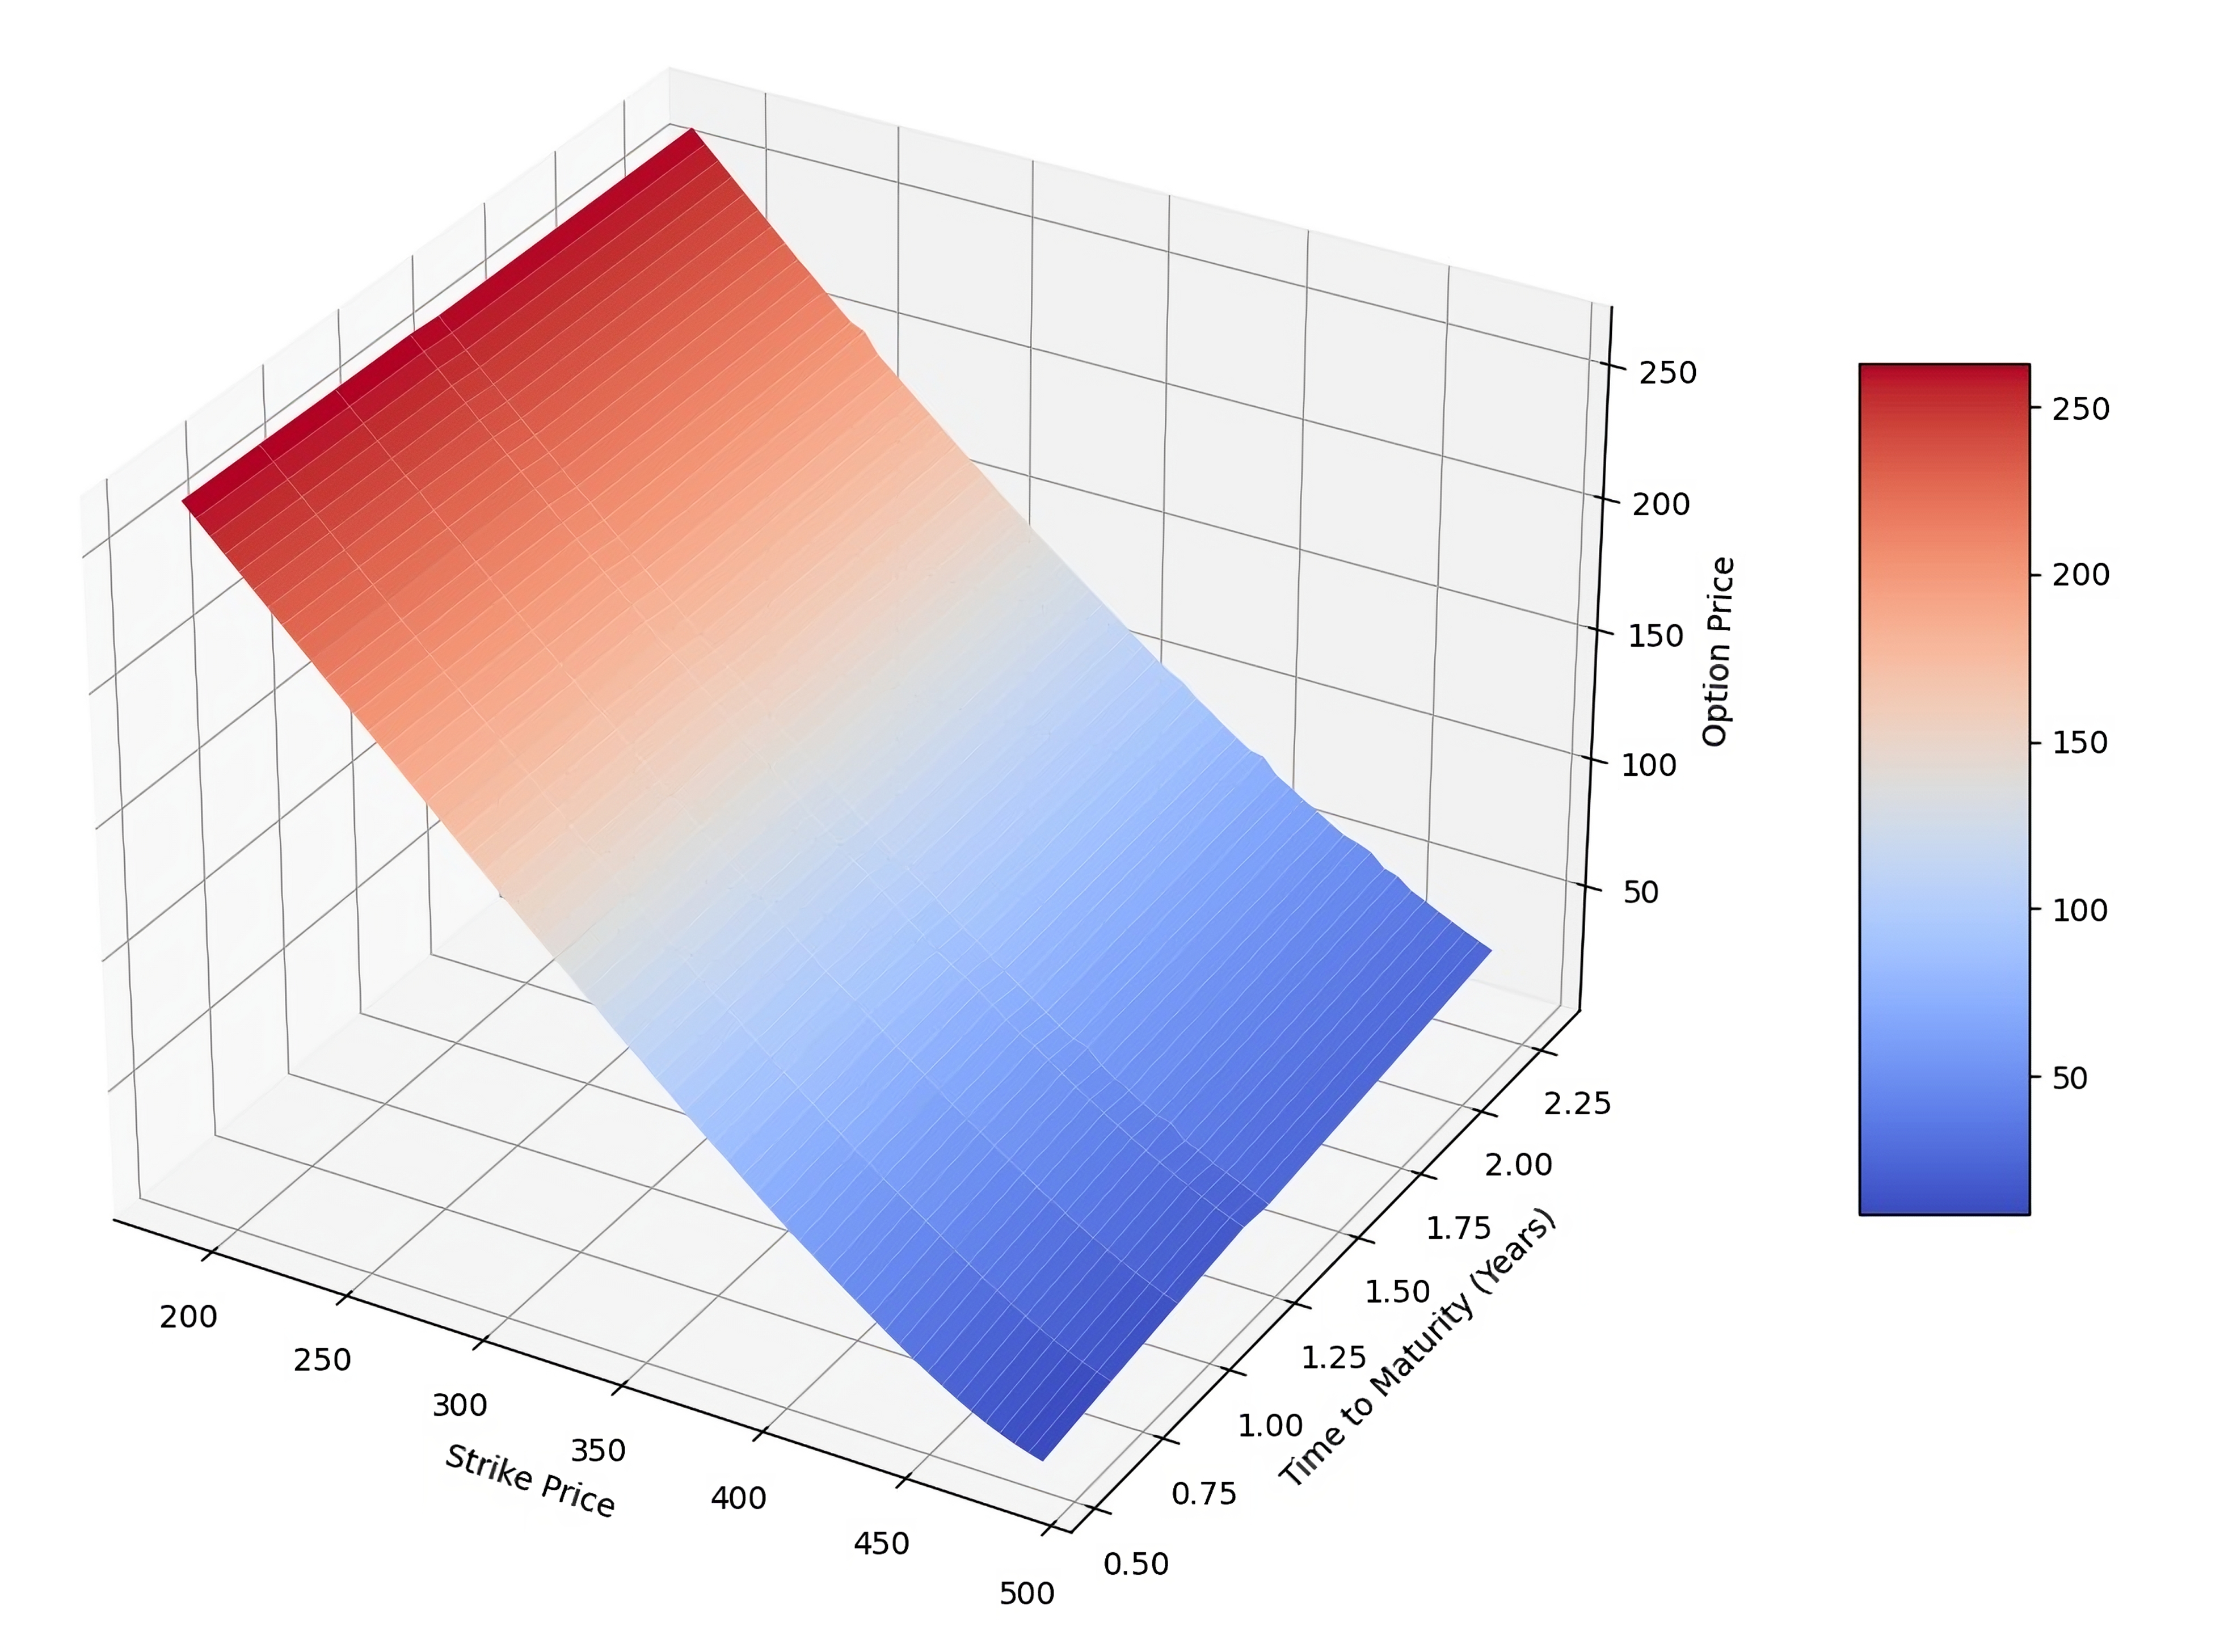
\includegraphics[width=1\textwidth]{Figure_OptionSurface.png}
		\caption{Γραφική παράσταση των διαθέσιμων δικαιωμάτων στην αγορά σε μία συγκεκριμένη ημερομηνία.}
		\label{fig:OptionSurface}
		\vspace{2mm}
	\end{figure}
	
\subsection{Μέθοδος εκτίμησης}
	\vspace{2.5mm}
	Όταν εκτιμούμε τις παραμέτρους του μοντέλου \selectlanguage{english}Heston\selectlanguage{greek}, πρέπει να λάβουμε υπόψη το γεγονός ότι έχουμε δικαιώματα με πολλές διαφορετικές ημερομηνίες λήξης $(T)$ και διαφορετικές τιμές εξάσκησης $(K)$. Οι παράμετροι $\kappa, \theta, \sigma, \rho, v_0$ πρέπει να αντιπροσωπεύουν όλο το σύνολο των δικαιωμάτων ή τουλάχιστον τα πιο σημαντικά δικαιώματα, για παράδειγμα αυτά των οποίων η τιμή εξάσκησης εμφανίζεται συχνά στην βάση δεδομένων. Επιπλέον, σε περίπτωση εισαγωγής νέων δεδομένων, οι παράμετροι δεν θα πρέπει να επηρεάζονται σημαντικά.
	\vspace{2.5mm}\\
	Θέλουμε η βάση δεδομένων να έχει την μορφή πίνακα ο οποίος θα περιέχει την τιμή ενός δικαιώματος για κάθε τιμή εξάσκησης και για κάθε ημερομηνία λήξης. Αυτός ο πίνακας έχει την μορφή πλέγματος οπότε μπορούμε να τον παραστήσουμε γραφικά σαν μια επιφάνεια (βλ. Σχήμα \eqref{fig:OptionSurface}).
	\vspace{2.5mm}\\
 	Για την εκτίμηση των παραμέτρων για τα δικαιώματα αγοράς (ομοίως και για δικαιώματα πώλησης), θα χρησιμοποιήσουμε την μέθοδο των ελάχιστων τετραγωνικών σφαλμάτων. Έστω $\Theta = (\kappa, \theta, \sigma, \rho, v_0, \lambda)$ οι άγνωστοι, $\{K_1,K_2,\dots,K_N\}$ ένα σύνολο που περιέχει τιμές εξάσκησης και $\{T_1,T_2,\dots,T_M\}$ ένα σύνολο που περιέχει ημερομηνίες λήξης. Ορίζουμε, $\sigma_{ij}$ η  διακύμανση \selectlanguage{english}(implied volatility)\selectlanguage{greek} που αντιστοιχεί σε ένα δικαίωμα με τιμή εξάσκησης $K_i$ και ημερομηνία λήξης $T_j$ (το μέτρο αυτό δίνεται απο το χρηματιστήριο και υπάρχει στα δεδομένα), τότε
 	\[SqErr(\Theta) = \sum_{i=1}^{N}\sum_{j=1}^{M}w_{ij}[C_{MP}(K_i,T_j) - C_{HP}(S(t),K_i,T_j,r_t,\Theta)]^2 + \text{\selectlanguage{english}Penalty}(\Theta,\Theta_0) \label{SqErr}\tag{4.3.1}\]
 	όπου
 	\begin{itemize}
 		\item $C_{MP}(K_i,T_j)$: η τιμή στο χρηματιστήριο του δικαιώματος αγοράς που έχει τιμή εξάσκησης $K_i$ και ημερονηνία λήξης $T_j$.
 		\item $C_{HP}(S(t),K_i,T_j,r_t,\Theta)$: η τιμή του δικαιώματος αγοράς που υπολογίστηκε χρησιμοποιώντας το μοντέλο \selectlanguage{english}Heston\selectlanguage{greek}, η οποία εξαρτάται από το διάνυσμα $\Theta$. Η παράμετρος $r_t$ δηλώνει το επιτόκιο μηδενικού ρίσκου.	
 	\end{itemize}
 	Μπορούμε να ορίσουμε $\text{\selectlanguage{english}Penalty}(\Theta,\Theta_0) = \norm{\Theta-\Theta_0}^2$, όπου $\Theta_0$ είναι οι αρχικές τιμές των παραμέτρων, αυξάνοντας την σταθερότητα του υπολογισμού των παραμέτρων. Για τα βάροι, μπορούμε να ορίσουμε $w_{ij}=\frac{1}{|bid_{ij}-ask_{ij}|}$. Αυτό σημαίνει ότι όταν η διαφορά μεταξύ των τιμών προσφοράς και ζήτησης για ένα δικαίωμα είναι μικρή τότε λαμβάνεται μεγαλύτερο βάρος, ενώ όταν υπάρχει μεγάλη διαφορά, λαμβάνεται μικρότερο βάρος. Ενναλλακτικά, μπορεί να χρησιμοποιειθεί και η \selectlanguage{english}implied volatility\selectlanguage{greek} κάθε δικαιώματος ως βάρος, καθώς αντικατοπτρίζει τις προσδοκίες της αγοράς για μελλοντικές διακυμάνσεις τιμών. Δηλαδή, $w_{ij}=\sigma_{ij}$.
 	\vspace{2.5mm}\\
 	Έχουμε ήδη αναφέρει ότι σύμφωνα με την μέθοδο \selectlanguage{english}Martingale\selectlanguage{greek}, οι τύποι για την αξία Αμερικάνιων δικαιωμάτων αγοράς και πώλησης είναι αντίστοιχα 
 	\[C(K_i,T_j) = \sup_{0\leq\tau\leq T_j}\mathbb{E}\left[e^{-r_j\tau}\max\{S(T)-K_i, 0\}\right] \quad\text{και}\quad 
 		P(K_i,T_j) = \sup_{0\leq\tau\leq T_j}\mathbb{E}\left[e^{-r_j\tau}\max\{K_i - S(T), 0\}\right] \]
 	όπου $\tau$ χρόνος εξάσκησης.
 
 \subsection{Μέθοδοι βελτιστοποίησης}
 	Στόχος μας είναι η εύρεση ελαχίστου για την συνάρτηση \eqref{SqErr} το οποίο είναι προφανώς ένα πρόβλημα μη γραμμικού προγραμματισμού. Μετά από δοκιμές, καταλήξαμε στο συμπέρασμα ότι η συνάρτηση δεν είναι κυρτή και περιέχει πολλά τοπικά ελάχιστα σημεία. Έτσι, αποφασίσαμε να εφαρμόσουμε την στοχαστική μέθοδο βελτιστοποίησης \selectlanguage{english}Simulated Annealing\selectlanguage{greek}\cite{SA 1}, \cite{SA 2} σε συνδυασμό με την  προσδιοριστική μέθοδο βελτιστοποίησης \selectlanguage{english}Trust Region Reflective\selectlanguage{greek}\cite{Method:Trust Region Reflective}.
 	\vspace{2.5mm}\\
 	Για την εφαρμογή τους θα χρησιμοποιήσουμε το πακέτο \selectlanguage{english}SciPy\selectlanguage{greek} της \selectlanguage{english}Python\selectlanguage{greek} που περιέχει την υλοποίηση και των δύο αλγορίθμων, όπως ακριβώς περιγράφεται στα \cite{Method:Trust Region Reflective}, \cite{SA 1}.
 	\begin{itemize}
 		\item Ντετερμινιστικοί (τοπικοί) αλγορίθμοι βελτιστοποίησης:\\
 			Η επιλογή του αρχικού σημείου (εδώ το $\Theta_0\in\mathbb{R}^6$) επηρεάζει σημαντικά την αποτελεσματικότητα τέτοιων αλγορίθμων. Από το αρχικό σημείο, υπολογίζεται η βέλτιστη διεύθυνση και το βήμα, ώστε να βρεθεί το ελάχιστο της συνάρτησης. Υπάρχουν πολλοί τέτοιοι αλγόριθμοι και αρκετοί από αυτούς συγκλίνουν σχετικά γρήγορα σε ελάχιστο, ωστόσο υπάρχει πάντα ο κίνδυνος να καταλήξουν σε τοπικό και όχι ολικό ελάχιστο. Επομένως, πρέπει να χρησιμοποιούνται όταν έχουμε ένα <<καλό>> αρχικό σημείο, για παράδειγμα όταν χρειάζεται να ξαναεκτιμήσουμε τις παραμέτρους του μοντέλου κάθε μέρα και οι τιμές δεν έχουν αλλάξει πολύ. 
 		\item Στοχαστικοί (ολικοί) μέθοδοι: \\
 			Η αρχική υπόθεση δεν έχει σημασία για την απόδοση των στοχαστικών μεθόδων βελτιστοποίησης, όπως είναι η \selectlanguage{english}simulated annealing\selectlanguage{greek}. Σε γενικές γραμμές, οι στοχαστικοί αλγόριθμοι τείνουν να έχουν μεγαλύτερο υπολογιστικό κόστος σε σύγκριση με τους ντετερμινιστικούς. Ο αλγόριθμος της \selectlanguage{english}simulated annealing\selectlanguage{greek} επιλέγει τυχαία την κατεύθυνση και το μέγεθος του βήματος, κινούμενος πάντα προς τα κάτω. Μπορεί να επιτρέπει περιστασιακές κινήσεις προς τα πάνω για να ξεφύγει από τοπικά ελάχιστα, με μια συγκεκριμένη πιθανότητα $P_T$, η οποία εξαρτάται από την παράμετρο $T$ (παραδοσιακά ονομάζεται παράμετρος θερμοκρασίας). Υπάρχουν κάποια θεωρήματα σύγκλισης που αποδεικνύουν ότι ο αλγόριθμος καταλήγει πάντα στο ολικό ελάχιστο, εφόσον η διαδικασία είναι αρκετά αργή.
 	\end{itemize}
 	Για την εκτίμηση των τιμών των δικαιωμάτων θα χρησιμοποιήσουμε συναρτήσεις που έχουμε ήδη αναφέρει όπως μια παραλλαγή της \selectlanguage{english}LSM\selectlanguage{greek} μεθόδου που βρίσκει την τιμή απλών Αμερικάνικων δικαιωμάτων, από το κεφάλαιο 3, και της \selectlanguage{english}HestonModelSim\selectlanguage{greek} την οποία είδαμε σε αυτό το κεφάλαιο. Η μόνη παραλλαγή είναι ότι τώρα αναγκαζόμαστε να χρησιμοποιήσουμε κλάσεις δεδομένων ώστε να εφαρμοστούν σωστά οι παραπάνω συναρτήσεις. Επιπλέον, θα συγκρίνουμε το μοντέλο του \selectlanguage{english}Heston\selectlanguage{greek} με το μοντέλο των \selectlanguage{english}Black-Scholes\selectlanguage{greek}, που δεν είναι άλλο παρά η γεωμετρική κίνηση \selectlanguage{english}Brown\selectlanguage{greek} με σταθερούς συντελεστές ($r_t \, ,\, \sigma_{ij}$), των οποίων η τιμή υπάρχει στα δεδομένα. Ο αναλυτικός κώδικας βρίσκεται στο κεφάλαιο 5.
 	\vspace{2.5mm}\\
 	Θα προσπαθήσουμε να βρούμε ένα σύνολο παραμέτρων, ξεκινώντας από την ημερομηνία 1-9-2021, το οποίο να ταιριάζει στα δεδομένα που είναι διαθέσιμα εκείνη την χρονική στιγμή. Ο βέλτιστος τρόπος για να επιτευχθεί αυτό είναι η εκτίμηση των παραμέτρων να γίνει πάνω σε δικαιώματα που διαπραγματεύονται περισσότερο στην αγορά. Θα κρατήσουμε δηλαδή, τα δικαιώματα που έχουν τιμή εξάσκησης η οποία εμφανίζεται σε κάθε διαθέσιμη ημερομηνία λήξης. Θα πάρουμε τον παρακάτω πίνακα με δείκτη σειράς τις μέρες έως την ημερομηνία λήξης (αρχική ημερομηνία 1-9-2021) και δείκτη στήλης τις συνήθεις τιμές εξάσκησης. Το στοιχείο $\alpha_{ij}$ του πίνακα αντιστοιχεί στην τιμή του δικαιώματος με ημερομηνία λήξης $T_i$ μέρες από <<σήμερα>> (1-9-2021) και τιμή εξάσκησης $K_j$. Όπως δείξαμε παραπάνω, μπορούμε να παραστήσουμε αυτόν τον πίνακα σαν μία επιφάνεια (βλ. Σχήμα \eqref{fig:OptionSurface}).
 	\begin{figure}[h]
 		\centering
 		\includegraphics[width=1\textwidth]{Figure_CommonStrikes.png}
 		\caption{Δεδομένα ενός έτους για συνήθεις δικαιώματα. Υπάρχουν 28 στήλες και 27 γραμμές, άρα συνολικά 756 διακεκριμένα δικαιώματα.}
 		\label{fig:CommonStrikes}
 		\vspace{2mm}
 	\end{figure}
 	
 	\noindent Για την εκτίμηση των παραμέτρων του μοντέλου \selectlanguage{english}Heston\selectlanguage{greek}, ξεκινάμε εφαρμόζοντας την μέθοδο \selectlanguage{english}simulated annealing\selectlanguage{greek}, βρίσκοντας έτσι μια λίστα υποψήφιων ολικών ελαχίστων. Έπειτα σε καθένα από αυτά τα σημεία εφαρμόζουμε την \selectlanguage{english}trust region reflective\selectlanguage{greek}. Με αυτό τον τρόπο βρίσκουμε το ολικό ελάχιστο (με λίγη τύχη) για την συνάρτηση \eqref{SqErr}
 	\[\Theta = (2.23889343, 0.05990061, 0.84803817, -0.28413532, 0.01142813, -0.21339978) \]
 	
 	\noindent Εναλλακτικά, ξεκινώντας με αρχική εκτίμηση (τυχαία) 
 	\[\Theta_0 = (\kappa_0, \theta_0, \sigma_0, \rho_0, v_{00}, \lambda_0) = (0.5 , 0.1, 0.1, 0.1, 0.1, 0) \]
 	η μέθοδος \selectlanguage{english}trust region reflective\selectlanguage{greek} έχει την δυνατότητα να καταλήξει σε ένα ικανοποιητικό τοπικό ελάχιστο ή ακομα και το ολικό ελάχιστο, με αρκετή τύχη.
 	
 \subsection{Αποτελέσματα}
 \vspace{2.5mm}	
 	Εφαρμόζοντας το μοντέλο με παραμέτρους $\Theta$, βλέπουμε απο τα σχήματα \ref{fig:SurfaceHeston}, \ref{fig:SurfaceBS} ότι προσεγγίζει σχετικά καλά τις πραγματικές τιμές τις αγοράς, έχοντας μέσο απόλυτο σχετικό σφάλμα $0.44\%$. Αξίζει να σημειωθεί ότι, πάνω στα ίδια δεδομένα, το μοντέλο των \selectlanguage{english}Black-Scholes\selectlanguage{greek} πέτυχε μέσο απόλυτο σχετικό σφάλμα $0.93\%$. 
 	\vspace{2.5mm}
 	\begin{center}
 		\begin{tabular}{|c|c|c|} 
 			\hline 
 			&\selectlanguage{english} Heston Model &\selectlanguage{english}Black-Scholes Model  \\
 			\hline
 			\selectlanguage{english}Average Absolute Error (\%)\selectlanguage{greek} & 0.44 & 0.93  \\
 			\hline
 			\selectlanguage{english}Mean Squared Error\selectlanguage{greek} & 0.194 & 1.17  \\
 			\hline
 			\selectlanguage{english}Total Squared Error\selectlanguage{greek} &116.41 & 341.83 \\
 			[0.5ex] 
 			\hline
 		\end{tabular}
 	\end{center}
 	\vspace{2.5mm}
 	\noindent Από τις εικόνες \ref{fig:RelErrorsWithHeston} και \ref{fig:RelErrorsWithBS} γίνεται ξεκάθαρο ότι το μοντέλο \selectlanguage{english}Black-Scholes\selectlanguage{greek} προσεγγίζει με μεγαλύτερο σφάλμα τις πραγματικές τιμές και τείνει να τις υπερεκτιμά (με μέγιστο σφάλμα περίπου $2.5\%$). Από την άλλη, το μοντέλο \selectlanguage{english}Heston\selectlanguage{greek} προσεγγίζει με μικρή διαφορά τις πραγματικές τιμές δικαιωμάτων που έχουν <<μικρή>> τιμή εξάσκησης. Οι μεγαλύτερες αποκλίσεις (σχεδόν όλες $<1\%$ με μέγιστο, $1.48\%$) εμφανίζονται στα δικαιώματα με ημερομηνία λήξης πάνω από ένα έτος.
 	\vspace{2.5mm}\\
 	\noindent Προσωμοιώσαμε την υποκείμενη τιμή του περιουσιακού στοιχείου 10.000 φορές για κάθε αποτίμηση δικαιώματος ώστε να λάβουμε αυτά τα αποτελέσματα. Οι 10.000 επαναλήψεις φαίνεται να είναι το ιδανικό σημείο μεταξύ ακρίβειας και χρόνου. Η μέθοδος \selectlanguage{english}TRF\selectlanguage{greek} αποδείχθηκε αρκετά αξιόπιστη όταν υπάρχει ένα <<καλό>> αρχικό σημείο. Τα αποτελέσματα μπορούν να βελτιωθούν αν για παράδειγμα αντί για την μέθοδο διακριτοποίησης \selectlanguage{english}Euler\selectlanguage{greek}, εφαρμόζαμε αυτή του \selectlanguage{english}Milstein\selectlanguage{greek} \cite{EulerDiscr} και πραγματοποιώντας περισσότερες προσομοιώσεις. Οι ίδιες παράμετροι του μοντέλου, θεωρητικά, μπορούν να χρησιμοποιηθούν ώστε να εκτιμήσουμε και την αξία δικαιωμάτων πώλησης.
 	
 	\begin{figure}[h]
 		\begin{minipage}[b]{0.5\linewidth}
 			\centering
 			\includegraphics[width=\linewidth]{MarketSurfaceHeston1.png}
 			\caption{Προσεγγίσεις με το μοντέλο\\ \selectlanguage{english}Heston\selectlanguage{greek}}
 			\label{fig:SurfaceHeston}
 		\end{minipage}
 		\hspace{0.02\linewidth}  % Horizontal space between images
 		\begin{minipage}[b]{0.5\linewidth}
 			\centering
 			\includegraphics[width=\linewidth]{MarketSurfaceBS1.png}
 			\caption{Προσεγγίσεις με το μοντέλο \selectlanguage{english}Black-Scholes\selectlanguage{greek}}
 			\label{fig:SurfaceBS}
 		\end{minipage}
 	\end{figure}
 	
 	\begin{figure}[h]
 		\centering
 		\includegraphics[width=1\textwidth]{Heston Model RelErrors Sides.png}
 		\caption{Σχετικά λάθη μετά την εκτιμήση με το μοντέλο \selectlanguage{english}Heston\selectlanguage{greek}.}
 		\label{fig:RelErrorsWithHeston}
 	\end{figure}
 	\clearpage
 	
 	
 	\begin{figure}[h]
 		\centering
 		\includegraphics[width=1\textwidth]{BS Model RelErrors0.9.png}
 		\caption{Σχετικά λάθη μετά την εκτιμήση με το μοντέλο \selectlanguage{english}Black-Scholes\selectlanguage{greek}.}
 		\label{fig:RelErrorsWithBS}
 		\vspace{4mm}
 	\end{figure}
 	
 	
 	\noindent Ένας τρόπος να επιταχύνουμε σημαντικά την εκτίμηση παραμέτρων στην περίπτωση του Αμερικάνικου δικαιώματος αγοράς, είναι αντί για προσομοιώσεις \selectlanguage{english}Monte-Carlo\selectlanguage{greek}, να χρησιμοποιήσουμε τον αναλυτικό τύπο για την αποτίμηση Ευρωπαϊκών δικαιωμάτων αγοράς, ο οποίος μπορεί να βρεθεί αναλυτικά στο \cite{Heston} (βλ. Κεφάλαιο 5 για υλοποίηση στην \selectlanguage{english}Python\selectlanguage{greek}).
 	
 	\begin{table}[t]
 		\centering
 		\begin{tabular}{|c|c|c|} 
 			\hline 
 			& \selectlanguage{english}Monte-Carlo simulations  & \selectlanguage{english}Closed-form solution \\ % This breaks the header into two lines
 			\hline
 			\selectlanguage{english}Average Absolute Error (\%)\selectlanguage{greek} & 0.44 & 0.52  \\ 
 			\hline
 			\selectlanguage{english}Mean Squared Error\selectlanguage{greek} & 0.194 & 0.222  \\ 
 			\hline
 			\selectlanguage{english}Total Squared Error\selectlanguage{greek} & 116.41 & 133.42 \\ 
 			[0.5ex] 
 			\hline
 		\end{tabular}
 		\caption{Αποτελέσματα από δύο μεθόδους εκτίμησης παραμέτρων για το μοντέλο \selectlanguage{english}Heston\selectlanguage{greek}. Παρατηρούμε ότι δεν διαφέρουν πολύ τα αποτελέσματα, πράγμα λογικό καθώς το \selectlanguage{english}ETF SPY\selectlanguage{greek} πληρώνει σχετικά μικρό ποσό μερίσματος (επιστροφή περίπου $1.2\%$) κάθε 3 μήνες}. 
 	\end{table}
 	
 	\noindent Εφαρμόζοντας αυτές τις διαφορετικές μεθόδους έτυχε και τα διανύσματα $\Theta$ στις δύο περιπτώσεις να είναι παρόμοια.
 	\vspace{2.5mm}\\
 	\noindent Έτσι, η στοχαστική μέθοδος δίνει πολύ γρηγορότερα τα υποψήφια ολικά ελάχιστα. Συνεχίζουμε εφαρμόζοντας την ντετερμινιστική μέθοδο (τώρα με προσομοιώσεις \selectlanguage{english}Monte-Carlo\selectlanguage{greek}), ώστε να βρούμε το βέλτιστο σημείο. Αυτή η <<παράτυπη>> μέθοδος μπορεί να λειτουργήσει καθώς, όπως προαναφέραμε, στην περίπτωση μετοχών που δεν πληρώνουν μέρισμα, το Αμερικάνικο δικαίωμα αγοράς και το Ευρωπαϊκό έχουν ίδια αξία (δεδομένου προφανώς ότι έχουν ίδια ημερομηνία λήξης και τιμή εξάσκησης). Η πληρωμή μερίσματος μειώνει την τιμή του υποκείμενου περιουσιακού στοιχείου, καθώς τότε, η συνολική αξία της εταιρείας μειώνεται κατά το ποσό του μερίσματος. Αυτή η μείωση στην αξία αντανακλάται στην τιμή της μετοχής. Για τα δικαίωματα αγοράς, η πληρωμή μερίσματος μπορεί να μειώσει την ελκυστικότητα της κατοχής του δικαιώματος, καθώς η τιμή της μετοχής θα πέσει μετά την ημερομηνία πληρωμής μερίσματος, ενώ για τα δικαιώματα πώλησης, η πτώση της τιμής μπορεί να τα κάνει πιο πολύτιμα, καθώς η τιμή της υποκείμενης μετοχής μειώνεται.
 	
 
 	
 	
\chapter*{Επίλογος}
	 	Ως μαθηματικοί (ή φοιτητές μαθηματικών), μπορούμε να παρασυρθούμε από τη μαγεία των Μαθηματικών. Είναι σημαντικό να θυμόμαστε ότι το μοντέλο \selectlanguage{english}Heston\selectlanguage{greek} είναι, ουσιαστικά, ένα μοντέλο. Είναι ένα μαθηματικό εργαλείο που προσομοιώνει κάτι απείρως πολύπλοκο. Ως εκ τούτου, δεν μπορεί να αποτυπώσει πλήρως τη σύνθετη και ποικιλόμορφη δυναμική που υπάρχει στην πραγματικότητα όσον αφορά τη μεταβλητότητα.
	 	\vspace{2.5mm}\\
	 	\noindent Η εκτίμηση των παραμέτρων του μοντέλου είναι μια σημαντική εργασία. Ωστόσο, δεν πρέπει να σπαταλιέται ενέργεια στην υπερβολική προσαρμογή του μοντέλου \selectlanguage{english}(overfitting)\selectlanguage{greek}. Τέτοιες προσπάθειες μπορεί να οδηγήσουν σε παραπλανητικά αποτελέσματα. Εξάλλου, προσπαθούμε να προσαρμόσουμε τέλεια ένα μοντέλο που δεν εξηγεί τέλεια τον πραγματικό κόσμο.
	 	\vspace{2.5mm}\\
	 	\noindent Αυτό δεν καθιστά, γενικά, τα στοχαστικά μοντέλα άχρηστα. Αν κατανοηθούν προσεκτικά οι υποθέσεις και εφαρμοστούν με προσοχή, τότε τα στοχαστικά μοντέλα είναι ισχυρά εργαλεία. Είναι ό,τι καλύτερο έχουμε σε έναν απρόβλεπτο κόσμο, χωρίς τα οποία θα ήμασταν πολύ χειρότερα.
 	
 	
 	
 	
 	
\chapter*{Κώδικας στην \selectlanguage{english}Python}
\raggedright
	Σε αυτό το κεφάλαιο παρουσιάζουμε τον κώδικα που αναπτύξαμε για την δημιουργία των εικόνων του κειμένου και για την επίλυση εξίσωσεων.
	\vspace{2.5mm}\\ 
	Θα χρειαστούμε τις βιβλιοθήκες της \selectlanguage{english}Python:
	\vspace{4mm}
\begin{lstlisting}
 import numpy as np
 import matplotlib.pyplot as plt 
 #To use latex syntax (optional)
 plt.rcParams.update({'mathtext.default': 'regular'})  \end{lstlisting}
 	\vspace{4mm}
 	\selectlanguage{greek}
 	Για την εικόνα (\ref{fig:SymmRndWalk}) στην σελίδα \pageref{fig:SymmRndWalk}:
 	\selectlanguage{english}
 	\vspace{4mm}
\begin{lstlisting}
 def RandomWalkSim(M, t):      # M = number of simulations, t = time
 	# Possible steps in the random walk (array)
 	random_walk= [-1, 1]
 	# txM matrix where every column represents a random walk
 	steps= np.random.choice(random_walk, size=(t, M)) 
 	# 1xM array of zeroes, represents the starting position
 	origin= np.zeros((1,M)) 
 	rw_paths= np.concatenate([origin, steps]).cumsum(axis=0)
 		
 	# Create points for every position of the random walk (optional)
 	for i in range(M):
 		plt.plot(range(t + 1), rw_paths[:, i], marker='o', 
 				 color= "black", label=f'Walk {i + 1}')
 		# Name those point (here we use latex syntax) 
 		for x, y in zip(range(t + 1), rw_paths[:, i]):
 			plt.text(x, y, f'$M_{x}$', color='black', fontsize=10, 
 					 ha='left', va='bottom')
 	# Set y-axis ticks to integers
 	plt.yticks(range(int(min(rw_paths.min(), -1)) - 1, 
 						     int(max(rw_paths.max(), 1)) + 2))  
 						     				        		
 	plt.plot(rw_paths)
 	plt.xlabel("Time (t)")
 	plt.ylabel("Position")
 	plt.title("Symmetric Random Walk")
 	plt.show()\end{lstlisting}
 	\vspace{4mm}
 	\selectlanguage{greek}
 	Για την εικόνα (\ref{fig:ScaledRndWalk}) στην σελίδα \pageref{fig:ScaledRndWalk}:
 	\selectlanguage{english}
 	\vspace{4mm}
\begin{lstlisting}
 def SccaledRandomWalkSim(M, t, n): 
 	# M = number of simulations, t = time, n = steps
 	random_walk= [-1, 1]
 	steps= (1/np.sqrt(n))*np.random.choice(random_walk, size=(t*n, M))
 	origin= np.zeros((1, M))
 	srw_paths= np.concatenate([origin, steps]).cumsum(axis=0)
 		
 	# Define time interval correctly:
 	# array of t*n+1 evenly spaced values over the interval [0, t]
 	time= np.linspace(0, t, t*n + 1)  
 	# Requiere numpy array that has the same shape as srw_paths
 	tt= np.full(shape=(M, t*n + 1), fill_value=time).T
 		
 	plt.plot(tt, srw_paths)
 	plt.xlabel("Time (t)")
 	plt.ylabel("Position")
 	plt.title("Scaled Random Walk")
 	plt.show() \end{lstlisting}
 	\vspace{4mm}
 	\selectlanguage{greek}
 	Για την εικόνα (\ref{fig:Binomial}) στην σελίδα \pageref{fig:Binomial}:
 	\selectlanguage{english}
 	\vspace{4mm}
\begin{lstlisting}
 def BintoNormal(n, t):
 	# Calculate the probabilities of different outcomes 
 	# in a binomial distribution Bin(nt, 0.5)
 	probs= [stats.binom.pmf(k, n*t, 0.5) for k in range(int(n*t)+1)]
 		
 	# Generate the outcomes of a scaled random walk
 	outcomes= 1/np.sqrt(n) * np.arange(-n*t, n*t+1, 2) 
 		
 	# Plot the binomial distribution, normalizing each probability
 	plt.bar(outcomes, 
 	      height=[prob/(outcomes[1]-outcomes[0]) for prob in probs], 
 		  width=outcomes[1] - outcomes[0], label=f'{n} scaled RW')
 		
 	# Plot the normal distribution
 	x = np.linspace(-3*np.sqrt(t), 3*np.sqrt(t), 100)  
 	plt.plot(x, stats.norm.pdf(x, 0, np.sqrt(t)), 'k-', 
 			 label='normal dist')    
 		
 	# Set plot limits and labels
 	plt.xlim(-3.5*np.sqrt(t), 3.5*np.sqrt(t))
 	plt.ylabel("Probability")
 	plt.xlabel("Move")
 		
 	# Show legend and plot
 	plt.legend()
 	plt.show()\end{lstlisting}
 	\vspace{4mm}
 	\selectlanguage{greek}
 	Για την εικόνα (\ref{fig:Brown}) στην σελίδα \pageref{fig:Brown}:
 	\selectlanguage{english}
 	\vspace{4mm}
\begin{lstlisting}
 def BrownianMotionSim(M, t, n):  
 	# M= number of simulations, t = time, n = steps
 	dt= t / n  # time step
 	steps = np.sqrt(dt) * np.random.normal(0, 1, size=(n, M))
 	origin= np.zeros((1, M))  # 1xM array of zeroes
 	bm_paths= np.concatenate([origin, steps]).cumsum(axis=0)
 		
 	# Define time interval correctly:
 	# array of n+1 evenly spaced values over the interval [0, t]
 	time= np.linspace(0, t, n + 1)  
 	# Requiere numpy array that has the same shape as bm_paths
 	tt= np.full(shape=(M, n+1), fill_value=time).T
 		
 	plt.plot(tt, bm_paths, linewidth=0.8)
 	plt.xlabel("Time (t)")
 	plt.ylabel("Position")
 	plt.title("Brownian Motion")
 	plt.show() \end{lstlisting}
 	\vspace{4mm}
 	\selectlanguage{greek}
 	Για την εικόνα (\ref{fig:ReflectedBM}) στην σελίδα \pageref{fig:ReflectedBM}:
 	\selectlanguage{english}
 	\vspace{4mm}
\begin{lstlisting}
 def BrownianMotionSimWithReflection(t, n, reflection_time):
 	dt= t / n  # time step
 	steps = np.sqrt(dt) * np.random.normal(0, 1, size=(n, 1))
 	origin= np.zeros((1, 1))  # 1x1 array of zeroes
 	bm_paths= np.concatenate([origin, steps]).cumsum(axis=0)
 		
 	# Reflect paths after a certain time
 	reflection_index= int(reflection_time / t * n)
 	reflected_steps= steps[reflection_index:]
 	reflected_origin= bm_paths[reflection_index-1:reflection_index]
 	reflected_paths= np.concatenate(
 			    [reflected_origin, -reflected_steps]).cumsum(axis=0)
 		
 	# Define time interval correctly, 
 	# here we don't need tt because M=1
 	# Array of n+1 evenly spaced values over the interval [0, t]
 	time = np.linspace(0, t, n + 1)  
 		
 	# Plot both paths on the same time axis
 	plt.plot(time, bm_paths, 'k-', label="Original Path")
 	plt.plot(time[reflection_index:], reflected_paths, 'r-',
 			 label="Reflected Path")
 	# Plot a line highlighting the symmetry
 	plt.axhline(y=reflected_origin[0,0], ls="- -", c="black")
 	# Ommit the values of y-axis and add only the point m 
 	plt.yticks([reflected_origin[0, 0]], ["m"])
 	# Alternatively add m as a value on the y-axis
 	# plt.yticks(list(plt.yticks()[0]) + [reflected_origin[0, 0]])
 	# Ommit the values of x-axis and add only the point \tau_m
 	plt.xticks([time[reflection_index]], ["$\\tau_{m}$"])
 		
 	plt.xlabel("Time (t)")
 	plt.ylabel("Position")
 	plt.title("Brownian Motion with Reflection")
 	plt.legend()
 	plt.show() \end{lstlisting}
 	\vspace{4mm}
 	\selectlanguage{greek}
 	Για την εικόνα (\ref{fig:BMandMax}) στην σελίδα \pageref{fig:BMandMax}:
 	\selectlanguage{english}
 	\vspace{4mm}
\begin{lstlisting}
 def BrownianMotionSimWithMax(M, t, n):
 	dt = t / n  # time step
 	steps = np.sqrt(dt) * np.random.normal(0, 1, size=(n, M))
 	origin = np.zeros((1, M))  # 1xM array of zeroes
 	bm_paths = np.concatenate([origin, steps]).cumsum(axis=0)
 	# Compute running maximum at each time step
 	running_max = np.maximum.accumulate(bm_paths, axis=0)
 	# Define time interval correctly
 	time = np.linspace(0, t, n + 1)  
 	tt = np.full(shape=(M, n + 1), fill_value=time).T
 	# Plot Brownian motion paths
 	plt.plot(tt, bm_paths, 'k-', label='Brownian Motion')	
 	# Plot running maximum paths
 	plt.plot(tt, running_max, 'r--', label='Running Maximum')
 		
 	plt.xlabel("Time (t)")
 	plt.ylabel("Position")
 	plt.title("Brownian Motion with its Running Maximum")
 	plt.legend()
 	plt.show() \end{lstlisting}
 	\vspace{4mm}
 	\selectlanguage{greek}
 	Για την εικόνα (\ref{fig:GBM}) στην σελίδα \pageref{fig:GBM}:
 	\selectlanguage{english}
 	\vspace{4mm}
\begin{lstlisting}
 def GeomBrownianMotionSim(mu, M, T, n, S0, sigma):
 	# mu = drift M = number of simulations, t = time, n = steps, 
 	#S0 = initial stock price, sigma = volatility
 	# Calculate each time step
 	dt = T / n
 	St = np.exp(
 		 (mu - sigma ** 2 / 2) * dt
 		 + sigma 
 		 np.sqrt(dt) * np.random.normal(0, 1, size=(n, M)) )
 	# Vertically stack a row of ones in the array St
 	St = np.vstack([np.ones(M), St])  
 	St = S0 * St.cumprod(axis=0)
 		
 	# Plot the simulations
 	# Define time interval correctly
 	time = np.linspace(0, T, n + 1)
 	# Require numpy array that is the same shape as St
 	tt = np.full(shape=(M, n + 1), fill_value=time).T
 	plt.plot(tt, St, linewidth=0.8, label='Brownian Motion')
 	plt.xlabel("Time $(t)$")
 	plt.ylabel("Value $(S_t)$")
 	plt.title(
 		"Simulated GBM\n $dS_t = \mu S_t dt + \sigma S_t dW_t$
 		\n $S_0= {0}, \mu= {1}, \sigma= {2}$".format(S0,mu,sigma))
 	plt.show()\end{lstlisting}
 	\vspace{4mm}
 	\selectlanguage{greek}
 	Για την εικόνα (\ref{fig:HestonModel}) την σελίδα \pageref{fig:HestonModel}:
 	\selectlanguage{english}
 	\vspace{4mm} 	
\begin{lstlisting}
 def HestonModelSim(S0, v0, rho, kappa, theta, sigma, r, T, n, M):
 	# Define time interval
	dt = T / n
	# Arrays for storing prices and variances
	S = np.full(shape=(n + 1, M), fill_value=S0)
	v = np.full(shape=(n + 1, M), fill_value=v0)
	# Generate correlated brownian motions
	Z_v = np.random.normal(0, 1, size=(n, M))
	Z_s = rho * Z_v + np.sqrt(1 - rho ** 2) * 
		np.random.normal(0, 1, size=(n, M))
	
	for i in range(1, N + 1):
	S[i] = S[i - 1] * np.exp(
		(r - 0.5 * v[i - 1]) * dt + np.sqrt(v[i - 1] * dt) * 
		Z_s[i - 1,:])
	v[i] = np.maximum(
		v[i - 1] + kappa * (theta - v[i - 1]) * dt + 
		sigma * np.sqrt(v[i - 1] * dt) * Z_v[i - 1,:], 0)
	return S, v 

 def PlotHestonModel(S, v, T, N):
	fig = plt.figure(figsize=(12, 5))
	ax1 = fig.add_subplot(1, 2, 1)
	ax2 = fig.add_subplot(1, 2, 2)
	time = np.linspace(0, T, N + 1)
	
	ax1.plot(time, S)
	ax1.set_title('Heston Model Asset Prices')
	ax1.set_xlabel('Time')
	ax1.set_ylabel('Asset Prices')
	
	ax2.plot(time, v)
	ax2.set_title('Heston Model Variance Process')
	ax2.set_xlabel('Time')
	ax2.set_ylabel('Variance')
	
	plt.show()\end{lstlisting}
	\vspace{4mm}
	\selectlanguage{greek}
	Για την εικόνές (\ref{fig:VolSurRhos}), (\ref{fig:VolSurSigmas}) στις σελίδες \pageref{fig:VolSurRhos}, \pageref{fig:VolSurSigmas}:
	\selectlanguage{english}
	\vspace{4mm} 
\begin{lstlisting}
 import numpy as np
 import matplotlib.pyplot as plt
 from scipy.integrate import quad
 from scipy.stats import norm
 from scipy.optimize import brentq
 
 def BSimpvol(S, K, r, T, C):
 	"""
 	Calculate the implied volatility using the Black-Scholes model.
 	
 	Parameters:
 	S : float
 	Current stock price.
 	K : float
 	Strike price of the option.
 	r : float
 	Risk-free interest rate (annualized).
 	T : float
 	Time to maturity in years.
 	C : float
 	Price of the European call option.
 	
 	Returns:
 	float
 	Implied volatility.
 	"""
 	
 	# Initial guess for volatility
 	sigma = 0.2
 	
 	# Define the function to minimize
 	def f(sigma):
 		d1 = (np.log(S / K) + (r + 0.5 * sigma ** 2) * T) / (sigma * np.sqrt(T))
 		d2 = d1 - sigma * np.sqrt(T)
 		C_calc = S * norm.cdf(d1) - K * np.exp(-r * T) * norm.cdf(d2)
 		return C_calc - C
 	
 	# Use a numerical method to find the root
 	from scipy.optimize import brentq
 	
 	try:
 		implied_vol = brentq(f, 1e-6, 5.0)  # Find the root in the interval [1e-6, 5.0]
 		return implied_vol
 	except ValueError:
 		# If brentq fails, return NaN
 		return np.nan
 
 """Use Heston call pricing functions provided in this chapter"""
 
 # Define parameters
 kappa = 2
 theta = 0.05
 sigma = 0.2
 v0 = 0.08
 r = 0.02
 s0 = 100
 # Define strikes and maturities
 strikes = np.linspace(80, 120, 20)
 mats = np.linspace(0.3, 2, 20)  # maturities
 # Initialize price and volatility matrices
 prices = np.zeros((20, 20))
 Volatility = np.zeros((20, 20))
 
 
 """Plot volatility surface with changing rho"""
 # All together plots
 # Create a single figure for all surfaces
 fig = plt.figure(figsize=(18, 12))
 
 # First surface for rho = 0.5
 ax1 = fig.add_subplot(131, projection='3d')
 for i in range(20):
 	for j in range(20):
 		price = HestonCallQuad(
 			kappa,theta,sigma,0.5,v0,r,T=mats[i],s0=s0,K=strikes[j])
 		prices[i, j] = price
 		Volatility[i, j] = BSimpvol(s0, strikes[j], r, mats[i], price)
 
 # Create meshgrid for strikes and maturities
 strike, mat = np.meshgrid(strikes, mats)
 
 ax1.plot_surface(mat, strike, Volatility, cmap='coolwarm')
 ax1.set_xlabel('Maturity (years)')
 ax1.set_ylabel('Strike')
 ax1.set_title(r'$\rho = 0.5$')
 ax1.set_zlabel('Implied Volatility')
 
 # Second surface for rho = 0
 ax2 = fig.add_subplot(132, projection='3d')
 for i in range(20):
 	for j in range(20):
 		price = HestonCallQuad(
 			kappa,theta,sigma,0,v0,r,T=mats[i],s0=s0,K=strikes[j])
 		prices[i, j] = price
 		Volatility[i, j] = BSimpvol(s0, strikes[j], r, mats[i], price)
 
 ax2.plot_surface(mat, strike, Volatility, cmap='coolwarm')
 ax2.set_xlabel('Maturity (years)')
 ax2.set_ylabel('Strike')
 ax2.set_title(r'$\rho = 0$')
 ax2.set_zlabel('Implied Volatility')
 
 # Third surface for rho = -0.5
 ax3 = fig.add_subplot(133, projection='3d')
 for i in range(20):
 		for j in range(20):
 			price = HestonCallQuad(
 				kappa,theta,sigma,-0.5,v0,r,T=mats[i],s0=s0,K=strikes[j])
 			prices[i, j] = price
 			Volatility[i, j] = BSimpvol(s0, strikes[j], r, mats[i], price)
 
 ax3.plot_surface(mat, strike, Volatility, cmap='coolwarm')
 ax3.set_xlabel('Maturity (years)')
 ax3.set_ylabel('Strike')
 ax3.set_title(r'$\rho = -0.5$')
 ax3.set_zlabel('Implied Volatility')
 
 # Adjust layout and show
 plt.tight_layout()
 plt.show()
 
 
 """See how sigma (vol of vol) affects the volatility surface"""
 # Plot all together
 # Create a 1x3 grid of subplots (3 plots side by side)
 fig, axs = plt.subplots(1, 3, figsize=(18, 6))
 
 strikes = np.linspace(70, 130, 20)
 volvols = np.arange(0.1, 0.5, 0.1) # Volatility of volatility
 mats = np.linspace(0.3, 2, 20)  # maturities
 styles = ['-', '--', '-.', ':']
 colors = ['k', 'b', 'r', 'm']
 
 # Initialize price and volatility arrays
 prices = np.zeros((4, 20))
 Volatility = np.zeros((4, 20))
 
 # Rho values
 rho_values = [0.5, 0, -0.5]
 titles = ['rho = 0.5', 'rho = 0', 'rho = -0.5']
 
 # Iterate over the subplots and rho values
 for idx, rho in enumerate(rho_values):
 	# Plot for each rho
 	for i, sigma in enumerate(volvols):
 		for j, strike in enumerate(strikes):
 			price = HestonCallQuad(
 				kappa, theta, sigma, rho, v0, r, 
 				T=mats[i], s0=s0, K=strikes[j])
 			prices[i, j] = price
 			Volatility[i, j] = BSimpvol(s0, strikes[j], r, mats[i], price)
 
 		axs[idx].plot(strikes, Volatility[i, :], color=colors[i], 
 			linestyle=styles[i], label=f'sigma = {sigma:.1f}')
 
 		# Customize the subplot
 		axs[idx].set_ylabel('Implied Volatility')
 		axs[idx].set_xlabel('Strike')
 		axs[idx].set_title(titles[idx])
 		axs[idx].legend()
 
 # Adjust layout and show the plots
 plt.tight_layout()
 plt.show()\end{lstlisting}	
	\vspace{4mm}  	
	\selectlanguage{greek}
 	Για τον υπολογισμό της αξίας απλών Ευρωπαϊκών δικαιωμάτων με τον τύπο των \selectlanguage{english}Black-Scholes\selectlanguage{greek} \eqref{OptionCallFormula} και \eqref{OptionPutFormula}, χρησιμοποιήσαμε τον αλγόριθμο:
 	\selectlanguage{english}
 	\vspace{4mm}
\begin{lstlisting}
 import scipy.stats
 
 def PriceBS(S0, K, r, T, sigma, call_or_put= 'c'):
 	N = scipy.stats.norm.cdf
 	d1 = (np.log(S0/K) + (r+sigma**2/2)*T) / (sigma*np.sqrt(T))
 	d2 = d1 - sigma * np.sqrt(T)
 	if call_or_put == 'c':
 		return N(d1) * S0 - N(d2) * K * np.exp(-r*T)
 	elif call_or_put == 'p':
 		return N(-d2) * K * np.exp(-r*T) - N(-d1) * S0
 	else:
 		return "Specify call or put options." \end{lstlisting}
 	\vspace{4mm}
 	\selectlanguage{greek}
 	Για τον υπολογισμό της αξίας απλών Ευρωπαϊκών δικαιωμάτων αγοράς όταν η τιμή του υποκείμενου αγαθού ακολουθεί το μοντέλο του \selectlanguage{english}Heston\selectlanguage{greek} \eqref{HestonSDE} όπως περιγράφεται στο \cite{Heston}:
 	\selectlanguage{english}
 \begin{lstlisting}
 import numpy as np
 from scipy.integrate import quad
 
 def HestonCallQuad(kappa, theta, sigma, rho, v0, r, T, s0, K):
 """Computes the price of a European call option using the Heston model."""
 	call = s0 * HestonP(kappa, theta, sigma, rho, v0, r, T, s0, K, 1) \
 		- K * np.exp(-r * T) * 
 		HestonP(kappa, theta, sigma, rho, v0, r, T, s0, K, 2)
 	return call
 
 def HestonP(kappa, theta, sigma, rho, v0, r, T, s0, K, option_type):
 """Computes the characteristic function using numerical integration."""
 	integral_result = quad(HestonPIntegrand, 0, 100, 
 		args=(kappa, theta, sigma, rho, v0, r, T, s0, K, option_type))[0]
 	return 0.5 + (1 / np.pi) * integral_result
 
 def HestonPIntegrand(phi, kappa, theta, sigma, rho, v0, r, T, s0, K, 
 	option_type):
 """Evaluates the integrand for the Heston characteristic function."""
 	return np.real(np.exp(-1j * phi * np.log(K)) *
 		HestonCharfun(phi, kappa, theta, sigma, rho, v0, r, T, s0, 
 		option_type) / (1j * phi))
 
 def HestonCharfun(phi, kappa, theta, sigma, rho, v0, r, T, s0, 
 	option_type):
 """Computes the Heston characteristic function."""
 	if option_type == 1:
 	u = 0.5
 	b = kappa - rho * sigma
 	else:
 	u = -0.5
 	b = kappa
 
 	a = kappa * theta
 	x = np.log(s0)
 	d = np.sqrt((rho * sigma * phi * 1j - b)**2 - 
 		sigma**2 * (2 * u * phi * 1j - phi**2))
 	g = (b - rho * sigma * phi * 1j + d) / (b - rho * sigma * phi * 1j - d)
 
 	C = r * phi * 1j * T + (a / sigma**2) * 
 		((b - rho * sigma * phi * 1j + d) * T -
 		2 * np.log((1 - g * np.exp(d * T)) / (1 - g)))
 	D = (b - rho * sigma * phi * 1j + d) / sigma**2 *
 		 ((1 - np.exp(d * T)) / (1 - g * np.exp(d * T)))
 
 	return np.exp(C + D * v0 + 1j * phi * x)
 	
 # Example usage
 # Define parameters
 kappa = 2
 theta = 0.05
 sigma = 0.2
 rho = 0.5
 v0 = 0.08
 r = 0.02
 s0 = 100
 K = 110
 T = 1

 price = HestonCallQuad(kappa, theta, sigma, rho, v0, r, T, s0, K)
 print(price)\end{lstlisting}
 	\vspace{4mm}
 	\selectlanguage{greek}
 	Η εφαρμογή στον δείκτη \selectlanguage{english}S\&P 500\selectlanguage{greek} έγινε με τις εξής συναρτήσεις:
 	\selectlanguage{english}
 	\vspace{4mm}	
 \begin{lstlisting}
 import numpy as np
 import pandas as pd
 from dataclasses import dataclass
 from abc import ABC, abstractmethod	
 from scipy import optimize
 
 class StochasticProcess(ABC):
 	"""Represents a Stochastic process"""
 
 	@abstractmethod
 	def simulate(self):
 	...
 
 @dataclass
 class GeometricBrownianMotion(StochasticProcess):
 
 	mu: float
 	sigma: float
 	
 	def simulate(
 		self, s0: float, T: int, N: int, M: int, v0: float = None
 	) -> pd.DataFrame:  
 	# M = number of paths, N = number of discretization points
 	
 		dt = T / N
 		S = np.exp(
 			(self.mu - self.sigma ** 2 / 2) * dt
 			+ self.sigma * np.sqrt(dt) * np.random.normal(0,1,size=(N, M))
 		)
 		S = np.vstack([np.ones(M), S])
 		S = s0 * S.cumprod(axis=0)
 
 		return S
 
 
 @dataclass
 class HestonProcess(StochasticProcess):
 
 	mu: float
 	kappa: float
 	theta: float
 	sigma: float
 	rho: float
 	v0: float
 	
 	def simulate(
 		self, s0: float, T: int, N: int, M: int
 	) -> pd.DataFrame:  
 	# M = number of paths, N = number of discretization points
 	
 		# Define time interval
 		dt = T / N
 		# Arrays for storing prices and variances
 		S = np.full(shape=(N + 1, M), fill_value=s0)
 		v = np.full(shape=(N + 1, M), fill_value=self.v0)
 		# Generate correlated brownian motions
 		Z_v = np.random.normal(0, 1, size=(N, M))
 		Z_s = self.rho * Z_v + np.sqrt(1 - self.rho ** 2) * 
 			np.random.normal(0, 1, size=(N, M))
 		
 		for i in range(1, N + 1):
 			S[i] = S[i - 1] * np.exp((self.mu - 0.5 * v[i - 1]) * dt + 
 				np.sqrt(v[i - 1] * dt) * Z_s[i - 1, :])
 			v[i] = np.maximum(
 				v[i - 1] + self.kappa * (self.theta - v[i - 1]) * dt + 
 				self.sigma * np.sqrt(v[i - 1] * dt) * Z_v[i - 1, :], 0)
 				
 	return S
 
 
 @dataclass
 	class Option:
 	"""
 	Representation of an option derivative
 	"""
 	
 	s0: float
 	T: int
 	K: int
 	v0: float = None
 	call: bool = True
 	
 	def payoff(self, s: np.ndarray) -> np.ndarray:
 		payoff = np.maximum(
 			0, s - self.K) if self.call else np.maximum(0, self.K - s)
 		return payoff
 
 
 def PriceOption(
 	option: Option, process: StochasticProcess, N: int, M: int) -> float:     
 	# M = number of paths, N = number of discretization points
 	"""
 	Given an option and a process followed by the underlying asset, 
 	calculate the price estimator with classic monte carlo
 	"""
 	
 	# For European Option:
 	s = process.simulate(s0=option.s0, T=option.T, N=N, M=M)                                        
 	st = s[-1]
 	payoffs = option.payoff(s=st)
 	
 	discount = np.exp(-process.mu * option.T)
 	price = np.mean(payoffs) * discount
 	
 	return np.round(price, 2)
 
 
 def PriceOption_LS(
 	option: Option, process: StochasticProcess, N: int, M: int, k=3):
 	"""
 	Price an American option using the Longstaff-Schwartz method.
 	Uses basis_functions 
 	Parameters:
 	option : Option
 	An instance of the Option dataclass.
 	r : float
 	Risk-free interest rate.
 	sigma : float
 	Volatility of the underlying asset.
 	N : int
 	Number of time steps.
 	M : int
 	Number of simulated paths.
 	
 	Returns:
 	float
 	Estimated price of the American option.
 	"""
 	dt = option.T / N
 	discount_factor = np.exp(-process.mu * dt) # process.mu=r
 	
 	paths = process.simulate(s0=option.s0, T=option.T, N=N, M=M)
 	payoffs = option.payoff(paths[-1])
 	
 	for t in range(N - 1, 0, -1):
 		X = paths[t, :]
 		Y = discount_factor * payoffs
 		# Use in-the-money paths for regression
 		in_the_money = option.payoff(X) > 0
 		X_in_the_money = X[in_the_money]
 		Y_in_the_money = Y[in_the_money]
 	
 		if len(X_in_the_money) > 0: 
 			A = basis_functions(X_in_the_money, k)
 			beta = np.linalg.lstsq(A, Y_in_the_money, rcond=None)[0]
 			continuation_value = np.dot(basis_functions(X, k), beta)
 		else:
 		continuation_value = np.zeros(X.shape)
 	
 		exercise_value = option.payoff(X)
 		# Update only the in-the-money paths
 		payoffs[in_the_money] = np.where(
 			exercise_value[in_the_money]>continuation_value[in_the_money], 
 			exercise_value[in_the_money], 
 			discount_factor * payoffs[in_the_money])
 	
 	option_price = np.mean(discount_factor * payoffs)
 	
 	return option_price
 	
 	
 def calibrate_TRF(init_val, market_datas):
 	def error(x):
 		kappa, theta, sigma, rho, v0, l= x
 		print('x=', kappa, theta, sigma, rho, v0, l)
 		result = 0.0
 		avg_rel_err = 0.0
 		for i in range(0, len(market_datas)):
 			s0, k, market_price, r, T, ivol = market_datas.iloc[i]
 			#print(s0, k, market_price, r, T)
 		
 			heston = HestonProcess(
 				mu=r, kappa=kappa + l, theta=(kappa * theta) / (kappa + l), 
 				sigma=sigma, rho=rho, v0=v0)
 			opt = Option(s0=s0, v0=v0, T=T, K=k, call=True)
 		
 			heston_price = PriceOption_LS(
 				option=opt, process=heston, N=360, M=5000)
 			result += (heston_price - market_price) ** 2
 			rel_err = (heston_price / market_price - 1)
 			avg_rel_err += abs(rel_err)
 		
 		avg_rel_err = avg_rel_err * 100 / len(market_datas)
 		if avg_rel_err < 1:
 			print('-- Resulting average abs error: ', avg_rel_err)
 			print('-- Resulting squared error: ', result, '\n')
 		
 		return result
 	
 	# Define bounds for each parameter
 	bounds = ([0, 0, 0, -1, 0, -5], [5, 1, 1, 1, 1, 5])
 	# Perform Trust Region Reflective
 	opt = optimize.least_squares(
 		error, init_val, bounds=bounds, method='trf')  
 	return opt
 
 def calibrate_SA(init_val, market_datas):
 	def error(x):
 		kappa, theta, sigma, rho, v0, l = x
 		print('x=', kappa, theta, sigma, rho, v0, l)
 		result = 0.0
 		avg_rel_err = 0.0
 		for i in range(0, len(market_datas)):
 			s0, k, market_price, r, T, ivol = market_datas.iloc[i]
 			
 			heston = HestonProcess(
 				mu=r, kappa=kappa + l, theta=(kappa * theta) / (kappa + l), 
 				sigma=sigma, rho=rho, v0=v0)
 			opt = Option(s0=s0, v0=v0, T=T, K=k, call=True)
 			
 			heston_price = PriceOption_LS(
 				option=opt, process=heston, N=500, M=5000) 
 			result += (heston_price - market_price) ** 2
 			rel_err = (heston_price / market_price - 1)
 			avg_rel_err += abs(rel_err)
  	
 		avg_rel_err = avg_rel_err * 100 / len(market_datas)
 		if avg_rel_err < 0.7 or result < 230:
 			print('-- Resulting average abs error: ', avg_rel_err)
 			print('-- Resulting squared error: ', result, '\n')
 		
 		return result
 	
 	# Define bounds for each parameter
 	bounds = [(0, 5), (0, 1), (0, 1), (-1, 1), (0, 1), (-5, 5)]
 	# Perform simulated annealing
 	result = optimize.dual_annealing(error, bounds=bounds, x0=init_val)
 	
 	return result \end{lstlisting} 	
 	\vspace{4mm}
 	\selectlanguage{greek}
 	Τα σχήματα \eqref{fig:SurfaceHeston}, \eqref{fig:SurfaceBS}, \eqref{fig:RelErrorsWithHeston}, \eqref{fig:RelErrorsWithBS} έγιναν με τις βιβλιοθήκες:
 	\selectlanguage{english}
 	\vspace{4mm}	
 \begin{lstlisting}
 import matplotlib.pyplot as plt
 import matplotlib.colors as mcolors
 from mpl_toolkits.mplot3d import Axes3D
 from mpl_toolkits.mplot3d.art3d import Poly3DCollection\end{lstlisting}
 	
 	
 	\newpage
 	\selectlanguage{greek}
 	\begin{thebibliography}{unsrt}
 		\selectlanguage{english}
 		\bibitem{Shreve}
 			Steven E. Shreve (2004). Stochastic Calculus for Finance II Continuous Time Models. Springer.\\ \url{https://link.springer.com/book/9780387401010}
 		\bibitem{Oksendal}
 			Bernt Øksendal, B. (2003). Stochastic Differential Equations. Springer, New York.\\ \url{https://link.springer.com/book/10.1007/978-3-642-14394-6}
 		\bibitem{Ubbo}
 			Ubbo F. Wiersema (2008). Brownian Motion Calculus. Wiley.\\
 			\url{https://www.wiley.com/en-us/Brownian+Motion+Calculus-p-9780470021705}
 		\bibitem{Ubbo}
 			Z. Brzeźniak and T. Zastawniak (1999). Basic Stochastic Processes.  Springer-Verlag, Berlin.\\
 			\url{https://link.springer.com/book/10.1007/978-1-4471-0533-6}
 		\bibitem{Βασιλείου}\selectlanguage{greek}
 			Π.-Χ. Γ. Βασιλείου (2001). Στοχαστικά Χρηματοοικονομικά. Εκδόσεις Ζήτη.\selectlanguage{english}\\ \url{https://ziti.gr/vivlio/vasileioy-panagiotis-xristos-stoxastika-xrimatooikonomika/} 
 		\bibitem{Karatzas-Shreeve}
 			Karatzas, I. and Shreve, S. (1991). Brownian Motion and Stochastic Calculus. Springer-Verlag, New York \\ \url{https://link.springer.com/book/10.1007/978-1-4612-0949-2}
 		\bibitem{Durrett}
 			Rick Durrett (2019). Probability: Theory and Examples 5th edition. Cambridge University Press\\	\url{https://www.cambridge.org/core/books/probability/DD9A1907F810BB14CCFF022CDFC5677A}
 		\bibitem{Heston}
 			Heston, S. L. (1993). A closed-form solution for options with stochastic volatility, with applications to bond and currency options. Review of Financial Studies 6, 327–343.\\
 			\url{https://doi.org/10.1093/rfs/6.2.327}
 		\bibitem{Black-Scholes}
 			Black, F., \& Scholes, M. (1973). The Pricing of Options and Corporate Liabilities. Journal of Political Economy, 81(3), 637–654. \url{http://www.jstor.org/stable/1831029}
 		\bibitem{EulerDiscr}
 			Rouah F D. (2011). Euler and Milstein discretization. Documento de Trabajo, Sapient Global Markets, Estados Unidos.\\
 			\url{https://frouah.com/finance%20notes/Euler%20and%20Milstein%20Discretization.pdf}
 		\bibitem{HestonParametersPython}
 			Goutham Balaraman (2016). Modeling Volatility Smile and Heston Model Calibration Using QuantLib Python.\\
 			\url{https://gouthamanbalaraman.com/blog/volatility-smile-heston-model-calibration-quantlib-python.html}
 		\bibitem{HestonParametersLM}
 			Yiran Cui, Sebastian del Baño Rollin, Guido Germano (2017). Full and fast calibration of the Heston stochastic volatility model,
 			European Journal of Operational Research, Volume 263, Issue 2, Pages 625-638, ISSN 0377-2217.\\
 			\url{https://doi.org/10.1016/j.ejor.2017.05.018}
 		\bibitem{Method:Trust Region Reflective}
 			M. A. Branch, T. F. Coleman, and Y. Li, “A Subspace, Interior, and Conjugate Gradient Method for Large-Scale Bound-Constrained Minimization Problems,” SIAM Journal on Scientific Computing, Vol. 21, Number 1, pp 1-23, 1999.\\
 			\url{https://doi.org/10.1137/S1064827595289108}
 		\bibitem{Keras}
 			Olivier Pironneau. Calibration of Heston Model with Keras. 2019.\\
 			\url{https://hal.sorbonne-universite.fr/hal-02273889v1/document}
 		\bibitem{LSM 1}
 			Longstaff, Francis A., and Eduardo S. Schwartz. “Valuing American Options by Simulation: A Simple Least-Squares Approach.” The Review of Financial Studies, vol. 14, no. 1, 2001, pp. 113–47.\\
 			\url{https://people.math.ethz.ch/%7Ehjfurrer/teaching/LongstaffSchwartzAmericanOptionsLeastSquareMonteCarlo.pdf}	
 		\bibitem{LSM 2}
 			Gustafsson, William. “Evaluating the Longstaff-Schwartz method for pricing of American options.” (2015).\\
 			\url{https://uu.diva-portal.org/smash/get/diva2:818128/FULLTEXT01.pdf}
 		\bibitem{SA 1}
 			Tsallis C, Stariolo DA. Generalized Simulated Annealing. Physica A, 233, 395-406 (1996).\\
 			\url{https://www.sciencedirect.com/science/article/abs/pii/S0378437196002713}
 		\bibitem{SA 2}
 			Xiang Y, Gong XG. Efficiency of Generalized Simulated Annealing. Physical Review E, 62, 4473 (2000).\\
 			\url{https://journals.aps.org/pre/abstract/10.1103/PhysRevE.62.4473}
 		\bibitem{Asset returns}
 			Cont, R. (2001). Empirical properties of asset returns: stylized facts and statistical issues. Quantitative Finance, 1, 223 - 236.\\
 			\url{https://www.semanticscholar.org/paper/Empirical-properties-of-asset-returns%3A-stylized-and-Cont/b674f1384a95948d52018d1748e7284ef566233c}
 		
 	\end{thebibliography}
\end{document} 		                                                                                                                                                    